\documentclass{elsarticle}
%DIF LATEXDIFF DIFFERENCE FILE
%DIF DEL old.tex    Mon Oct 23 18:10:03 2023
%DIF ADD main.tex   Mon Apr 15 21:33:57 2024
%DIF 2-3d2
%DIF < \usepackage{geometry, graphicx}
%DIF < \usepackage{xcolor, booktabs}
%DIF -------
\usepackage{amsmath, amssymb}
%DIF 5a3-4
\usepackage{geometry, graphicx} %DIF > 
\usepackage{xcolor, booktabs, multirow} %DIF > 
%DIF -------
\usepackage{subcaption, placeins}
\usepackage[title]{appendix}
\usepackage{lineno} %DIF > 
%DIF PREAMBLE EXTENSION ADDED BY LATEXDIFF
%DIF CTRADITIONAL PREAMBLE %DIF PREAMBLE
\RequirePackage{color}\definecolor{RED}{rgb}{1,0,0}\definecolor{BLUE}{rgb}{0,0,1} %DIF PREAMBLE
\RequirePackage[stable]{footmisc} %DIF PREAMBLE
\DeclareOldFontCommand{\sf}{\normalfont\sffamily}{\mathsf} %DIF PREAMBLE
\providecommand{\DIFadd}[1]{{\protect\color{blue} \sf #1}} %DIF PREAMBLE
%\providecommand{\DIFdel}[1]{{\protect\color{red} [..\footnote{removed: #1} ]}} %DIF PREAMBLE
\providecommand{\DIFdel}[1]{}
%DIF SAFE PREAMBLE %DIF PREAMBLE
\providecommand{\DIFaddbegin}{} %DIF PREAMBLE
\providecommand{\DIFaddend}{} %DIF PREAMBLE
\providecommand{\DIFdelbegin}{} %DIF PREAMBLE
\providecommand{\DIFdelend}{} %DIF PREAMBLE
\providecommand{\DIFmodbegin}{} %DIF PREAMBLE
\providecommand{\DIFmodend}{} %DIF PREAMBLE
%DIF FLOATSAFE PREAMBLE %DIF PREAMBLE
\providecommand{\DIFaddFL}[1]{\DIFadd{#1}} %DIF PREAMBLE
\providecommand{\DIFdelFL}[1]{\DIFdel{#1}} %DIF PREAMBLE
\providecommand{\DIFaddbeginFL}{} %DIF PREAMBLE
\providecommand{\DIFaddendFL}{} %DIF PREAMBLE
\providecommand{\DIFdelbeginFL}{} %DIF PREAMBLE
\providecommand{\DIFdelendFL}{} %DIF PREAMBLE
%DIF LISTINGS PREAMBLE %DIF PREAMBLE
\RequirePackage{listings} %DIF PREAMBLE
\RequirePackage{color} %DIF PREAMBLE
\lstdefinelanguage{DIFcode}{ %DIF PREAMBLE
%DIF DIFCODE_CTRADITIONAL %DIF PREAMBLE
  moredelim=[il][\color{red}\scriptsize]{\%DIF\ <\ }, %DIF PREAMBLE
  moredelim=[il][\color{blue}\sffamily]{\%DIF\ >\ } %DIF PREAMBLE
} %DIF PREAMBLE
\lstdefinestyle{DIFverbatimstyle}{ %DIF PREAMBLE
	language=DIFcode, %DIF PREAMBLE
	basicstyle=\ttfamily, %DIF PREAMBLE
	columns=fullflexible, %DIF PREAMBLE
	keepspaces=true %DIF PREAMBLE
} %DIF PREAMBLE
\lstnewenvironment{DIFverbatim}{\lstset{style=DIFverbatimstyle}}{} %DIF PREAMBLE
\lstnewenvironment{DIFverbatim*}{\lstset{style=DIFverbatimstyle,showspaces=true}}{} %DIF PREAMBLE
%DIF END PREAMBLE EXTENSION ADDED BY LATEXDIFF



\begin{document}


\begin{frontmatter}

\title{Calculation of grain boundary diffusion coefficients in $\gamma$U-Mo using atomistic simulations}

\author[ncsu]{ATM Jahid Hasan}
\author[ncsu,inl]{Benjamin Beeler}

\address[ncsu]{Department of Nuclear Engineering, North Carolina State University, Raleigh, NC 27695, United States}
\address[inl]{Idaho National Laboratory, Idaho Falls, ID 83415, United States}

\begin{abstract}
	The $\gamma$U-Mo alloy has been selected for the conversion of U.S. High-Performance Research Reactor (HPRR) fuel from highly enriched uranium to low enriched uranium as a part of the effort to reduce nuclear proliferation risks. Although $\gamma$U-Mo alloys have the advantage of high uranium density and good overall irradiation performance, the irradiation-induced swelling and creep in the metal remain important design parameters since they influence the mechanical and thermal integrity of the fuel. To account for these design criteria, engineering scale models need fundamental properties, such as diffusion coefficients, as input. In this study, the \DIFdelbegin \DIFdel{self-diffusion }\DIFdelend \DIFaddbegin \DIFadd{diffusion of related species }\DIFaddend along grain boundaries in $\gamma$U-Mo fuel is quantified considering that grain boundaries act as sinks for point defects, nucleation sites for gas bubbles, avenues for Coble creep, etc. \DIFdelbegin \DIFdel{Diffusivities of }\DIFdelend \DIFaddbegin \DIFadd{The diffusivities of U and Mo in }\DIFaddend selected grain boundaries of $\gamma$U-Mo alloys ($\gamma$U-7Mo, $\gamma$U-10Mo, and $\gamma$U-12Mo) are obtained utilizing molecular dynamics simulations for a temperature range of 600 K - 1200 K with an interval of 100 K. The \DIFdelbegin \DIFdel{grain boundaries }\DIFdelend \DIFaddbegin \DIFadd{structures }\DIFaddend analyzed include symmetric \DIFdelbegin \DIFdel{tilts, asymmetric tilts, and twists}\DIFdelend \DIFaddbegin \DIFadd{tilt, asymmetric tilt, and twist grain boundaries}\DIFaddend . The grain boundary diffusion coefficients of \DIFaddbegin \DIFadd{U and Mo in }\DIFaddend the examined $\gamma$U-Mo alloys are on the order of \DIFdelbegin \DIFdel{$10^{-12}$ }\DIFdelend \DIFaddbegin \DIFadd{$10^{-14}$ }\DIFaddend to $10^{-11}$ m$^2$s$^{-1}$. It is observed that the U \DIFdelbegin \DIFdel{self-diffusivity }\DIFdelend \DIFaddbegin \DIFadd{diffusivity }\DIFaddend in the grain boundary is \DIFdelbegin \DIFdel{significantly }\DIFdelend higher than the Mo \DIFdelbegin \DIFdel{self-diffusivity }\DIFdelend \DIFaddbegin \DIFadd{diffusivity in all cases }\DIFaddend and that the increase in Mo content of the alloy correlates to a decrease in the grain boundary diffusion. Xe diffusion along $\gamma$U-10Mo grain boundaries is also calculated in this work, and the \DIFdelbegin \DIFdel{intrinsic }\DIFdelend diffusivity of Xe in the $\gamma$U-10Mo grain boundaries is found to be \DIFdelbegin \DIFdel{on the order of $10^{-13}$ }\DIFdelend \DIFaddbegin \DIFadd{8 }\DIFaddend to \DIFdelbegin \DIFdel{$10^{-11}$ m$^2$s$^{-1}$}\DIFdelend \DIFaddbegin \DIFadd{15 orders of magnitude higher than the intrinsic Xe diffusivity in $\gamma$U-10Mo depending on the temperature}\DIFaddend . The information gathered in this work can inform \DIFdelbegin \DIFdel{intergranular fission gas }\DIFdelend \DIFaddbegin \DIFadd{fuel }\DIFaddend swelling and creep models and help understand various other phenomena related to $\gamma$U-Mo fuel performance.
\end{abstract}

\end{frontmatter}

\DIFaddbegin \linenumbers

\DIFaddend \section{Introduction}

The United States High-Performance Research Reactor (USHPRR) program is pursuing a replacement of highly enriched uranium (HEU) fuels in high-power research reactors to low enriched uranium (LEU) fuels. This effort originates from the necessity of moving away from weapons-grade nuclear material and minimizing potential proliferation threats. To achieve this feat, a new fuel with increased uranium density is required to offset the reduction in enrichment \cite{snelgrove1997, wilson2020}, while maintaining adequate power and flux levels in research reactors.

High-performance research reactors need fuel that can operate at low temperatures and provide high fission density at high specific power. The fission density requirement of a candidate fuel is in the range of $3 \times 10^{21}$ fission/cm$^3$ to $6 \times 10^{21}$ fission/cm$^3$. Only a few fuels, such as stable $\gamma$U alloys, have the suitable combination of high uranium density and stable behavior at such a high burnup \cite{meyer2014}. The $\gamma$ phase of uranium has a body-centered cubic (bcc) structure, eliminating the problem of anisotropic swelling behavior observed in orthorhombic $\alpha$U \cite{hofman1990, mahbuba2021}. Alloying the $\gamma$ phase with molybdenum leads to a metastable $\gamma$ phase that shows sluggish transformation to the equilibrium phases (namely $\alpha$U and $\gamma$'U$_2$Mo) upon cooling \cite{saller1955, dwight1960}, allowing for the presence of the $\gamma$ phase at lower temperatures than predicted by the phase diagram. Also, $\gamma$U-Mo alloys exhibit phase reversion to the $\gamma$ phase from the equilibrium phases under irradiation \cite{meyer2014, willard1965}. $\gamma$U-Mo alloys thus provide the largest region of $\gamma$ phase metastability under reactor conditions. As a result, the USHPRR program is pursuing fuel designs with $\gamma$U-Mo as the monolithic fuel foil with a zirconium diffusion barrier in aluminum cladding \cite{robinson2009, cole2016, miller2021}.

Knowledge of microstructure evolution under irradiation is crucial for designing nuclear fuels. For $\gamma$U-Mo, fission gas bubble formation and its impact on fuel swelling need to be quantified to ensure predictable fuel performance. Mechanistic models are being developed to evaluate microstructure-based fuel performance, \DIFdelbegin \DIFdel{including fission gas swelling based on fuel parameters and irradiation conditions}\DIFdelend \DIFaddbegin \DIFadd{such as fuel swelling}\DIFaddend , fuel creep, and degradation of mechanical and thermal properties \DIFaddbegin \DIFadd{based on fuel parameters and irradiation conditions}\DIFaddend . Accurate calculation of \DIFdelbegin \DIFdel{fission gas }\DIFdelend \DIFaddbegin \DIFadd{fuel }\DIFaddend swelling requires diffusion coefficients of the related species in the fuel. Furthermore, creep modeling also requires diffusion coefficients to \DIFdelbegin \DIFdel{both }\DIFdelend \DIFaddbegin \DIFadd{determine creep rates and }\DIFaddend evaluate the evolving microstructure\DIFdelbegin \DIFdel{and determine creep mechanisms}\DIFdelend . Therefore, it is essential to understand the diffusion behavior of the $\gamma$U-Mo fuel.

\DIFdelbegin \DIFdel{Bulk diffusion properties }\DIFdelend \DIFaddbegin \DIFadd{The bulk diffusion coefficients }\DIFaddend of U, Mo, and Xe in $\gamma$U-Mo fuel have already been calculated \cite{smirnova2015, park2021} or measured \cite{huang2013}. However, the diffusion coefficients of \DIFaddbegin \DIFadd{the }\DIFaddend relevant species in $\gamma$U-Mo grain boundaries (GBs) are yet unknown. As a consequence, models of \DIFdelbegin \DIFdel{fission gas }\DIFdelend \DIFaddbegin \DIFadd{fuel }\DIFaddend swelling, gas bubble evolution, irradiation creep, and other \DIFdelbegin \DIFdel{fuel performance properties use }\DIFdelend \DIFaddbegin \DIFadd{properties needed for fuel performance evaluation either utilize }\DIFaddend estimated GB diffusion values or make the diffusion coefficients adjustable parameters. The current assumptions of \DIFaddbegin \DIFadd{the }\DIFaddend GB diffusion coefficients are \DIFdelbegin \DIFdel{10$^2$ to 10$^7$ }\DIFdelend \DIFaddbegin \DIFadd{$10^2$ to $10^7$ }\DIFaddend times greater than \DIFdelbegin \DIFdel{that of bulk diffusion }\DIFdelend \DIFaddbegin \DIFadd{the bulk diffusion coefficients }\DIFaddend \cite{annualreport2021, ye2015}. This much uncertainty in the estimated GB diffusion \DIFdelbegin \DIFdel{can produce significant impacts }\DIFdelend \DIFaddbegin \DIFadd{coefficients can have a significant impact }\DIFaddend on the predicted \DIFdelbegin \DIFdel{fission gas }\DIFdelend \DIFaddbegin \DIFadd{fuel }\DIFaddend swelling behavior \cite{annualreport2022}. The \DIFdelbegin \DIFdel{mechanistic gaseous }\DIFdelend \DIFaddbegin \DIFadd{fuel }\DIFaddend swelling model of $\gamma$U-Mo in \DIFdelbegin \DIFdel{DART }\DIFdelend \DIFaddbegin \DIFadd{the Dispersion Analysis Research Tool }\DIFaddend \cite{dart} needs the GB diffusion \DIFdelbegin \DIFdel{information }\DIFdelend \DIFaddbegin \DIFadd{coefficients }\DIFaddend to advise the GB enhancement factor \cite{cui2015, annualreport2021}. \DIFdelbegin \DIFdel{Phase-field }\DIFdelend \DIFaddbegin \DIFadd{The phase-field }\DIFaddend models of gas bubble evolution \DIFdelbegin \DIFdel{also }\DIFdelend \DIFaddbegin \DIFadd{in $\gamma$U-Mo }\DIFaddend require the diffusivity of gas atoms \cite{hu2021, annualreport2021}. \DIFdelbegin \DIFdel{Finally, }\DIFdelend \DIFaddbegin \DIFadd{The }\DIFaddend GB diffusion coefficients \DIFdelbegin \DIFdel{in $\gamma$U-Mo are }\DIFdelend \DIFaddbegin \DIFadd{are also }\DIFaddend needed for the irradiation creep model of the $\gamma$U-Mo fuel \cite{annualreport2022}.

In the literature, there are many examples of the use of molecular dynamics (MD) to compute GB diffusion coefficients in nuclear fuels. Vincent-Aublant et al. \cite{vincent2009} calculated the self-diffusion of UO$_2$ near GBs using MD. Govers et al. investigated GB diffusion in nano-polycrystalline UO$_2$ \cite{govers2013}. Nishina et al. studied the GB diffusion of actinides and oxygen in oxide fuels using MD \cite{nishina2011}. MD has also been used by Beeler et al. to compute GB energies in $\gamma$U-Mo and U$_3$Si$_2$ fuels \cite{beeler2018, beeler2019}. \DIFdelbegin \DIFdel{Apart from }\DIFdelend \DIFaddbegin \DIFadd{Besides }\DIFaddend nuclear fuels, MD has also been used to study GB diffusion in other bcc materials, such as bcc iron \cite{yang2018}, bcc tungsten \cite{fu2021}, etc.

In this work, the diffusivities of U, Mo, and Xe in $\gamma$U-Mo GBs are computed using classical MD simulations. Different types of symmetric tilt, asymmetric tilt, and twist GBs are utilized for the calculations. The effect of fuel composition on diffusion is also examined. The results from this study will inform the rate-theory-based \DIFdelbegin \DIFdel{fission gas }\DIFdelend \DIFaddbegin \DIFadd{fuel }\DIFaddend swelling models, \DIFaddbegin \DIFadd{the }\DIFaddend phase-field models of gas bubble evolution, and \DIFaddbegin \DIFadd{the }\DIFaddend irradiation creep models.


\section{Computational Details}

Molecular dynamics simulations have been performed using the LAMMPS software package \cite{lammps}. An angular dependent potential (ADP) describing the interactions among U, Mo, and Xe is used for the simulations \cite{starikov2018, beelerUMoXe}. Supercells with periodic boundaries and two GBs parallel to the (010) plane are generated by dividing the supercell into two regions. \DIFaddbegin \DIFadd{One GB is in the middle of the supercell, and another is along the edge. }\DIFaddend For symmetric tilt GBs, each region has a tilted bcc lattice with respect to the [001] tilt axis. \DIFdelbegin \DIFdel{One of the GBs is in the middle of the supercell, and another is along the edge. }\DIFdelend Figure \ref{fig:gb} shows an example of such a supercell. Six symmetric tilt GBs are constructed, having tilt planes of \{120\}, \{130\}, \{150\}, \{190\}, \{340\}, and \{350\}. Asymmetric tilt and twist GBs are also generated for investigation. For the asymmetric tilt systems, half of the supercell is rotated with respect to the [001] tilt axis while the other half is \DIFdelbegin \DIFdel{held }\DIFdelend \DIFaddbegin \DIFadd{kept }\DIFaddend fixed. Four asymmetric tilt systems having tilt planes \{110\}, \{130\}, \{190\}, and \{350\} are examined. For twist systems, half of the supercell is rotated with respect to the [010] tilt axis. The examined twist planes are \{110\} and \{230\}. Since this study explores bcc structures, the misorientation angle can range from \DIFdelbegin \DIFdel{$0$ to $90$ degrees }\DIFdelend \DIFaddbegin \DIFadd{$0^{\circ}$ to $90^{\circ}$ }\DIFaddend due to the symmetry of the crystal structure. The rotational planes in the symmetric tilt, asymmetric tilt, and twist systems are chosen so that this range is explored uniformly.

\begin{figure}[!ht]
\centering
\DIFdelbeginFL %DIFDELCMD < 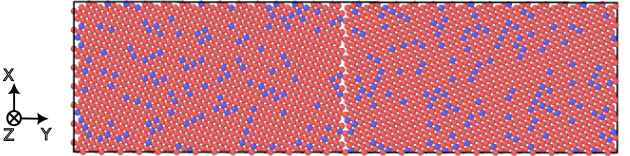
\includegraphics[width=0.70\textwidth]{configuration.png}
%DIFDELCMD < %%%
\DIFdelendFL \DIFaddbeginFL 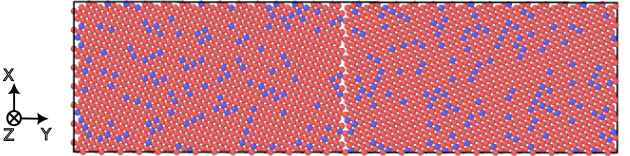
\includegraphics[height=3cm]{configuration.png}
\DIFaddendFL \caption{$\gamma$U-10Mo \{120\} symmetric tilt grain boundary at the initial configuration. Grain boundaries are in the middle and \DIFdelbeginFL \DIFdelFL{on }\DIFdelendFL \DIFaddbeginFL \DIFaddFL{along }\DIFaddendFL the edges of the supercell. Red atoms are uranium and blue atoms are molybdenum.}
\label{fig:gb}
\end{figure}

The dimensions of the supercells are at least $50 \text{ \r{A}} \times 200 \text{ \r{A}} \times 50 \text{ \r{A}}$, with the dimension perpendicular to the GB being the longest. These \DIFdelbegin \DIFdel{systems }\DIFdelend \DIFaddbegin \DIFadd{dimensions }\DIFaddend are verified to be large enough to obtain a stable system, from which converged energies can be extracted \cite{beeler2018}. A single simulation consists of 35000 to 50000 atoms depending on the type and misorientation angle of the GB. A temperature range starting from 600 K to 1200 K has been probed with an increment of 100 K. Three different compositions are investigated for symmetric tilt GB systems: $\gamma$U-7Mo \DIFaddbegin \DIFadd{(16 at.\% Mo)}\DIFaddend , $\gamma$U-10Mo \DIFaddbegin \DIFadd{(22 at.\% Mo)}\DIFaddend , and $\gamma$U-12Mo (\DIFdelbegin \DIFdel{in weight percent}\DIFdelend \DIFaddbegin \DIFadd{25 at.\% Mo}\DIFaddend ). For asymmetric tilt and twist GBs, only $\gamma$U-10Mo has been considered.
\DIFdelbegin \DIFdel{For any single GB at a given temperature, five simulations are performed }\DIFdelend \DIFaddbegin 

\DIFadd{An initial validation study is performed to ensure the correct construction of the GBs, measured against the reproducibility of GB energies in the literature. The GB energy is computed using the following equation.
}\begin{equation}
	E_{gb} = \bigg( \frac{E - E_0}{A} \bigg) N
\end{equation}
\DIFadd{where $E$ is the potential energy per atom of the system with GBs, $E_0$ is the potential energy per atom of the $\gamma$U-Mo system without GBs, $A$ is the area of the GBs, and $N$ is the number of atoms in the system with GBs. To obtain $E$, 25 simulations }\DIFaddend with different random number seeds \DIFaddbegin \DIFadd{are performed for each GB system}\DIFaddend . This allows for the evaluation of the statistical significance of the results since the seeds determine the initial distribution of Mo atoms and the velocities of both the U and Mo atoms in the supercell. \DIFaddbegin \DIFadd{Similarly, 25 simulations of $\gamma$U-Mo systems without a GB are conducted with different random number seeds to get an average reference energy $E_0$. The systems are relaxed over 100 ps in an NPT ensemble using a Nos\'e-Hoover thermostat at 1200 K, with energies averaged over the final 50 ps.
}\DIFaddend 

\DIFdelbegin \DIFdel{An initial validation study was performed to ensure the correct construction of the GBs, measured against the reproducibility of GB energies in the literature.
}\DIFdelend After validating the structures of GB systems, simulations are performed to extract the \DIFdelbegin \DIFdel{diffusion coefficients in the GBs}\DIFdelend \DIFaddbegin \DIFadd{GB diffusion coefficients}\DIFaddend . To that end, the supercells are first relaxed in an NPT ensemble using a \DIFdelbegin \DIFdel{Nose-Hoover }\DIFdelend \DIFaddbegin \DIFadd{Nos\'e-Hoover }\DIFaddend thermostat and barostat with a damping parameter of 0.1 ps. 100,000 \DIFdelbegin \DIFdel{steps are performed }\DIFdelend \DIFaddbegin \DIFadd{timesteps are run }\DIFaddend with a timestep \DIFaddbegin \DIFadd{size }\DIFaddend of 1 fs, making the NPT relaxation 100 ps in length. Afterward, the simulation box lengths are fixed at the equilibrated supercell lengths obtained during the NPT relaxation\DIFaddbegin \DIFadd{, }\DIFaddend and the systems are further equilibrated for 100 ps in an NVT ensemble. The NVT ensemble also uses a \DIFdelbegin \DIFdel{Nose-Hoover }\DIFdelend \DIFaddbegin \DIFadd{Nos\'e-Hoover }\DIFaddend thermostat with a 0.1 ps damping parameter. The production \DIFdelbegin \DIFdel{simulations }\DIFdelend \DIFaddbegin \DIFadd{runs }\DIFaddend are then executed for 5,000,000 \DIFdelbegin \DIFdel{steps }\DIFdelend \DIFaddbegin \DIFadd{timesteps }\DIFaddend with a timestep \DIFaddbegin \DIFadd{size }\DIFaddend of 2 fs, yielding a 10 ns \DIFdelbegin \DIFdel{trajectory for the determination of }\DIFdelend \DIFaddbegin \DIFadd{simulation for determining the }\DIFaddend diffusion coefficients. \DIFaddbegin \DIFadd{For a single GB structure, 5 simulations are performed with different random number seeds at a given temperature.
}\DIFaddend 

To examine the diffusion of Xe in $\gamma$U-Mo GBs, the $\gamma$U-10Mo symmetric tilt GBs are generated as per the prior procedure, but with a single Xe substitutional defect inserted in both GBs (a total of two Xe atoms in the system). For Xe simulations, the 100 ps NPT-ensemble relaxation and a subsequent 50 ps NVT-ensemble relaxation are first performed \DIFdelbegin \DIFdel{, }\DIFdelend \DIFaddbegin \DIFadd{and }\DIFaddend then Xe substitutions are made. After Xe insertion, the system is again relaxed in an NVT ensemble for 50 ps. A timestep \DIFaddbegin \DIFadd{size }\DIFaddend of 1 fs is used throughout the relaxation period. Afterward, a 100 ns data collection period begins with a timestep \DIFaddbegin \DIFadd{size }\DIFaddend of 5 fs. Since there are only two Xe atoms per system\DIFdelbegin \DIFdel{and Xe diffusion is slower than either U or Mo diffusion \cite{park2023}}\DIFdelend , collecting data over a longer period \DIFdelbegin \DIFdel{of time }\DIFdelend is necessary for diffusion calculations. \DIFaddbegin \DIFadd{5 simulations with different random number seeds are conducted for each GB system with Xe. It is also verified through a few simulations that changing the timestep size from 2 fs to 5 fs has minimal impact on the Xe trajectory and the stability of the simulations.
}\DIFaddend 

\DIFaddbegin \DIFadd{The GB region of the supercell is determined using the atomic trajectory images generated with OVITO \cite{ovito}. Atomic trajectories show where the lattice point jumps occur. Since almost all such jumps occur in the vicinity of the GB plane, the GB region can be differentiated from the bulk by determining the lattice points associated with the jumps. Figure \ref{fig:def} depicts how the GB region is defined as a rectangular cuboid in a system with symmetric tilt \{190\} GBs. Please notice that the GB region also includes lattice points that do not participate in the diffusion process. Tracking only mobile GB atoms would overestimate the diffusion coefficients and would not be representative of the GB structure. Once the GB region of a system is defined, the number of U and Mo atoms in that region is also recorded using OVITO's expression selection tool. To verify the GB width evaluated this way, the potential energy of the system as a function of the $y$ coordinate is also computed by averaging the potential energy over thin layers parallel to the GB plane. The peak widths of the potential energy graphs corroborate the determination of GB width $\delta_{gb}$ using atomic trajectories. Several atomic trajectories and potential energy peaks are analyzed for each GB system using different portions of the simulation data to detect any GB migration since the migration of a GB would likely yield spurious results. Only in a few high-temperature simulations was GB migration observed. The simulations showing GB migration are not used in the calculation of the diffusion coefficients.
}

\begin{figure}[!ht]
\centering
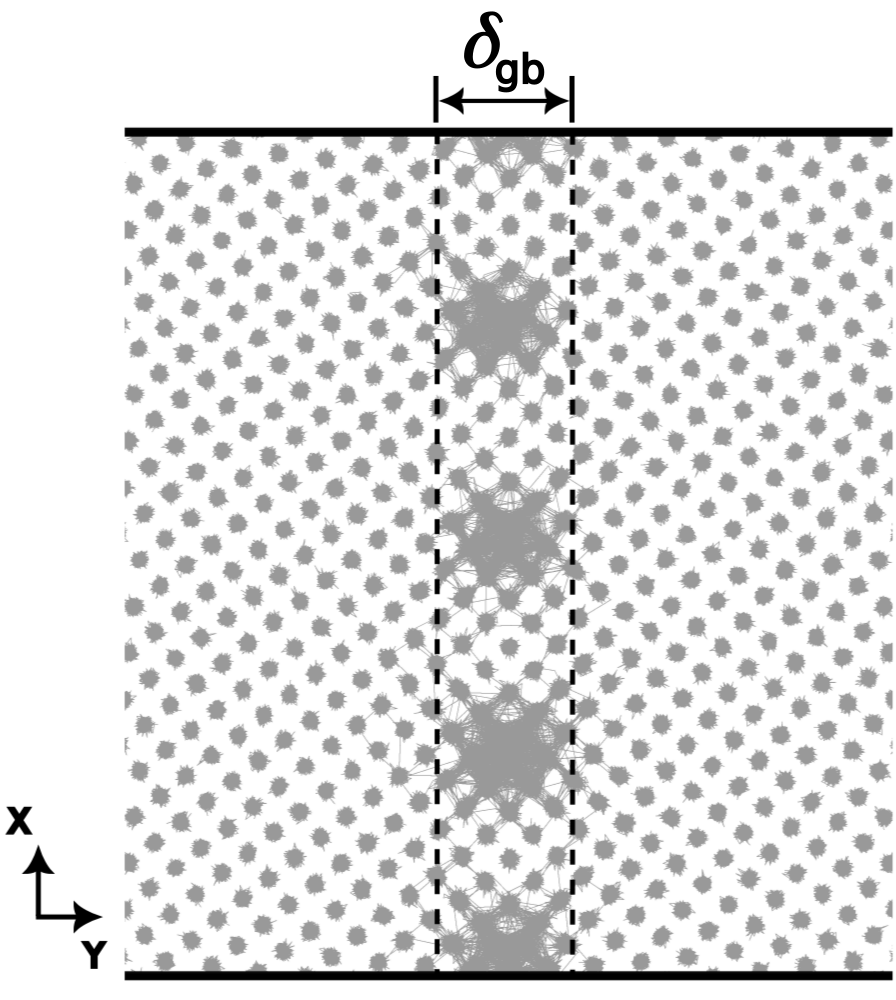
\includegraphics[height=6cm]{gb_def.png}
\caption{\DIFaddFL{Definition of the grain boundary region based on the trajectories of atoms in a $\gamma$U-10Mo supercell with symmetric tilt \{190\} grain boundary at 1100 K.}}
\label{fig:def}
\end{figure}

\DIFaddend To calculate the mean squared displacement (MSD) of the U, Mo, and Xe atoms in the \DIFdelbegin \DIFdel{GB}\DIFdelend \DIFaddbegin \DIFadd{systems}\DIFaddend , a buffer averaging scheme is deployed as described in \cite{rapaport2004}. In this scheme, multiple parallel MSD calculations are performed over subsets of the full simulations. For example, in the case of systems without Xe, the first buffer computes the MSD from 2 ns to 7 ns, and the second computes \DIFaddbegin \DIFadd{the }\DIFaddend MSD from 3 ns to 8 ns, and so on. MSD values from 4 such buffers are then averaged. While the average from only 4 buffers is enough to get a smooth MSD versus time curve of U and Mo atoms, MSD calculations of Xe need more buffers. Therefore, a total of 34 buffers, where each buffer calculates the MSD over 12.5 ns, are employed for the systems with Xe. The starting times of two successive buffers are separated by 2.5 ns in this case.
\DIFdelbegin \DIFdel{Once the buffer-averaged MSD values are available as a function of time, the Einstein relation can be }\DIFdelend \DIFaddbegin 

\DIFadd{The Einstein relation is }\DIFaddend used to compute the diffusion coefficients \DIFdelbegin \DIFdel{. The diffusion coefficients in the GB can then be calculated from Eq. \ref{eq:ein}:
}%DIFDELCMD < 

%DIFDELCMD < \begin{align}\label{eq:ein}
%DIFDELCMD < 	D_{GB} &= \frac{1}{2\xi} \frac{d \langle r^2 \rangle_{GB}}{dt}
%DIFDELCMD < \end{align}%%%
\DIFdelend \DIFaddbegin \DIFadd{from the buffer-averaged MSD values. The following equations are used to extract GB diffusion coefficients of U, Mo, and Xe perpendicular and parallel to the tilt axis,
}\begin{equation}
	D^i_{\perp} = \frac{N_{i, gb}}{N_i} \frac{\langle x^2 \rangle}{2 \Delta t}
\end{equation}\DIFaddend 
\DIFdelbegin \DIFdel{where $\xi$ is the dimensionality of the diffusion and $\langle r^2 \rangle_{GB}$ is the MSD of the }\DIFdelend \DIFaddbegin \begin{equation}
	D^i_{\parallel} = \frac{N_{i, gb}}{N_i} \frac{\langle z^2 \rangle}{2 \Delta t}
\end{equation}
\DIFadd{where $D^i_{\perp}$ is the GB diffusion coefficient of $i$ (=U, Mo, or Xe) perpendicular to the tilt axis, $D^i_{\parallel}$ is the GB diffusion coefficient of $i$ parallel to the tilt axis, $\Delta t$ is the corresponding simulation time of the directional MSDs $\langle x^2 \rangle$ or $\langle z^2 \rangle$ of the system, $N_i$ is the number of $i$ }\DIFaddend atoms in the \DIFdelbegin \DIFdel{GB}\DIFdelend \DIFaddbegin \DIFadd{system, and $N_{i, gb}$ is the number of $i$ atoms in the GB region. It is assumed that the atoms outside the GB region undergo negligible diffusion}\DIFaddend . \DIFdelbegin \DIFdel{The diffusion coefficients for all the aforementioned systems are calculated using this equation. Since the studied systems are two-dimensional GBs, the dimensionality is $\xi=2$. }\DIFdelend Generally, diffusion follows the Arrhenius equation as formulated \DIFdelbegin \DIFdel{in Eq. \ref{eq:arrD}:
}%DIFDELCMD < \begin{align}
%DIFDELCMD < 	\label{eq:arrD}
%DIFDELCMD < 	D &= D_0 \exp \bigg( -\frac{E_a}{k_B T} \bigg)
%DIFDELCMD < \end{align}%%%
\DIFdelend \DIFaddbegin \DIFadd{below,
}\begin{equation}
	D = D_0 \exp \bigg( -\frac{E_a}{k_B T} \bigg)
\end{equation}\DIFaddend 
where $D_0$ is the pre-exponential factor, $E_a$ is the activation energy, $T$ is the absolute temperature, and $k_B$ is the Boltzmann constant. Arrhenius fits \DIFdelbegin \DIFdel{are calculated for the diffusion coefficients of }\DIFdelend \DIFaddbegin \DIFadd{to the GB diffusion coefficients are calculated for }\DIFaddend all the simulated systems.


\section{Results}

\subsection{Grain boundary validation}

\DIFdelbegin \DIFdel{To check the validity of the constructed systems, GB energies for $\gamma$U-10Mo GBs are calculated to compare against literature values. The systems are relaxed over 100 ps in an NPT ensemble at 1200 K, with energies averaged over the final 50 ps, with 25 unique simulations performed for each GB system. The }\DIFdelend \DIFaddbegin \DIFadd{The }\DIFaddend symmetric tilt GB energies are shown in Figure \ref{fig:gbe}, with the error bars indicating $1\sigma$ confidence intervals. All symmetric tilt GB energies are within $2\sigma$ of the values reported \DIFdelbegin \DIFdel{in }\DIFdelend \DIFaddbegin \DIFadd{by }\DIFaddend Beeler et al. \cite{beeler2018}. Therefore, the computed GB energies in this work agree with the results from Beeler et al. It should be noted that the GB systems used by Beeler et al. have roughly 10 times fewer atoms. The average GB energy for the examined symmetric tilt GBs is 0.68 Jm$^{-2}$.

\begin{figure}[!ht]
\centering
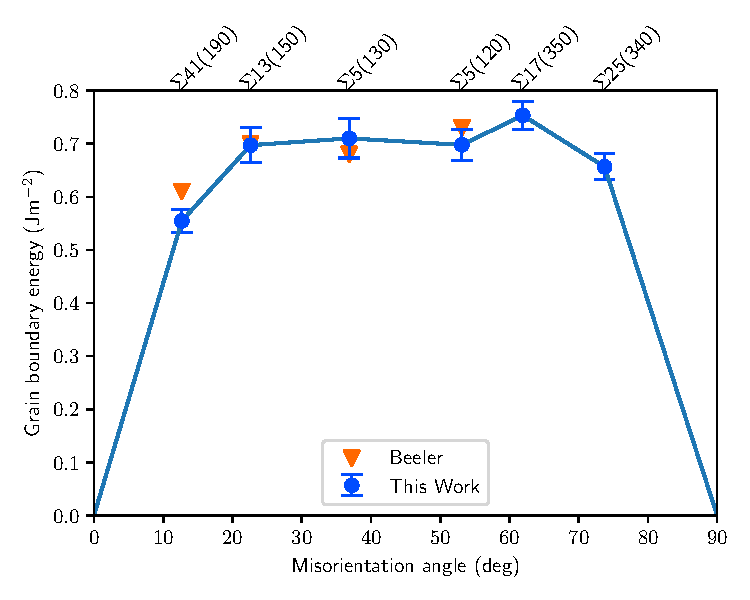
\includegraphics[width=0.70\textwidth]{gbe.pdf}
\caption{Grain boundary energies as a function of misorientation angle for $\gamma$U-10Mo symmetric tilt grain boundaries at 1200 K.}
\label{fig:gbe}
\end{figure}

\DIFaddbegin \begin{table}[!ht]
\centering
\caption{\DIFaddFL{Grain boundary energies of $\gamma$U-10Mo asymmetric tilt and twist grain boundaries at 1200 K.}}
\label{tab:gbe}
\begin{tabular}{cc}
\toprule
\DIFaddFL{GB plane }& \DIFaddFL{Energy (Jm$^{-2}$) }\\
\midrule
\DIFaddFL{asym  \{110\} }& \DIFaddFL{0.77 }\\
\DIFaddFL{asym  \{130\} }& \DIFaddFL{1.15 }\\
\DIFaddFL{asym  \{190\} }& \DIFaddFL{0.41 }\\
\DIFaddFL{asym  \{350\} }& \DIFaddFL{1.10 }\\
\DIFaddFL{twist \{110\} }& \DIFaddFL{0.84 }\\
\DIFaddFL{twist \{230\} }& \DIFaddFL{1.14 }\\
\bottomrule
\end{tabular}
\end{table}

\DIFaddend Novel asymmetric tilt and twist GBs are explored in this work which have not been studied previously. The energies of these GBs in $\gamma$U-10Mo are shown in Table \ref{tab:gbe}. The average GB energy is 0.90 Jm$^{-2}$ for the probed asymmetric tilt and twist GB systems. \DIFdelbegin \DIFdel{With the exception of the asymmetric }\DIFdelend \DIFaddbegin \DIFadd{Except for the asymmetric tilt }\DIFaddend \{190\} \DIFdelbegin \DIFdel{tilt }\DIFdelend GB, all the asymmetric tilt and twist GBs have higher GB energy than the symmetric tilt GBs. This means the asymmetric tilt and twist GBs are \DIFdelbegin \DIFdel{generally }\DIFdelend \DIFaddbegin \DIFadd{in general }\DIFaddend energetically less favorable to form than the symmetric tilt GBs.


\DIFdelbegin %DIFDELCMD < \begin{table}[!ht]
%DIFDELCMD < \centering
%DIFDELCMD < %%%
%DIFDELCMD < \caption{%
{%DIFAUXCMD
\DIFdelFL{Grain boundary energies of $\gamma$U-10Mo asymmetric tilt and twist grain boundaries at 1200 K.}}
%DIFAUXCMD
%DIFDELCMD < \label{tab:gbe}
%DIFDELCMD < \begin{tabular}{lc}
%DIFDELCMD < \toprule
%DIFDELCMD < %%%
\DIFdelFL{GB plane }%DIFDELCMD < & %%%
\DIFdelFL{Energy (Jm$^{-2}$) }%DIFDELCMD < \\
%DIFDELCMD < \midrule
%DIFDELCMD < %%%
\DIFdelFL{asym \{110\} }%DIFDELCMD < & %%%
\DIFdelFL{0.77 }%DIFDELCMD < \\
%DIFDELCMD < %%%
\DIFdelFL{asym \{130\} }%DIFDELCMD < & %%%
\DIFdelFL{1.15 }%DIFDELCMD < \\
%DIFDELCMD < %%%
\DIFdelFL{asym \{190\} }%DIFDELCMD < & %%%
\DIFdelFL{0.41 }%DIFDELCMD < \\
%DIFDELCMD < %%%
\DIFdelFL{asym \{350\} }%DIFDELCMD < & %%%
\DIFdelFL{1.10 }%DIFDELCMD < \\
%DIFDELCMD < %%%
\DIFdelFL{twist \{110\} }%DIFDELCMD < & %%%
\DIFdelFL{0.84 }%DIFDELCMD < \\
%DIFDELCMD < %%%
\DIFdelFL{twist \{230\} }%DIFDELCMD < & %%%
\DIFdelFL{1.14 }%DIFDELCMD < \\
%DIFDELCMD < \bottomrule
%DIFDELCMD < \end{tabular}
%DIFDELCMD < \end{table}
%DIFDELCMD < 

%DIFDELCMD < %%%
\DIFdelend \FloatBarrier
\subsection{Temperature-dependent \DIFdelbegin \DIFdel{GB }\DIFdelend \DIFaddbegin \DIFadd{grain boundary }\DIFaddend width}\label{sec:res1}

\DIFdelbegin \DIFdel{In order to correctly identify the GB diffusion, }\DIFdelend \DIFaddbegin \DIFadd{There are different kinds of GB widths defined in various ways. The diffusional width $\delta_D$ of a GB is defined using }\DIFaddend the number of \DIFdelbegin \DIFdel{GB }\DIFdelend \DIFaddbegin \DIFadd{mobile GB atoms so that the MSD of all }\DIFaddend atoms \DIFdelbegin \DIFdel{, often approximated using the GB width, needs to be determined. Figure \ref{fig:hist} shows the histogram of the squared displacements of all atoms . Atoms with a squared displacement of less than $3$ \r{A}$^2$ are assumed to be vibrating about their lattice positions, and not contributing to the net diffusion . In the systems with }\DIFdelend \DIFaddbegin \DIFadd{in the system can be used to compute the double product $D_{gb} \delta_D$ (also called the diffusion flux). The diffusional width is not the same as the structural width $\delta_{gb}$ of }\DIFaddend a GB, \DIFdelbegin \DIFdel{this comprises the majority of atoms in the system. The second peak of the histogram appears at $9$ \r{A}$^2$, which is close to the square of the average nearest neighbor distance in U-10Mo (around $3$ \r{A}). Other peaks are found also at squares of multiples of the nearest neighbor distance. OVITO is usedto visually inspect the atoms having more than $3$ \r{A}$^2$ squared displacement \cite{ovito}. Through the inspection of atomic trajectories, it is confirmed that these atoms constitute the GBs in the system. Thus, }\DIFdelend \DIFaddbegin \DIFadd{which can be defined using the total number of atoms residing within the GB region \cite{peterson1986, keblinski1999}. However, }\DIFaddend the \DIFdelbegin \DIFdel{sum of }\DIFdelend \DIFaddbegin \DIFadd{definition of the GB region may vary depending on the method used. Thus, the determination of the GB region is not straightforward. In literature, atom coordination, potential energy peak width, and other properties have been used for this purpose \cite{riet2021, koju2020}. Assuming a fixed value for $\delta_{gb}$ is also quite common and the assumptions fall between 5 \r{A} to 15 \r{A} \cite{suzuki2005, cooper2021, popov2022}. In this work, "GB width" means the structural width of a GB, and the definition of }\DIFaddend the \DIFdelbegin \DIFdel{squared displacement of atoms having more than $3$ \r{A}$^2$ squared displacement is equivalent to the total squared displacement of the GB atoms. GB MSD can then be determined from that displacement by averaging over the number of atoms that are participating in the diffusion process}\DIFdelend \DIFaddbegin \DIFadd{GB region is based on the lattice points that facilitate the diffusion of atoms}\DIFaddend .

\DIFdelbegin %DIFDELCMD < \begin{figure}[!ht]
%DIFDELCMD < \centering
%DIFDELCMD < 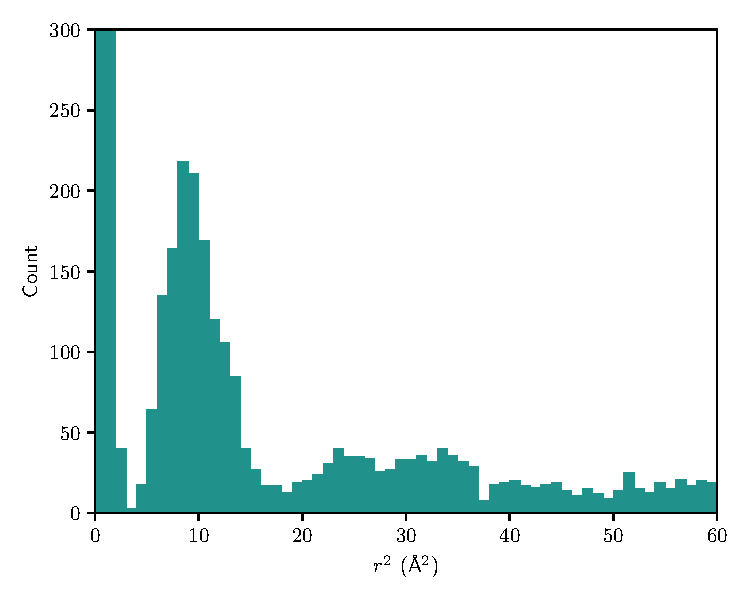
\includegraphics[width=0.60\textwidth]{histogram.pdf}
%DIFDELCMD < %%%
%DIFDELCMD < \caption{%
{%DIFAUXCMD
\DIFdelFL{Histogram of squared displacements of atoms in a $\gamma$U-10Mo simulation at 1200 K. The histogram bars on the domain x$\in$}%DIFDELCMD < [%%%
\DIFdelFL{0,2}%DIFDELCMD < ] %%%
\DIFdelFL{are curtailed to better illustrate the data.}}
%DIFAUXCMD
%DIFDELCMD < \label{fig:hist}
%DIFDELCMD < \end{figure}
%DIFDELCMD < 

%DIFDELCMD < %%%
\DIFdel{The number of diffusing atoms is plotted against inverse temperature for the symmetric tilt\{120\} GB in }\DIFdelend \DIFaddbegin \DIFadd{Figure \ref{fig:delta} displays the GB width $\delta_{gb}$ as a function of temperature for symmetric tilt, asymmetric tilt, and twist grain boundaries in $\gamma$}\DIFaddend U-10Mo\DIFdelbegin \DIFdel{in Figure \ref{fig:atomVsT}. The simulation box for this orientation has 36,864 total atoms}\DIFdelend . \DIFaddbegin \DIFadd{The widths of symmetric tilt GBs in $\gamma$U-7Mo and $\gamma$U-12Mo are similar to that in $\gamma$U-10Mo. }\DIFaddend It is observed that \DIFdelbegin \DIFdel{the number of diffusing GB atoms increases with increasing temperature. The percentage of atoms participating in diffusion rises from $0.7\%$ }\DIFdelend \DIFaddbegin \DIFadd{GB width has a positive correlation with temperature. In all cases, the GB width increases from about 6 \r{A} }\DIFaddend at 600 \DIFdelbegin \DIFdel{K to $12.7\%$ at 1200 K. This increase is almost exponential in nature. This correlates physically to an effective GB width that increases from 0.1 nm at 600 }\DIFdelend K to \DIFdelbegin \DIFdel{1.4 nm }\DIFdelend \DIFaddbegin \DIFadd{about 12 \r{A} }\DIFaddend at 1200 K \DIFdelbegin \DIFdel{. The effective GB width is calculated using the formula $w = \frac{DA}{TA} \frac{L_y}{2}$, where $DA$ and $TA$ are the number of diffusing atoms and the number of total atoms in the system, respectively, and $L_y$ is the length of the supercell in the direction perpendicular to the GBs. $L_y$ is divided by two due to the two GBs present in the supercell. The effective GB width defined here is similar to the notion of diffusional width as described in \cite{keblinski1999}. The }\DIFdelend \DIFaddbegin \DIFadd{almost linearly. The computed GB widths are close to the values found in the literature. The }\DIFaddend result here depicts that assuming a fixed GB width across temperatures, as \DIFdelbegin \DIFdel{it }\DIFdelend has been done for U$_3$Si$_2$ \cite{cooper2021}, would have been erroneous for the \DIFaddbegin \DIFadd{$\gamma$}\DIFaddend U-Mo system.

\begin{figure}[!ht]
\DIFaddbeginFL \begin{subfigure}{0.49\textwidth}
	\DIFaddendFL \centering
	\DIFdelbeginFL %DIFDELCMD < 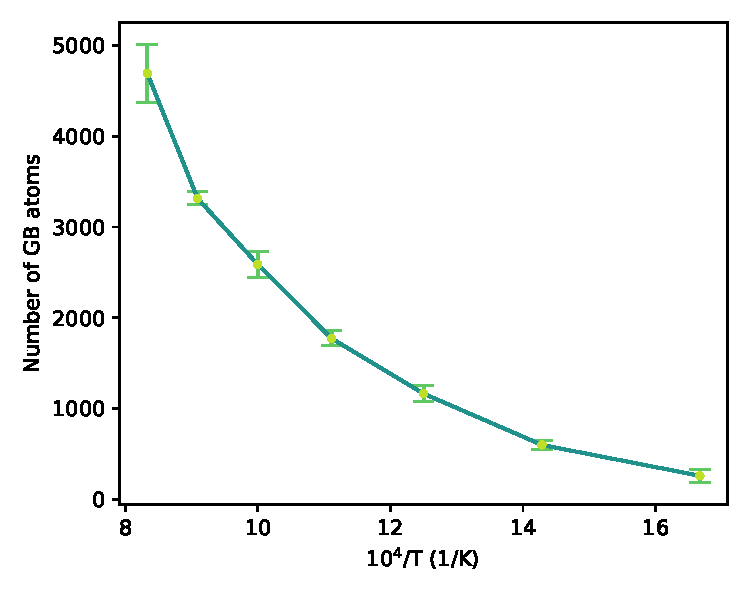
\includegraphics[width=0.60\textwidth]{atomsVsT.pdf}
%DIFDELCMD < %%%
\DIFdelendFL \caption{\DIFdelbeginFL \DIFdelFL{Number of grain boundary atoms as a function of temperature for symmetric tilt \{120\} in $\gamma$U-10Mo.}\DIFdelendFL }
	\DIFdelbeginFL %DIFDELCMD < \label{fig:atomVsT}
%DIFDELCMD < %%%
\DIFdelendFL \DIFaddbeginFL 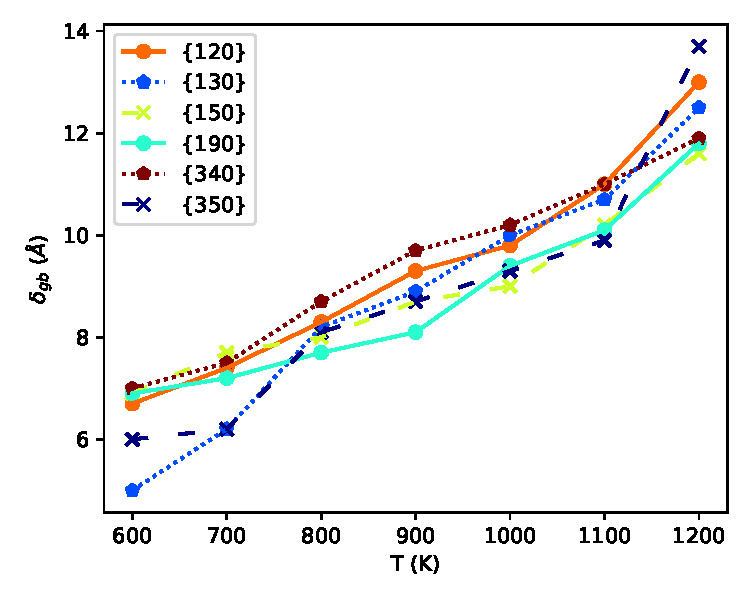
\includegraphics[width=\textwidth]{d_gb_sym.pdf}
\end{subfigure}
\begin{subfigure}{0.49\textwidth}
	\centering
	\caption{}
	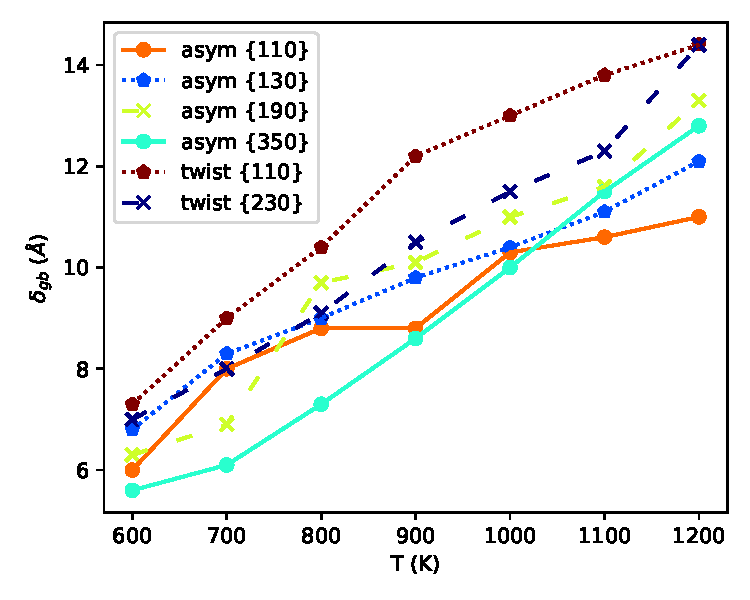
\includegraphics[width=\textwidth]{d_gb_asym_twist.pdf}
\end{subfigure}
\caption{\DIFaddFL{Grain boundary width of (a) symmetric tilt, and (b) asymmetric tilt and twist grain boundaries in $\gamma$U-10Mo as a function of temperature.}}
\label{fig:delta}
\DIFaddendFL \end{figure}

\FloatBarrier
\subsection{\DIFdelbegin \DIFdel{Total }\DIFdelend \DIFaddbegin \DIFadd{Grain boundary }\DIFaddend diffusion coefficients}

The \DIFdelbegin \DIFdel{total }\DIFdelend diffusion coefficients of \DIFaddbegin \DIFadd{U, Mo, and Xe (both perpendicular and parallel to the tilt axis) in }\DIFaddend various symmetric tilt GBs in $\gamma$U-10Mo are shown in Figure \ref{fig:u10mo}\DIFdelbegin \DIFdel{(a)}\DIFdelend . The diffusion behavior is generally Arrhenius, and the spread in diffusion coefficients due to tilt angles is \DIFdelbegin \DIFdel{within }\DIFdelend \DIFaddbegin \DIFadd{about }\DIFaddend one order of magnitude, regardless of the temperature. The order of magnitude of diffusion coefficients ranges from \DIFdelbegin \DIFdel{$10^{-11}$ }\DIFdelend \DIFaddbegin \DIFadd{$10^{-14}$ }\DIFaddend m$^2$s$^{-1}$ in the \DIFdelbegin \DIFdel{high-temperature region to $10^{-12}$ }\DIFdelend \DIFaddbegin \DIFadd{low-temperature region to $10^{-11}$ }\DIFaddend m$^2$s$^{-1}$ in the \DIFdelbegin \DIFdel{low-temperature }\DIFdelend \DIFaddbegin \DIFadd{high-temperature }\DIFaddend region. The standard deviation of diffusion coefficients at \DIFdelbegin \DIFdel{1200 K is around $10^{-12}$ }\DIFdelend \DIFaddbegin \DIFadd{600 K is of the order $10^{-14}$ }\DIFaddend m$^2$s$^{-1}$\DIFdelbegin \DIFdel{on average}\DIFdelend , while at \DIFdelbegin \DIFdel{600 }\DIFdelend \DIFaddbegin \DIFadd{1200 }\DIFaddend K it is \DIFdelbegin \DIFdel{around $10^{-13}$ }\DIFdelend \DIFaddbegin \DIFadd{of the order $10^{-12}$ }\DIFaddend m$^2$s$^{-1}$\DIFdelbegin \DIFdel{on average}\DIFdelend , with the standard deviation monotonically increasing with temperature. Error bars are excluded from the figure for readability. \DIFdelbegin \DIFdel{The }\DIFdelend \DIFaddbegin \DIFadd{For any symmetric tilt GB, the U GB diffusivities are higher than the Mo GB diffusivities. The Xe GB diffusivities are similar to the Mo GB diffusivities at low temperatures and to the U GB diffusivities at high temperatures. The }\DIFaddend pre-exponential factors and activation energies from the Arrhenius fits are listed in Table \ref{tab:u10moArr}. The \DIFdelbegin \DIFdel{table lists values }\DIFdelend \DIFaddbegin \DIFadd{activation energy is 0.4-0.7 eV }\DIFaddend for U GB diffusion, \DIFaddbegin \DIFadd{0.4-0.6 eV for }\DIFaddend Mo GB diffusion, and \DIFdelbegin \DIFdel{total GB diffusion. The activation energy for total diffusion is about 0.2-0.3 eV for the examined GBs }\DIFdelend \DIFaddbegin \DIFadd{0.5-0.8 eV for Xe GB diffusion }\DIFaddend in $\gamma$U-10Mo. This energy can be compared to the migration energies of point defect diffusion in $\gamma$U-10Mo. A recent study by Park et al. reports the migration energies of interstitial and vacancy diffusion of U in $\gamma$U-10Mo to be 0.40 eV and 0.73 eV, respectively \cite{park2023}. The \DIFaddbegin \DIFadd{magnitude of the }\DIFaddend activation energy of diffusion in the GB being \DIFdelbegin \DIFdel{lower than }\DIFdelend \DIFaddbegin \DIFadd{similar to }\DIFaddend the migration energies of \DIFaddbegin \DIFadd{the }\DIFaddend point defects indicates that the GB diffusion is \DIFdelbegin \DIFdel{not solely }\DIFdelend \DIFaddbegin \DIFadd{mostly }\DIFaddend mediated by the migration of point defects.
\DIFdelbegin \DIFdel{It also suggests that the GBs in $\gamma$U-Mo have highly disordered regions, where discernible point defects might be nonexistent.
}\DIFdelend 

\begin{figure}[!ht]
\DIFdelbeginFL %DIFDELCMD < \begin{subfigure}{\textwidth}
%DIFDELCMD < 	%%%
\DIFdelendFL \centering
\DIFaddbeginFL \begin{subfigure}{0.45\textwidth}
	\centering
	\DIFaddendFL \caption{}
	\DIFdelbeginFL %DIFDELCMD < 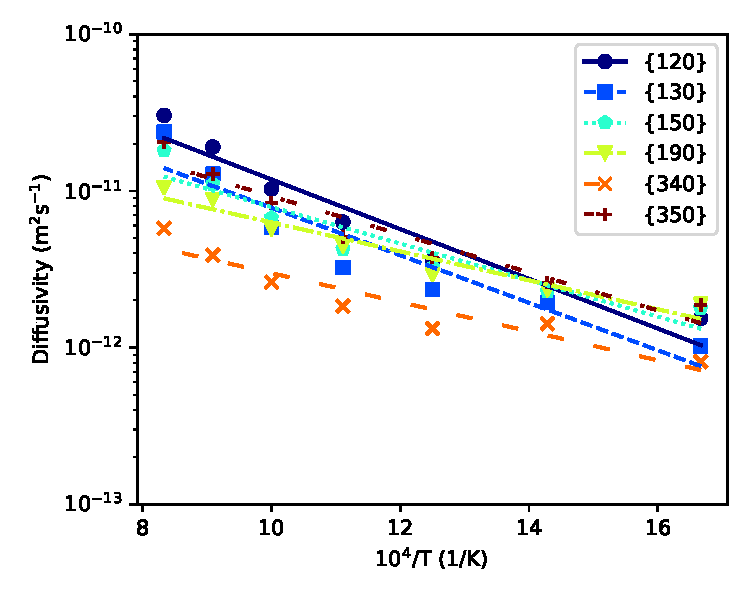
\includegraphics[width=0.65\textwidth]{u10mo_lin.pdf}
%DIFDELCMD < %%%
\DIFdelendFL \DIFaddbeginFL 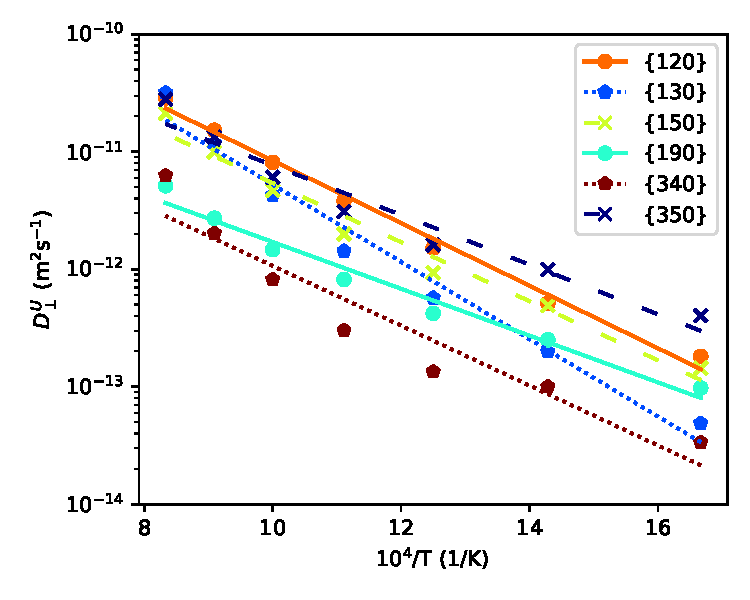
\includegraphics[height=5cm]{u10mo_U_Dx.pdf}
\DIFaddendFL \end{subfigure}
\DIFdelbeginFL %DIFDELCMD < 

%DIFDELCMD < \begin{subfigure}{\textwidth}
%DIFDELCMD < 	%%%
\DIFdelendFL \DIFaddbeginFL \begin{subfigure}{0.45\textwidth}
	\DIFaddendFL \centering
	\caption{}
	\DIFdelbeginFL %DIFDELCMD < 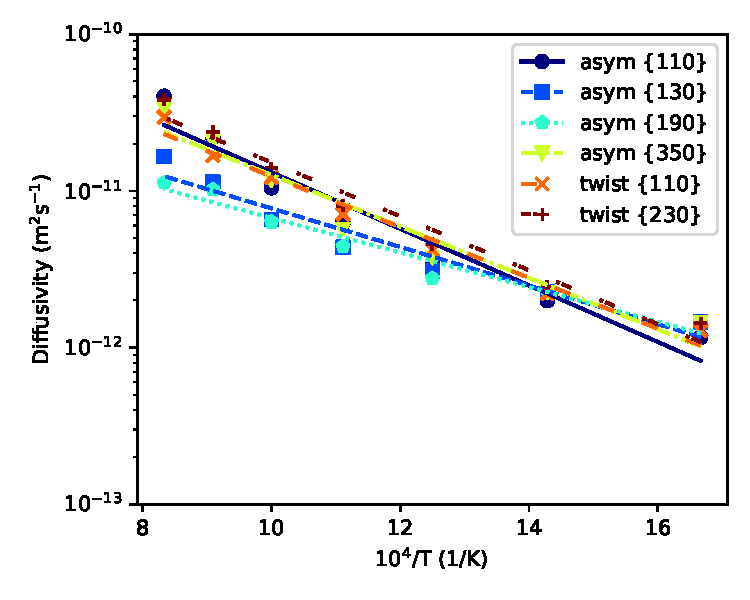
\includegraphics[width=0.65\textwidth]{asym_twist_lin.pdf}
%DIFDELCMD < %%%
\DIFdelendFL \DIFaddbeginFL 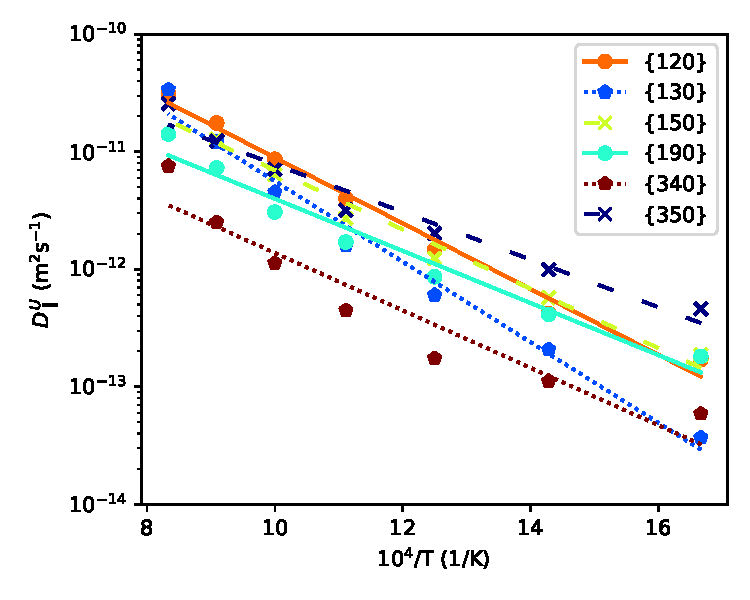
\includegraphics[height=5cm]{u10mo_U_Dz.pdf}
\DIFaddendFL \end{subfigure}
\DIFaddbeginFL \begin{subfigure}{0.45\textwidth}
	\centering
	\DIFaddendFL \caption{\DIFdelbeginFL \DIFdelFL{Total diffusivity in (a) symmetric tilt grain boundaries and (b) asymmetric tilt and twist grain boundaries for $\gamma$U-10Mo as a function of inverse temperature. Solid and dashed lines are Arrhenius fits to the data points.}\DIFdelendFL }
	\DIFaddbeginFL 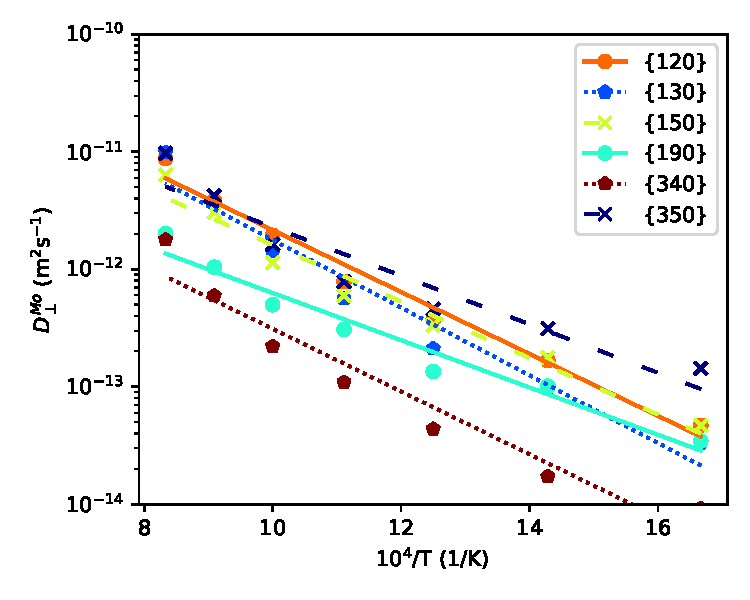
\includegraphics[height=5cm]{u10mo_Mo_Dx.pdf}
\end{subfigure}
\begin{subfigure}{0.45\textwidth}
	\centering
	\caption{}
	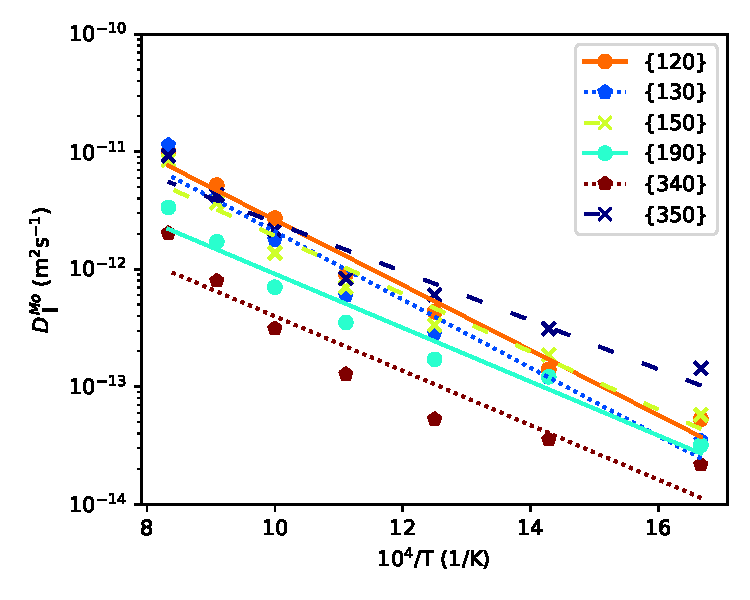
\includegraphics[height=5cm]{u10mo_Mo_Dz.pdf}
\end{subfigure}
\begin{subfigure}{0.45\textwidth}
	\centering
	\caption{}
	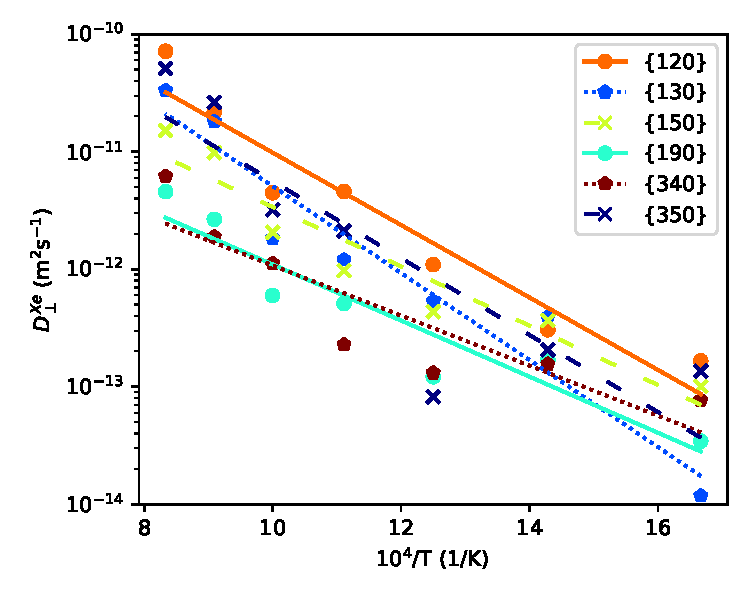
\includegraphics[height=5cm]{u10mo_Xe_Dx.pdf}
\end{subfigure}
\begin{subfigure}{0.45\textwidth}
	\centering
	\caption{}
	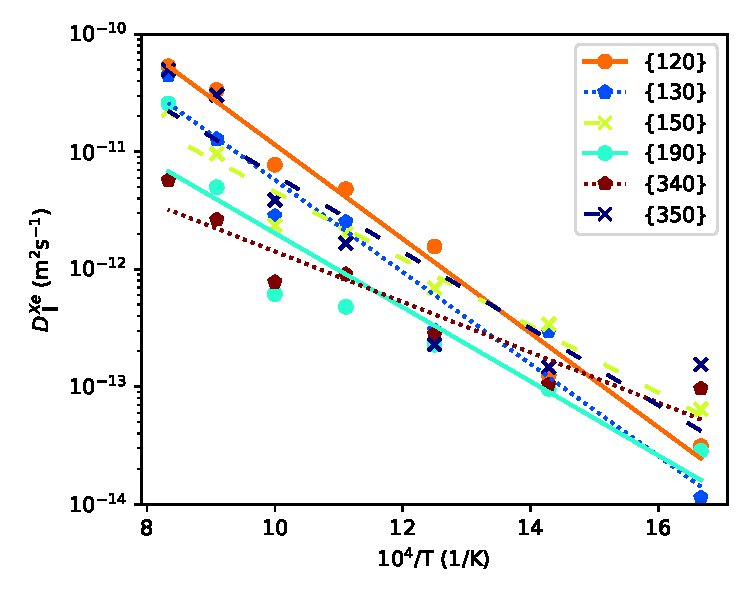
\includegraphics[height=5cm]{u10mo_Xe_Dz.pdf}
\end{subfigure}
\caption{\DIFaddFL{Diffusion coefficients of U (a) perpendicular and (b) parallel to the tilt axis, of Mo (c) perpendicular and (d) parallel to the tilt axis, and of Xe (e) perpendicular and (f) parallel to the tilt axis in symmetric tilt grain boundaries in $\gamma$U-10Mo as a function of inverse temperature. The lines are Arrhenius fits to the data points.}}
\DIFaddendFL \label{fig:u10mo}
\end{figure}

\begin{table}[!ht]
\centering
\caption{Prefactors and activation energies for the Arrhenius equation fits \DIFdelbeginFL \DIFdelFL{for }\DIFdelendFL \DIFaddbeginFL \DIFaddFL{to the diffusion coefficients of }\DIFaddendFL various symmetric tilt grain boundaries in $\gamma$U-10Mo. \DIFaddbeginFL \DIFaddFL{$D_0$ is in m$^2$s$^{-1}$ and $E_a$ is in eV.}\DIFaddendFL }
\label{tab:u10moArr}
\DIFdelbeginFL %DIFDELCMD < \begin{tabular}{lllllll}
%DIFDELCMD < %%%
\DIFdelendFL \DIFaddbeginFL \begin{tabular}{ccllllll}
\DIFaddendFL \toprule
GB plane & \DIFdelbeginFL \DIFdelFL{$D_{0,gb}^U$      }\DIFdelendFL \DIFaddbeginFL \DIFaddFL{Dir.
	}\DIFaddendFL & \DIFdelbeginFL \DIFdelFL{$E_{a,gb}^U$
	 }\DIFdelendFL \DIFaddbeginFL \DIFaddFL{$D_{0}^U$     }\DIFaddendFL & \DIFdelbeginFL \DIFdelFL{$D_{0,gb}^{Mo}$   }\DIFdelendFL \DIFaddbeginFL \DIFaddFL{$E_{a}^U$
	}\DIFaddendFL & \DIFdelbeginFL \DIFdelFL{$E_{a,gb}^{Mo}$
	 }\DIFdelendFL \DIFaddbeginFL \DIFaddFL{$D_{0}^{Mo}$  }\DIFaddendFL & \DIFdelbeginFL \DIFdelFL{$D_{0,gb}^{Tot}$  }\DIFdelendFL \DIFaddbeginFL \DIFaddFL{$E_{a}^{Mo}$
	}\DIFaddendFL & \DIFdelbeginFL \DIFdelFL{$E_{a,gb}^{Tot}$ }\DIFdelendFL \DIFaddbeginFL \DIFaddFL{$D_{0}^{Xe}$  }& \DIFaddFL{$E_{a}^{Xe}$ }\DIFaddendFL \\
\midrule
\DIFdelbeginFL \DIFdelFL{\{120\} }\DIFdelendFL \DIFaddbeginFL \multirow{2}{*}{ \{120\} }
		\DIFaddendFL & \DIFdelbeginFL \DIFdelFL{5.39 }\DIFdelendFL \DIFaddbeginFL \DIFaddFL{$\perp$
		}& \DIFaddFL{3.87 $\times 10^{-09}$ }& \DIFaddFL{0.528
        }& \DIFaddFL{9.32 }\DIFaddendFL $\times 10^{-10}$ & \DIFdelbeginFL \DIFdelFL{0.322
        }\DIFdelendFL \DIFaddbeginFL \DIFaddFL{0.523
        }\DIFaddendFL & \DIFaddbeginFL \DIFaddFL{1.19 $\times 10^{-08}$ }& \DIFaddFL{0.612  }\\
        & \DIFaddFL{$\parallel$
		}& \DIFaddFL{5.57 $\times 10^{-09}$ }& \DIFaddFL{0.555
        }& \DIFaddFL{1.54 $\times 10^{-09}$ }& \DIFaddFL{0.549
		}& \DIFaddFL{1.17 $\times 10^{-07}$ }& \DIFaddFL{0.795  }\vspace{0.2cm } \\
\multirow{2}{*}{ \{130\} }
		& \DIFaddFL{$\perp$
		}& \DIFaddFL{1.02 $\times 10^{-08}$ }& \DIFaddFL{0.653
        }& \DIFaddendFL 1.35 \DIFaddbeginFL \DIFaddFL{$\times 10^{-09}$ }& \DIFaddFL{0.572
        }& \DIFaddFL{2.56 $\times 10^{-08}$ }& \DIFaddFL{0.734  }\\
        & \DIFaddFL{$\parallel$
		}& \DIFaddFL{1.50 $\times 10^{-08}$ }& \DIFaddFL{0.680
        }& \DIFaddFL{1.65 $\times 10^{-09}$ }& \DIFaddFL{0.575
        }& \DIFaddFL{4.73 $\times 10^{-08}$ }& \DIFaddFL{0.777  }\vspace{0.2cm } \\
\multirow{2}{*}{ \{150\} }
		& \DIFaddFL{$\perp$
		}& \DIFaddFL{1.77 $\times 10^{-09}$ }& \DIFaddFL{0.499
        }& \DIFaddFL{4.09 }\DIFaddendFL $\times 10^{-10}$ & \DIFdelbeginFL \DIFdelFL{0.271
        }\DIFdelendFL \DIFaddbeginFL \DIFaddFL{0.477
        }\DIFaddendFL & \DIFdelbeginFL \DIFdelFL{4.56 }\DIFdelendFL \DIFaddbeginFL \DIFaddFL{1.13 $\times 10^{-09}$ }& \DIFaddFL{0.501  }\\
        & \DIFaddFL{$\parallel$
		}& \DIFaddFL{2.33 $\times 10^{-09}$ }& \DIFaddFL{0.501
        }& \DIFaddFL{5.60 }\DIFaddendFL $\times 10^{-10}$ & \DIFdelbeginFL \DIFdelFL{0.315  }\DIFdelendFL \DIFaddbeginFL \DIFaddFL{0.489
        }& \DIFaddFL{3.19 $\times 10^{-09}$ }& \DIFaddFL{0.565  }\vspace{0.2cm } \DIFaddendFL \\
\DIFdelbeginFL \DIFdelFL{\{130\} }\DIFdelendFL \DIFaddbeginFL \multirow{2}{*}{ \{190\} }
		\DIFaddendFL & \DIFdelbeginFL \DIFdelFL{2.95 }\DIFdelendFL \DIFaddbeginFL \DIFaddFL{$\perp$
		}& \DIFaddFL{1.67 }\DIFaddendFL $\times 10^{-10}$ & \DIFdelbeginFL \DIFdelFL{0.308
        }\DIFdelendFL \DIFaddbeginFL \DIFaddFL{0.395
        }\DIFaddendFL & \DIFdelbeginFL \DIFdelFL{8.06 }\DIFdelendFL \DIFaddbeginFL \DIFaddFL{6.44 }\DIFaddendFL $\times 10^{-11}$ & \DIFdelbeginFL \DIFdelFL{0.242
        }\DIFdelendFL \DIFaddbeginFL \DIFaddFL{0.399
        }\DIFaddendFL & \DIFdelbeginFL \DIFdelFL{2.56 }\DIFdelendFL \DIFaddbeginFL \DIFaddFL{2.67 }\DIFaddendFL $\times 10^{-10}$ & \DIFdelbeginFL \DIFdelFL{0.301  }\DIFdelendFL \DIFaddbeginFL \DIFaddFL{0.474  }\DIFaddendFL \\
        \DIFdelbeginFL \DIFdelFL{\{150\} }\DIFdelendFL & \DIFdelbeginFL \DIFdelFL{1.38 }\DIFdelendFL \DIFaddbeginFL \DIFaddFL{$\parallel$
		}& \DIFaddFL{6.55 }\DIFaddendFL $\times 10^{-10}$ & \DIFdelbeginFL \DIFdelFL{0.239
        }\DIFdelendFL \DIFaddbeginFL \DIFaddFL{0.440
        }\DIFaddendFL & \DIFdelbeginFL \DIFdelFL{2.92 $\times 10^{-11}$ }\DIFdelendFL \DIFaddbeginFL \DIFaddFL{1.79 $\times 10^{-10}$ }\DIFaddendFL & \DIFdelbeginFL \DIFdelFL{0.173
        }\DIFdelendFL \DIFaddbeginFL \DIFaddFL{0.455
        }\DIFaddendFL & \DIFdelbeginFL \DIFdelFL{1.15 $\times 10^{-10}$ }\DIFdelendFL \DIFaddbeginFL \DIFaddFL{2.89 $\times 10^{-09}$ }\DIFaddendFL & \DIFdelbeginFL \DIFdelFL{0.231  }\DIFdelendFL \DIFaddbeginFL \DIFaddFL{0.626  }\vspace{0.2cm } \DIFaddendFL \\
\DIFdelbeginFL \DIFdelFL{\{190\} }\DIFdelendFL \DIFaddbeginFL \multirow{2}{*}{ \{340\} }
		\DIFaddendFL & \DIFdelbeginFL \DIFdelFL{5.94 $\times 10^{-11}$ }\DIFdelendFL \DIFaddbeginFL \DIFaddFL{$\perp$
		}\DIFaddendFL & \DIFdelbeginFL \DIFdelFL{0.187
        }\DIFdelendFL \DIFaddbeginFL \DIFaddFL{3.76 $\times 10^{-10}$ }\DIFaddendFL & \DIFdelbeginFL \DIFdelFL{2.13 $\times 10^{-11}$ }\DIFdelendFL \DIFaddbeginFL \DIFaddFL{0.505
        }\DIFaddendFL & \DIFdelbeginFL \DIFdelFL{0.161
        }\DIFdelendFL \DIFaddbeginFL \DIFaddFL{1.46 $\times 10^{-10}$ }\DIFaddendFL & \DIFdelbeginFL \DIFdelFL{5.27 $\times 10^{-11}$ }\DIFdelendFL \DIFaddbeginFL \DIFaddFL{0.530
        }\DIFaddendFL & \DIFdelbeginFL \DIFdelFL{0.183  }\DIFdelendFL \DIFaddbeginFL \DIFaddFL{1.46 $\times 10^{-10}$ }& \DIFaddFL{0.423  }\DIFaddendFL \\
        \DIFdelbeginFL \DIFdelFL{\{340\} }\DIFdelendFL & \DIFdelbeginFL \DIFdelFL{2.72 $\times 10^{-11}$ }\DIFdelendFL \DIFaddbeginFL \DIFaddFL{$\parallel$
		}\DIFaddendFL & \DIFdelbeginFL \DIFdelFL{0.186
        }\DIFdelendFL \DIFaddbeginFL \DIFaddFL{3.82 $\times 10^{-10}$ }\DIFaddendFL & \DIFdelbeginFL \DIFdelFL{1.39 }\DIFdelendFL \DIFaddbeginFL \DIFaddFL{0.485
        }& \DIFaddFL{8.27 }\DIFaddendFL $\times 10^{-11}$ & \DIFdelbeginFL \DIFdelFL{0.176
        }\DIFdelendFL \DIFaddbeginFL \DIFaddFL{0.460
        }\DIFaddendFL & \DIFdelbeginFL \DIFdelFL{2.53 $\times 10^{-11}$ }\DIFdelendFL \DIFaddbeginFL \DIFaddFL{1.97 $\times 10^{-10}$ }\DIFaddendFL & \DIFdelbeginFL \DIFdelFL{0.184  }\DIFdelendFL \DIFaddbeginFL \DIFaddFL{0.425  }\vspace{0.2cm } \DIFaddendFL \\
\DIFdelbeginFL \DIFdelFL{\{350\} }\DIFdelendFL \DIFaddbeginFL \multirow{2}{*}{ \{350\} }
		\DIFaddendFL & \DIFdelbeginFL \DIFdelFL{1.79 }\DIFdelendFL \DIFaddbeginFL \DIFaddFL{$\perp$
		}& \DIFaddFL{9.90 }\DIFaddendFL $\times 10^{-10}$ & \DIFdelbeginFL \DIFdelFL{0.248
        }\DIFdelendFL \DIFaddbeginFL \DIFaddFL{0.419
        }\DIFaddendFL & \DIFdelbeginFL \DIFdelFL{4.58 $\times 10^{-11}$ }\DIFdelendFL \DIFaddbeginFL \DIFaddFL{2.65 $\times 10^{-10}$ }\DIFaddendFL & \DIFdelbeginFL \DIFdelFL{0.197
        }\DIFdelendFL \DIFaddbeginFL \DIFaddFL{0.410
        }\DIFaddendFL & \DIFdelbeginFL \DIFdelFL{1.51 }\DIFdelendFL \DIFaddbeginFL \DIFaddFL{1.06 $\times 10^{-08}$ }& \DIFaddFL{0.650  }\\
        & \DIFaddFL{$\parallel$
		}& \DIFaddFL{8.28 }\DIFaddendFL $\times 10^{-10}$ & \DIFdelbeginFL \DIFdelFL{0.241  }\DIFdelendFL \DIFaddbeginFL \DIFaddFL{0.402
        }& \DIFaddFL{2.99 $\times 10^{-10}$ }& \DIFaddFL{0.413
        }& \DIFaddFL{1.17 $\times 10^{-08}$ }& \DIFaddFL{0.648  }\DIFaddendFL \\
\bottomrule
\end{tabular}
\end{table}

The \DIFdelbegin \DIFdel{diffusion coefficients for }\DIFdelend asymmetric tilt and twist \DIFdelbegin \DIFdel{GBs }\DIFdelend \DIFaddbegin \DIFadd{GB diffusion coefficients }\DIFaddend in $\gamma$U-10Mo are depicted in Figure \DIFdelbegin \DIFdel{\ref{fig:u10mo}(b). The variance in the diffusion coefficient with respect to orientation is very minor, and less than that for symmetric tilt GBs. The }\DIFdelend \DIFaddbegin \DIFadd{\ref{fig:asym}. The }\DIFaddend magnitude of the \DIFdelbegin \DIFdel{diffusivity }\DIFdelend \DIFaddbegin \DIFadd{diffusivities }\DIFaddend for non-symmetric tilt GBs \DIFdelbegin \DIFdel{is }\DIFdelend \DIFaddbegin \DIFadd{are }\DIFaddend in the same range as the symmetric tilt systems. Thus, the overall impact of the orientation of GBs on the diffusivity appears to be minimal. The data in Figure \DIFdelbegin \DIFdel{\ref{fig:u10mo}(b) still }\DIFdelend \DIFaddbegin \DIFadd{\ref{fig:asym} also }\DIFaddend show a general Arrhenius trend, and the prefactors and activation energies for these systems are tabulated in Table \ref{tab:asym} \DIFdelbegin \DIFdel{in }\DIFdelend \DIFaddbegin \DIFadd{of }\DIFaddend the appendix. The standard deviation in these systems is \DIFdelbegin \DIFdel{approximately $2.8 \times 10^{-12}$ }\DIFdelend \DIFaddbegin \DIFadd{of the order $10^{-14}$ }\DIFaddend m$^2$s$^{-1}$ at \DIFdelbegin \DIFdel{1200 }\DIFdelend \DIFaddbegin \DIFadd{600 }\DIFaddend K, and \DIFdelbegin \DIFdel{$2.8 \times 10^{-13}$ }\DIFdelend \DIFaddbegin \DIFadd{$ 10^{-12}$ }\DIFaddend m$^2$s$^{-1}$ at \DIFdelbegin \DIFdel{600 }\DIFdelend \DIFaddbegin \DIFadd{1200 }\DIFaddend K. The \DIFdelbegin \DIFdel{general errors for all systems are sufficiently small }\DIFdelend \DIFaddbegin \DIFadd{deviations for all the systems are small enough }\DIFaddend that the trends with respect to temperature are statistically significant.

\DIFdelbegin \DIFdel{The orientation-averaged values for }\DIFdelend \DIFaddbegin \begin{figure}[!ht]
\begin{subfigure}{0.49\textwidth}
	\centering
	\caption{}
	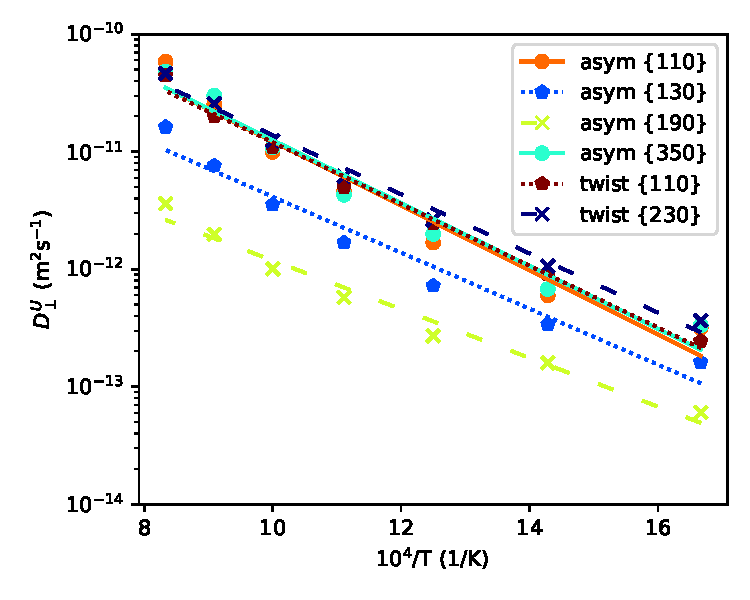
\includegraphics[width=\textwidth]{asym_twist_U_Dx.pdf}
\end{subfigure}
\begin{subfigure}{0.49\textwidth}
	\centering
	\caption{}
	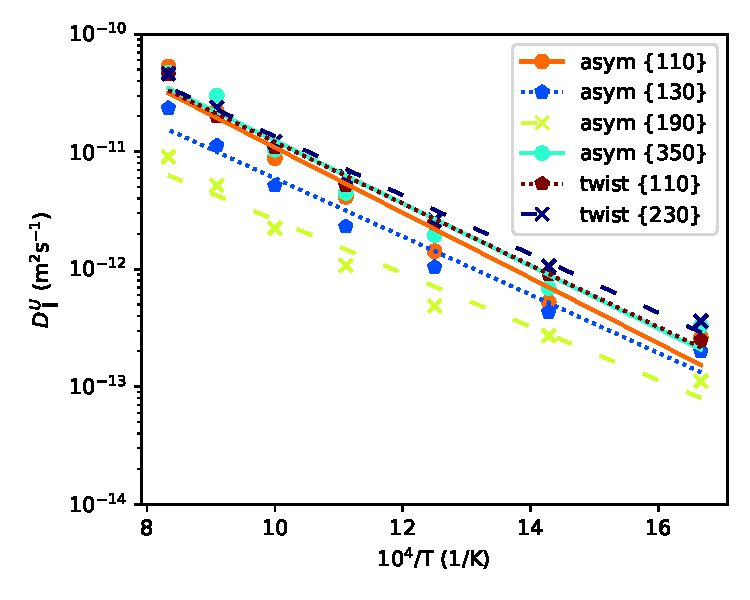
\includegraphics[width=\textwidth]{asym_twist_U_Dz.pdf}
\end{subfigure}

\begin{subfigure}{0.49\textwidth}
	\centering
	\caption{}
	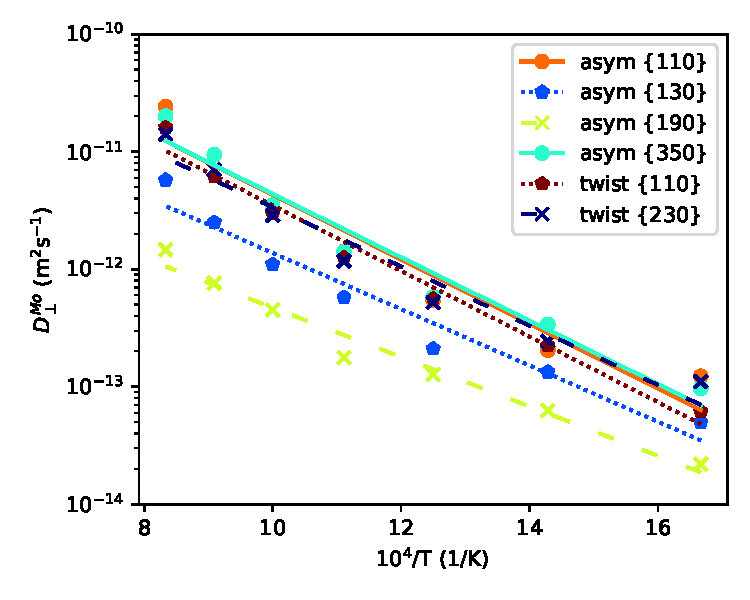
\includegraphics[width=\textwidth]{asym_twist_Mo_Dx.pdf}
\end{subfigure}
\begin{subfigure}{0.49\textwidth}
	\centering
	\caption{}
	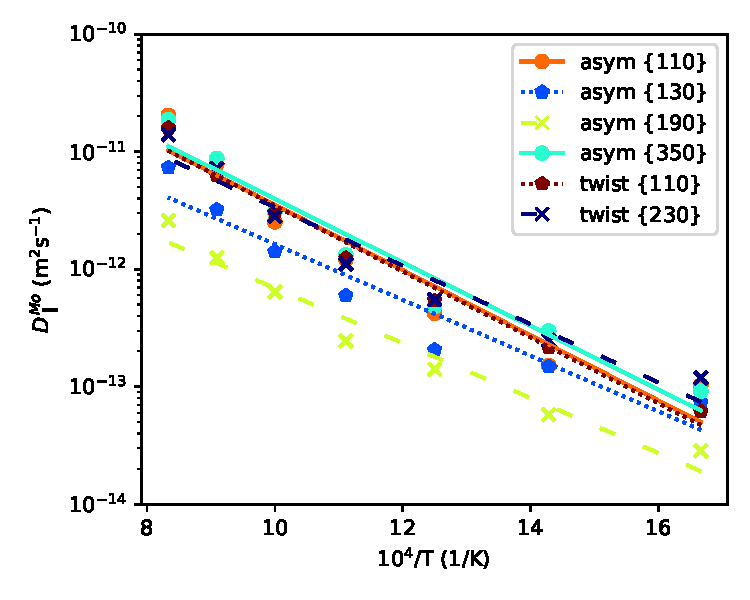
\includegraphics[width=\textwidth]{asym_twist_Mo_Dz.pdf}
\end{subfigure}
\caption{\DIFaddFL{Diffusion coefficients of U (a) perpendicular and (b) parallel to the tilt axis, and of Mo (c) perpendicular and (d) parallel to the tilt axis in asymmetric tilt and twist grain boundaries in $\gamma$U-10Mo as a function of inverse temperature. The lines are Arrhenius fits to the data points.}}
\label{fig:asym}
\end{figure}

\DIFadd{To compare the GB diffusion coefficients of }\DIFaddend $\gamma$U-7Mo, $\gamma$U-10Mo, and $\gamma$U-12Mo\DIFdelbegin \DIFdel{are shown in }\DIFdelend \DIFaddbegin \DIFadd{, the diffusion coefficients parallel to the tilt axis of all symmetric tilt GBs are averaged. We denote this orientation-averaged GB diffusion coefficient of species $i$ by $\overline{D}^i_{\parallel}$ for $i=$ U, Mo, or Xe. The rationale behind averaging $D^i_{\parallel}$ for comparison is that $D^i_{\parallel} > D^i_{\perp}$ for all kinds of GBs, even for the ones with high misorientation angles \cite{mishin2015}. The orientation-averaged U and Mo GB diffusion coefficients in different compositions are presented in }\DIFaddend Figure \ref{fig:comp}. While not shown, the range of diffusivities with respect to \DIFdelbegin \DIFdel{misorientation angles }\DIFdelend \DIFaddbegin \DIFadd{the misorientation angle }\DIFaddend in different compositions is also \DIFdelbegin \DIFdel{within }\DIFdelend \DIFaddbegin \DIFadd{about }\DIFaddend one order of magnitude, and thus only \DIFaddbegin \DIFadd{the }\DIFaddend orientation-averaged diffusivities are displayed. \DIFaddbegin \DIFadd{The general trend of the diffusivities as a function of temperature for the three examined compositions is identical. The standard deviations of the GB diffusivities in the $\gamma$U-7Mo and $\gamma$U-12Mo systems are also comparable to that of $\gamma$U-10Mo, which indicates the effect of composition on the diffusivities is not negligible. }\DIFaddend From the figure, it can be noticed that the \DIFaddbegin \DIFadd{GB }\DIFaddend diffusivity is negatively correlated with the Mo content of the fuel. This is \DIFdelbegin \DIFdel{somewhat }\DIFdelend expected as the U self-diffusivity is higher than that of Mo \cite{huang2013}, and \DIFaddbegin \DIFadd{thus }\DIFaddend increased Mo content suppresses \DIFdelbegin \DIFdel{self-diffusivity }\DIFdelend \DIFaddbegin \DIFadd{the GB diffusivities }\DIFaddend in $\gamma$U-Mo. \DIFdelbegin \DIFdel{The general trend as a function of the temperature of the diffusivity for the three examined compositions is identical. The standard deviations for the U-7Mo and U-12Mo systems are comparable to that of U-10Mo, which indicates that the trend observed with composition is statistically significant. }\DIFdelend Table \ref{tab:compArr} provides the Arrhenius \DIFdelbegin \DIFdel{parameters }\DIFdelend \DIFaddbegin \DIFadd{fits to the orientation-averaged GB diffusion coefficients }\DIFaddend for the different compositions. Also, the \DIFdelbegin \DIFdel{total GB diffusion coefficients for different tilts and temperatures }\DIFdelend \DIFaddbegin \DIFadd{Arrhenius fits to the diffusion coefficients of all the symmetric tilt GBs }\DIFaddend in $\gamma$U-7Mo and $\gamma$U-12Mo are listed in Tables \ref{tab:u7mo} and \ref{tab:u12mo} of the appendix for completeness.

\begin{figure}[!ht]
\DIFaddbeginFL \begin{subfigure}{0.49\textwidth}
	\DIFaddendFL \centering
	\DIFdelbeginFL %DIFDELCMD < 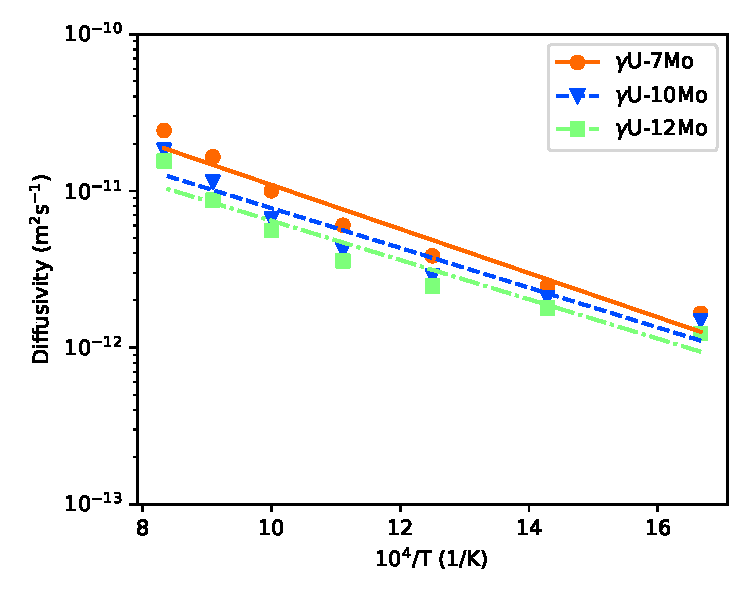
\includegraphics[width=0.70\textwidth]{composition_lin.pdf}
%DIFDELCMD < %%%
\DIFdelendFL \caption{\DIFdelbeginFL \DIFdelFL{Grain boundary orientation-averaged diffusion coefficients for $\gamma$U-7Mo, $\gamma$U-10Mo, and $\gamma$U-12Mo.}\DIFdelendFL }
	\DIFaddbeginFL 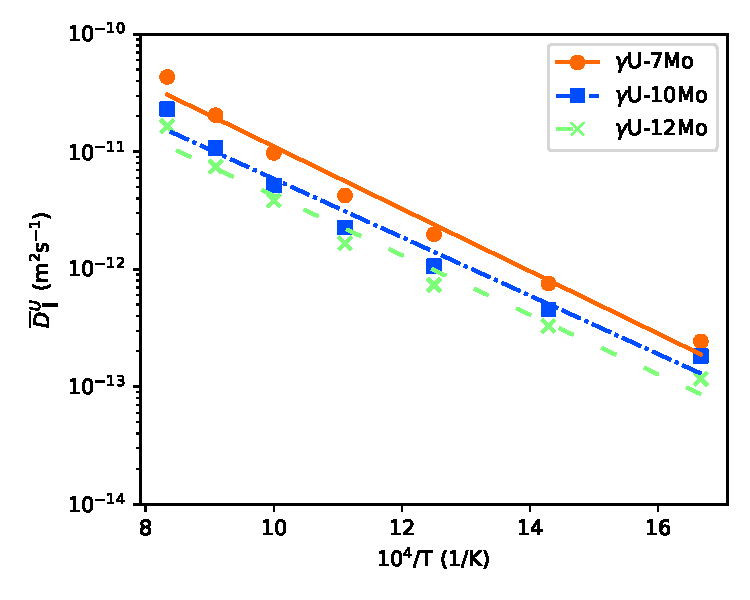
\includegraphics[width=\textwidth]{comp_U_Dz.pdf}
\end{subfigure}
\begin{subfigure}{0.49\textwidth}
	\centering
	\caption{}
	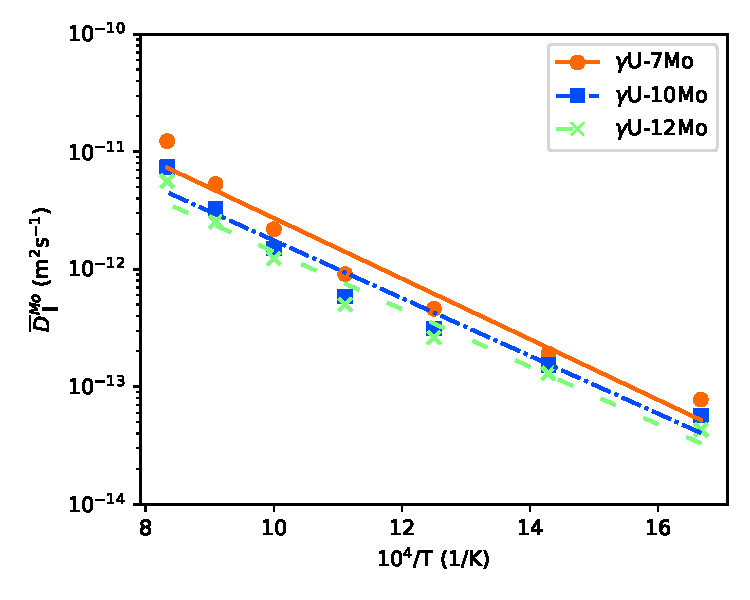
\includegraphics[width=\textwidth]{comp_Mo_Dz.pdf}
\end{subfigure}
\caption{\DIFaddFL{Orientation-averaged grain boundary diffusion coefficients of (a) U and (b) Mo parallel to the tilt axis for $\gamma$U-7Mo, $\gamma$U-10Mo, and $\gamma$U-12Mo.}}
\DIFaddendFL \label{fig:comp}
\end{figure}

\begin{table}[!ht]
\centering
\caption{Prefactors and activation energies for the Arrhenius equation fits \DIFdelbeginFL \DIFdelFL{for }\DIFdelendFL \DIFaddbeginFL \DIFaddFL{to the orientation-averaged }\DIFaddendFL grain boundary diffusion \DIFaddbeginFL \DIFaddFL{coefficients parallel to the tilt axis ($\overline{D}^{i}_{\parallel}$ for $i=$ U or Mo) }\DIFaddendFL in $\gamma$U-Mo alloys. \DIFaddbeginFL \DIFaddFL{$D_0$ is in m$^2$s$^{-1}$ and $E_a$ is in eV.}\DIFaddendFL }
\label{tab:compArr}
\DIFdelbeginFL %DIFDELCMD < \begin{tabular}{lllllll}
%DIFDELCMD < %%%
\DIFdelendFL \DIFaddbeginFL \begin{tabular}{cllll}
\DIFaddendFL \toprule
Composition
	& \DIFdelbeginFL \DIFdelFL{$D_{0,gb}^U$      }\DIFdelendFL \DIFaddbeginFL \DIFaddFL{$D_{0}^U$      }\DIFaddendFL & \DIFdelbeginFL \DIFdelFL{$E_{a,gb}^U$
	    }\DIFdelendFL \DIFaddbeginFL \DIFaddFL{$E_{a}^U$
	}\DIFaddendFL & \DIFdelbeginFL \DIFdelFL{$D_{0,gb}^{Mo}$   }\DIFdelendFL \DIFaddbeginFL \DIFaddFL{$D_{0}^{Mo}$   }\DIFaddendFL & \DIFdelbeginFL \DIFdelFL{$E_{a,gb}^{Mo}$
	    }%DIFDELCMD < & %%%
\DIFdelFL{$D_{0,gb}^{Tot}$  }%DIFDELCMD < & %%%
\DIFdelFL{$E_{a,gb}^{Tot}$ }\DIFdelendFL \DIFaddbeginFL \DIFaddFL{$E_{a}^{Mo}$ }\DIFaddendFL \\
\midrule
$\gamma$U-7Mo
	& \DIFdelbeginFL \DIFdelFL{3.12 $\times 10^{-10}$ }\DIFdelendFL \DIFaddbeginFL \DIFaddFL{4.98 $\times 10^{-09}$ }\DIFaddendFL & \DIFdelbeginFL \DIFdelFL{0.284 }\DIFdelendFL \DIFaddbeginFL \DIFaddFL{0.527
	}\DIFaddendFL & \DIFdelbeginFL \DIFdelFL{7.43 $\times 10^{-11}$
	       }\DIFdelendFL \DIFaddbeginFL \DIFaddFL{1.03 $\times 10^{-09}$ }\DIFaddendFL & \DIFdelbeginFL \DIFdelFL{0.231 }%DIFDELCMD < & %%%
\DIFdelFL{2.78 $\times 10^{-10}$ }%DIFDELCMD < & %%%
\DIFdelFL{0.279  }\DIFdelendFL \DIFaddbeginFL \DIFaddFL{0.511 }\DIFaddendFL \\
$\gamma$U-10Mo
	& \DIFdelbeginFL \DIFdelFL{1.68 $\times 10^{-10}$ }\DIFdelendFL \DIFaddbeginFL \DIFaddFL{1.80 $\times 10^{-09}$ }\DIFaddendFL & \DIFdelbeginFL \DIFdelFL{0.258 }\DIFdelendFL \DIFaddbeginFL \DIFaddFL{0.493
	}\DIFaddendFL & \DIFdelbeginFL \DIFdelFL{4.65 $\times 10^{-11}$
	       }%DIFDELCMD < & %%%
\DIFdelFL{0.210 }%DIFDELCMD < & %%%
\DIFdelFL{1.44 }\DIFdelendFL \DIFaddbeginFL \DIFaddFL{5.04 }\DIFaddendFL $\times 10^{-10}$ & \DIFdelbeginFL \DIFdelFL{0.252  }\DIFdelendFL \DIFaddbeginFL \DIFaddFL{0.488 }\DIFaddendFL \\
$\gamma$U-12Mo
	& \DIFdelbeginFL \DIFdelFL{1.38 $\times 10^{-10}$ }\DIFdelendFL \DIFaddbeginFL \DIFaddFL{1.44 $\times 10^{-09}$ }\DIFaddendFL & \DIFdelbeginFL \DIFdelFL{0.256 }\DIFdelendFL \DIFaddbeginFL \DIFaddFL{0.503
	}\DIFaddendFL & \DIFdelbeginFL \DIFdelFL{4.03 $\times 10^{-11}$
	       }%DIFDELCMD < & %%%
\DIFdelFL{0.206 }%DIFDELCMD < & %%%
\DIFdelFL{1.16 }\DIFdelendFL \DIFaddbeginFL \DIFaddFL{3.96 }\DIFaddendFL $\times 10^{-10}$ & \DIFdelbeginFL \DIFdelFL{0.249  }\DIFdelendFL \DIFaddbeginFL \DIFaddFL{0.486 }\DIFaddendFL \\
\bottomrule
\end{tabular}
\end{table}

\DIFdelbegin %DIFDELCMD < \FloatBarrier
%DIFDELCMD < %%%
\subsection{\DIFdel{Species diffusion coefficients}}
%DIFAUXCMD
\addtocounter{subsection}{-1}%DIFAUXCMD
%DIFDELCMD < 

%DIFDELCMD < %%%
\DIFdelend The orientation-averaged U, Mo, and Xe GB diffusion coefficients \DIFaddbegin \DIFadd{in $\gamma$U-10Mo }\DIFaddend are displayed in Figure \ref{fig:umoxe} \DIFdelbegin \DIFdel{. At high temperatures, all three species show GB diffusivity of the same order of magnitude}\DIFdelend \DIFaddbegin \DIFadd{along with U and Mo self-diffusivity, and intrinsic diffusivity of Xe in $\gamma$U-Mo from the literature}\DIFaddend . For all examined temperatures, \DIFaddbegin \DIFadd{the }\DIFaddend U GB diffusivity is \DIFdelbegin \DIFdel{roughly double }\DIFdelend \DIFaddbegin \DIFadd{higher than }\DIFaddend the GB diffusivity of Mo. The \DIFdelbegin \DIFdel{difference between the Xe GB diffusion coefficient and the U and Mo GB diffusion coefficients increases with decreasing temperature. Around }\DIFdelend \DIFaddbegin \DIFadd{Xe GB diffusivity is similar to the Mo GB diffusivity at }\DIFaddend 600 K \DIFdelbegin \DIFdel{, the Xe GB diffusion coefficient is approximately two orders of magnitude lower than that of }\DIFdelend \DIFaddbegin \DIFadd{and it steadily reaches the U GB diffusivity with increasing temperature. The }\DIFaddend U and Mo \DIFdelbegin \DIFdel{.
}%DIFDELCMD < 

%DIFDELCMD < \begin{figure}[!ht]
%DIFDELCMD < \centering
%DIFDELCMD < 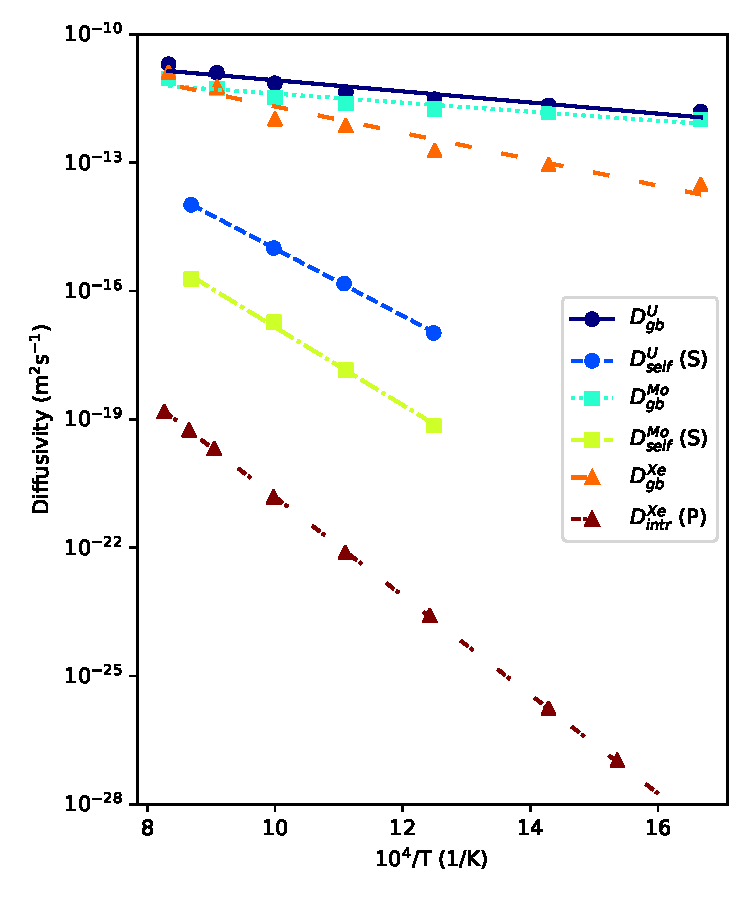
\includegraphics[width=0.80\textwidth]{comparison4.pdf}
%DIFDELCMD < %%%
%DIFDELCMD < \caption{%
{%DIFAUXCMD
\DIFdelFL{Orientation-averaged U, Mo, and Xe grain boundary diffusivities in $\gamma$U-10Mo with literature data. S represents the U and Mo self diffusivity in $\gamma$U-9Mo from Smirnova et al. \cite{smirnova2015}. P represents the intrinsic diffusivity of Xe in $\gamma$U-10Mo from Park et al. \cite{park2023}.}}
%DIFAUXCMD
%DIFDELCMD < \label{fig:umoxe}
%DIFDELCMD < \end{figure}
%DIFDELCMD < 

%DIFDELCMD < %%%
\DIFdel{Additional literature data on }\DIFdelend self-diffusivities in $\gamma$U-9Mo \DIFaddbegin \DIFadd{are extracted }\DIFaddend from Smirnova et al. \cite{smirnova2015}\DIFdelbegin \DIFdel{is included in Figure \ref{fig:umoxe} to provide perspective}\DIFdelend . These self-diffusivities were computed using the same ADP potential used for this work. Since the GB diffusivities of $\gamma$U-7Mo and $\gamma$U-10Mo are close, the difference in composition between the studies is not \DIFdelbegin \DIFdel{significant }\DIFdelend \DIFaddbegin \DIFadd{large }\DIFaddend enough to prevent \DIFdelbegin \DIFdel{a }\DIFdelend comparison. The GB diffusion coefficient of U is about three orders of magnitude higher than the self-diffusion coefficient \DIFdelbegin \DIFdel{at high temperatures}\DIFdelend \DIFaddbegin \DIFadd{around 1200 K}\DIFaddend . The difference between \DIFaddbegin \DIFadd{the }\DIFaddend GB diffusivity and \DIFaddbegin \DIFadd{the }\DIFaddend self-diffusivity grows larger with decreasing temperature. At around 800 K, the difference is about five orders of magnitude. For Mo, the GB diffusion coefficient is about four orders of magnitude higher than the self-diffusion coefficient \DIFdelbegin \DIFdel{at high temperatures}\DIFdelend \DIFaddbegin \DIFadd{around 1200 K}\DIFaddend , while the difference spans \DIFdelbegin \DIFdel{seven }\DIFdelend \DIFaddbegin \DIFadd{six }\DIFaddend orders of magnitude around 800 K. The intrinsic diffusion coefficient of Xe from Park et al. \cite{park2023} is included in the figure as well. This intrinsic diffusion coefficient was calculated using an EAM potential of U-Mo-Xe \cite{smirnova2013}. \DIFdelbegin \DIFdel{The difference between GB diffusion and intrinsic diffusion of Xe is more drastic than U and Mo. At high temperatures}\DIFdelend \DIFaddbegin \DIFadd{At 1200 K}\DIFaddend , the GB diffusion coefficient of Xe is about \DIFdelbegin \DIFdel{seven }\DIFdelend \DIFaddbegin \DIFadd{eight }\DIFaddend orders of magnitude higher than the intrinsic diffusion coefficient of Xe, while at 800 K, this enlarges to a difference of about \DIFdelbegin \DIFdel{ten }\DIFdelend \DIFaddbegin \DIFadd{eleven }\DIFaddend orders of magnitude. Table \ref{tab:enhance} summarizes the species-wise diffusion enhancements by GBs at four different temperatures.
\DIFdelbegin \DIFdel{It is apparent from the table that the diffusion enhancement is larger at lower temperatures. This means the overall diffusion in the material is dominated mostly by GB diffusion at lower temperatures, and thus GB diffusion is more important in the calculation of the effective diffusivity of the material.
The diffusion enhancement starts to wane at higher temperatures since the activation energy of GB diffusion is lower than that of bulk diffusion . This difference in activation energies is expected and is observable in Figure \ref{fig:umoxe}. Species-specific diffusion prefactors and activation energies are included in Tables \ref{tab:u10moArr}, \ref{tab:compArr}, \ref{tab:compArrHigh}, \ref{tab:compArrLow}, \ref{tab:u7mo}, \ref{tab:asym}, \ref{tab:u12mo}, and \ref{tab:xe}. 
}\DIFdelend 

\DIFaddbegin \begin{figure}[!ht]
\centering
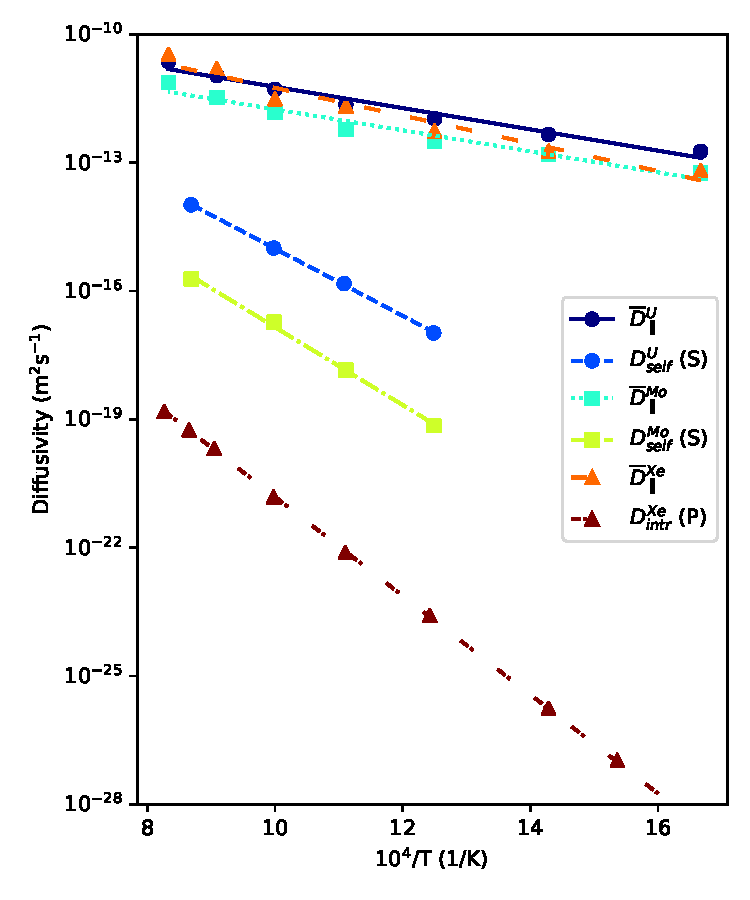
\includegraphics[width=0.70\textwidth]{newLitComp.pdf}
\caption{\DIFaddFL{Orientation-averaged U, Mo, and Xe grain boundary diffusivities parallel to the tilt axis in $\gamma$U-10Mo with literature data. S represents the U and Mo self-diffusivity in $\gamma$U-9Mo from Smirnova et al. \cite{smirnova2015}. P represents the intrinsic diffusivity of Xe in $\gamma$U-10Mo from Park et al. \cite{park2023}.}}
\label{fig:umoxe}
\end{figure}

\DIFaddend \begin{table}[!ht]
\centering
\DIFdelbeginFL %DIFDELCMD < \caption{%
{%DIFAUXCMD
\DIFdelFL{Ratio of grain boundary diffusivity and self/intrinsic diffusivity.}}
%DIFAUXCMD
\DIFdelendFL \DIFaddbeginFL \caption{\DIFaddFL{Ratio of the grain boundary diffusivities to the self/intrinsic diffusivities.}}
\DIFaddendFL \label{tab:enhance}
\DIFdelbeginFL %DIFDELCMD < \begin{tabular}{lllllll}
%DIFDELCMD < %%%
\DIFdelendFL \DIFaddbeginFL \begin{tabular}{clll}
\DIFaddendFL \toprule
\DIFdelbeginFL \DIFdelFL{Temp   }\DIFdelendFL \DIFaddbeginFL \DIFaddFL{Temp.  }\DIFaddendFL & \DIFdelbeginFL \DIFdelFL{$D^U_{gb}/D^U_{self}$
       }\DIFdelendFL \DIFaddbeginFL \DIFaddFL{$\overline{D}^U_{\parallel}/D^U_{self}$
       }\DIFaddendFL & \DIFdelbeginFL \DIFdelFL{$D^{Mo}_{gb}/D^{Mo}_{self}$
       }\DIFdelendFL \DIFaddbeginFL \DIFaddFL{$\overline{D}^{Mo}_{\parallel}/D^{Mo}_{self}$
       }\DIFaddendFL & \DIFdelbeginFL \DIFdelFL{$D^{Xe}_{gb}/D^{Xe}_{intr}$ }\DIFdelendFL \DIFaddbeginFL \DIFaddFL{$\overline{D}^{Xe}_{\parallel}/D^{Xe}_{intr}$ }\DIFaddendFL \\
\midrule
600 K  & \DIFdelbeginFL \DIFdelFL{2.76 $\times 10^8$ }\DIFdelendFL \DIFaddbeginFL \DIFaddFL{2.42 $\times 10^7$ }\DIFaddendFL & \DIFdelbeginFL \DIFdelFL{8.30 $\times 10^{10}$ }\DIFdelendFL \DIFaddbeginFL \DIFaddFL{3.83 $\times 10^9$ }\DIFaddendFL & \DIFdelbeginFL \DIFdelFL{1.01 }\DIFdelendFL \DIFaddbeginFL \DIFaddFL{1.55 }\DIFaddendFL $\times 10^{15}$ \\
800 K  & \DIFdelbeginFL \DIFdelFL{2.85 }\DIFdelendFL \DIFaddbeginFL \DIFaddFL{1.57 }\DIFaddendFL $\times 10^5$ & \DIFdelbeginFL \DIFdelFL{2.38 $\times 10^7$    }\DIFdelendFL \DIFaddbeginFL \DIFaddFL{6.08 $\times 10^6$ }\DIFaddendFL & \DIFdelbeginFL \DIFdelFL{9.62 $\times 10^{10}$ }\DIFdelendFL \DIFaddbeginFL \DIFaddFL{4.75 $\times 10^{11}$ }\DIFaddendFL \\
1000 K & \DIFdelbeginFL \DIFdelFL{7.33 }\DIFdelendFL \DIFaddbeginFL \DIFaddFL{7.12 }\DIFaddendFL $\times 10^3$ & \DIFdelbeginFL \DIFdelFL{2.34 }\DIFdelendFL \DIFaddbeginFL \DIFaddFL{1.56 }\DIFaddendFL $\times 10^5$ & \DIFdelbeginFL \DIFdelFL{6.85 $\times 10^8$  }\DIFdelendFL \DIFaddbeginFL \DIFaddFL{3.66 $\times 10^9$  }\DIFaddendFL \\
1200 K & \DIFdelbeginFL \DIFdelFL{1.00 $\times 10^3$ }\DIFdelendFL \DIFaddbeginFL \DIFaddFL{8.84 $\times 10^2$ }\DIFaddendFL & \DIFdelbeginFL \DIFdelFL{1.96 }\DIFdelendFL \DIFaddbeginFL \DIFaddFL{1.20 }\DIFaddendFL $\times 10^4$ & \DIFdelbeginFL \DIFdelFL{9.85 $\times 10^7$  }\DIFdelendFL \DIFaddbeginFL \DIFaddFL{2.08 $\times 10^8$  }\DIFaddendFL \\
\bottomrule
\end{tabular}
\end{table}

\DIFaddbegin \DIFadd{With the GB diffusion enhancement factors and the GB widths available, it is possible to assess the overall effect of bulk and GB diffusion in the material. The effective diffusion coefficient $D_{eff}$ of a material consisting of grains can be expressed as follows.
}\begin{equation}
	D_{eff} = f D_{gb} + (1-f) D_l
\end{equation}
\DIFadd{where $D_{gb}$ is the GB diffusion coefficient, $D_l$ is the lattice diffusion coefficient, and $f$ is the volume fraction of GBs in the material \cite{mishin1997, heitjans2006}. Assuming a configuration of parallel grains, the volume fraction can be equated to $\delta_{gb} / d$, where $d$ is the average grain size. In $\gamma$U-10Mo, $d$ is on the order of 10 $\mu$m \cite{jana2017, di2021}, and GB widths $\delta_{gb}$ are between 6 \r{A} to 12 \r{A} as stated in section \ref{sec:res1}. This leads to a volume fraction $f$ on the order of $10^{-4}$. Now, the effective diffusion coefficient can be written in an alternative form to make use of the ratios listed in Table \ref{tab:enhance}.
}\begin{equation}
	D_{eff} = \bigg[ f \bigg( \frac{D_{gb}}{D_l} \bigg)
		+ (1 - f) \bigg] D_l
	\approx \bigg[ f \bigg( \frac{D_{gb}}{D_l} \bigg) + 1 \bigg] D_l
\end{equation}
\DIFadd{since $(1-f) \approx 1$. Utilizing $\overline{D}^U_{\parallel} / D^U_{self}$ to approximate $D_{gb} / D_l$ in $\gamma$U-10Mo yields $D_{eff} \approx 1.5 \times 10^3 D_l$ at 600 K and $D_{eff} \approx 1.1 D_l$ at 1200 K. Thus, the overall diffusion in the material is dominated by GB diffusion at lower temperatures, and the diffusion enhancement by GBs starts to diminish significantly at higher temperatures. The difference in activation energies between GB diffusion and bulk diffusion explains why temperature changes the effect of GB diffusion on the effective diffusion of the material. This difference in activation energies is expected and is observable in Figure \ref{fig:umoxe} as the slope of each Arrhenius fit.
}


\DIFaddend \FloatBarrier
\subsection{Dependence of diffusion on \DIFaddbegin \DIFadd{the }\DIFaddend misorientation angle}

The effect of \DIFaddbegin \DIFadd{the }\DIFaddend misorientation angle on diffusion is shown in Figure \ref{fig:dvstilt}. \DIFdelbegin \DIFdel{Figure }\DIFdelend \DIFaddbegin \DIFadd{Subfigure }\DIFaddend \ref{fig:dvstilt}(a) shows the GB diffusivity of the species \DIFdelbegin \DIFdel{against }\DIFdelend \DIFaddbegin \DIFadd{parallel to the tilt axis against the }\DIFaddend misorientation angle in $\gamma$U-10Mo at \DIFdelbegin \DIFdel{800 K. Figure }\DIFdelend \DIFaddbegin \DIFadd{600 K. The U GB diffusivities at this temperature are higher than the Mo GB diffusivities for all symmetric tilt GBs, and the Xe GB diffusivities are similar to the Mo GB diffusivities. Subfigure }\DIFaddend \ref{fig:dvstilt}(b) shows \DIFdelbegin \DIFdel{similar results but at }\DIFdelend \DIFaddbegin \DIFadd{the results for }\DIFaddend 1200 K. \DIFdelbegin \DIFdel{Since these are bcc structures, having a 90$^{\circ}$ tilt means it is a perfect lattice without any GBs. GBs having a misorientation angle of less than 15 degrees (or more than 75 degrees) are defined as low-angle GBs (LAGB) and those having more than 15 degrees (or less than 75 degrees) of misorientation are defined as high-angle GBs (HAGB) for the purpose of this discussion. It is observed that LAGBs have slightly lower diffusivities than HAGBs.
At low temperatures, all HAGBs have similar diffusivities, and the effect of misorientation on these boundaries is not pronounced, with the exception of the }\DIFdelend \DIFaddbegin \DIFadd{At this temperature, both the U and the Xe GB diffusivities are higher than the Mo GB diffusivities. The deviations in the Xe GB diffusivities are quite large, but it can be noted that the average Xe GB diffusivity is higher than that of U. The Xe GB diffusion coefficients have larger deviations compared to the other two species because these properties are computed from the diffusion of only 2 Xe atoms per simulation. In contrast, there are at least hundreds of U and Mo GB atoms in all simulations.
}

\begin{figure}[!ht]
    \centering
    \begin{subfigure}{0.49\textwidth}
        \centering
        \caption{}
        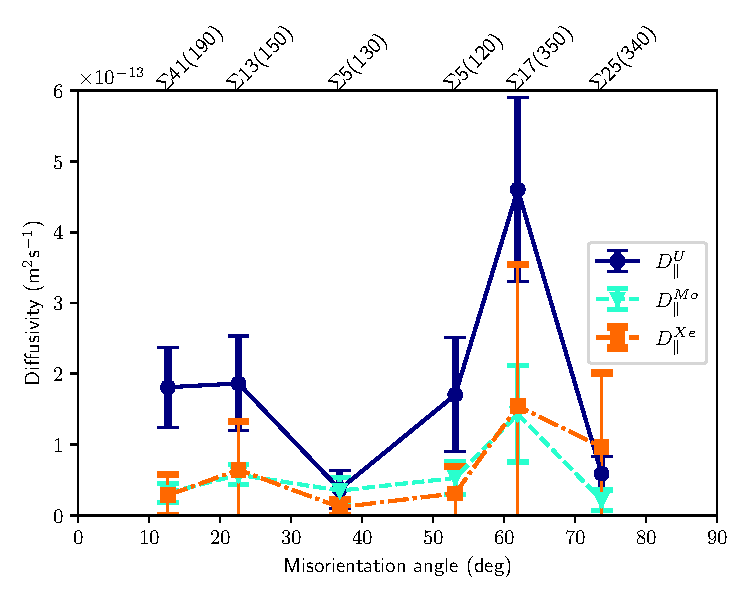
\includegraphics[width=\textwidth]{DvsTilt_600K.pdf}
    \end{subfigure}
    \begin{subfigure}{0.49\textwidth}
        \centering
        \caption{}
        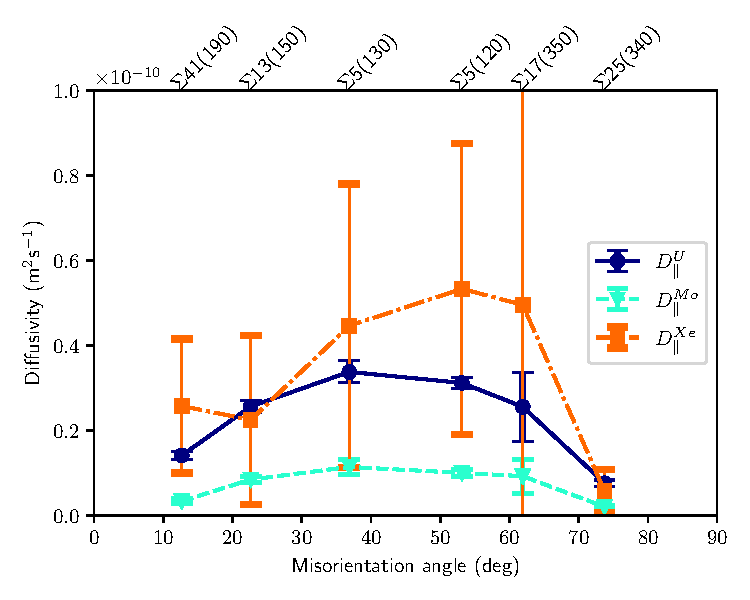
\includegraphics[width=\textwidth]{DvsTilt_1200K.pdf}
    \end{subfigure}
\caption{\DIFaddFL{Diffusivities of U, Mo, and Xe with respect to the misorientation angle in $\gamma$U-10Mo at (a) 600 K, and (b) 1200 K.}}
\label{fig:dvstilt}
\end{figure}

%DIF > \begin{table}[!ht]
%DIF > \centering
%DIF > \caption{Grain boundary energies (in Jm$^{-2}$) of $\gamma$U-10Mo symmetric tilt grain boundaries at 600 K and 1200 K from Beeler et al.
%DIF > \cite{beeler2018}.}
%DIF > \label{tab:gbe_corr}
%DIF > \begin{tabular}{ccc}
%DIF > \toprule
%DIF > GB plane & 600 K & 1200 K \\
%DIF > \midrule
%DIF > \{190\} & 0.53 & 0.61 \\
%DIF > \{150\} & 0.57 & 0.70 \\
%DIF > \{130\} & 0.55 & 0.68 \\
%DIF > \{120\} & 0.57 & 0.73 \\
%DIF > \bottomrule
%DIF > \end{tabular}
%DIF > \end{table}

\DIFadd{At 600 K, there is no apparent relation of the diffusivity with the misorientation angle. The minima occur for the }\DIFaddend \{130\DIFdelbegin \DIFdel{\} GB. The symmetric tilt \{130}\DIFdelend \} \DIFdelbegin \DIFdel{GB might be a special boundary and additional simulations would likely be required to verify the exception. At high temperatures, the amount of misorientation affects both LAGBs and HAGBs. The }\DIFdelend \DIFaddbegin \DIFadd{and \{340\} GBs, with the maximum at the \{350\}. However, at 1200 K, the misorientation angle does show an effect on the diffusivities. In general, the }\DIFaddend greater the misorientation \DIFaddbegin \DIFadd{(closer to 45$^{\circ}$)}\DIFaddend , the greater the diffusivity. \DIFdelbegin \DIFdel{It is to be emphasized that misorientation }\DIFdelend \DIFaddbegin \DIFadd{This might mean high temperature allows some GB structures to use additional diffusional pathways. Utilizing the GB energies calculated at 1200 K in Figure \ref{fig:gbe} and Table \ref{tab:gbe}, one can investigate a potential correlation between the GB energies and the diffusivities. This data is plotted in Figure \ref{fig:DvsGBE} and indicates that there is not a statistically significant correlation. Data from GBs at 600 K \cite{beeler2018} are also analyzed to explore temperature effects, but again, no clear patterns could be identified. Thus, while there is a dependence of diffusion on the GB orientation, there are no consistent trends with respect to either the misorientation angle or the GB energy across the entire temperature spectrum analyzed.
}

\FloatBarrier
\section{\DIFadd{Discussion}}

\subsection{\DIFadd{Anisotropic nature of diffusion}}

\DIFadd{GBs can be differentiated into either low-angle GBs (LAGBs) or high-angle GBs (HAGBs) based on the presence of discrete lattice dislocations in the structure \cite{winning2010}. The transition from LAGB to HAGB happens between 10$^{\circ}$ and 20$^{\circ}$. Even around 20$^{\circ}$, some GBs might have discernible single dislocations \cite{winning2005}. Since $\gamma$U-Mo has a bcc structure, having a 90$^{\circ}$ tilt means it is a perfect lattice without any GBs. Also, the misorientation }\DIFaddend angles $\theta$ and \DIFdelbegin \DIFdel{$90-\theta$ }\DIFdelend \DIFaddbegin \DIFadd{$(\theta+90^{\circ})$ }\DIFaddend are the same because of the inherent symmetry in bcc structures. \DIFaddbegin \DIFadd{Among the examined symmetric tilt GBs in this work, \{190\} and \{340\} can be considered LAGBs and \{150\}, \{130\}, \{120\}, and \{350\} HAGBs.
}\DIFaddend 

\DIFaddbegin \DIFadd{Figure \ref{fig:ratio} depicts the ratio $D^i_{\parallel} / D^i_{\perp}$ for symmetric tilt GBs in $\gamma$U-10Mo where $i =$ U, Mo, or Xe. The solid black line at $D^i_{\parallel} / D^i_{\perp} = 1$ represents isotropic GB diffusion. For all the symmetric tilt HAGBs, the diffusion is closer to the isotropic behavior. The symmetric tilt \{190\} LAGB shows highly anisotropic GB diffusion, especially for U GB diffusion. The symmetric tilt \{340\} LAGB also shows anisotropic behavior but only at lower temperatures. At high temperatures, the diffusion behavior of the \{340\} GB is almost isotropic, similar to other HAGBs. Some anisotropy is expected even in HAGBs \cite{mishin1997}.
}

\DIFaddend \begin{figure}[!ht]
    \centering
    \begin{subfigure}{0.49\textwidth}
        \centering
        \caption{}
        \DIFdelbeginFL %DIFDELCMD < 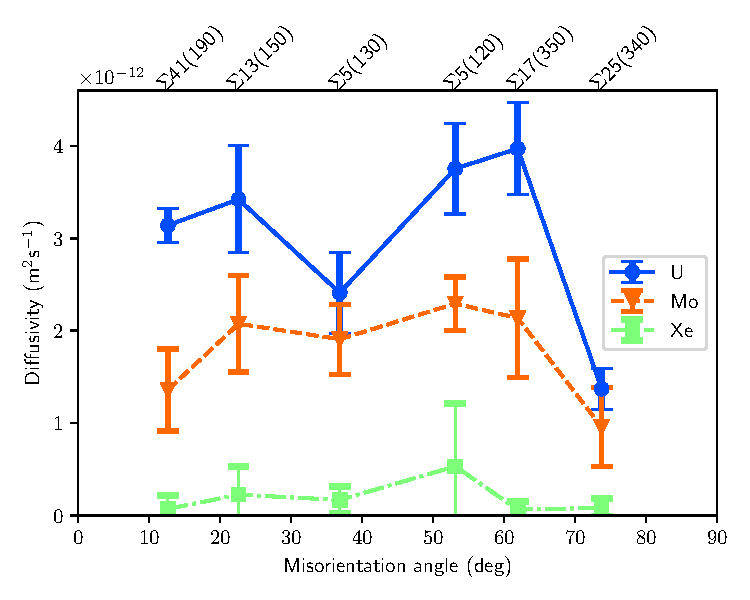
\includegraphics[width=\textwidth]{DvsTilt_10mo_2.pdf}
%DIFDELCMD <     %%%
\DIFdelendFL \DIFaddbeginFL 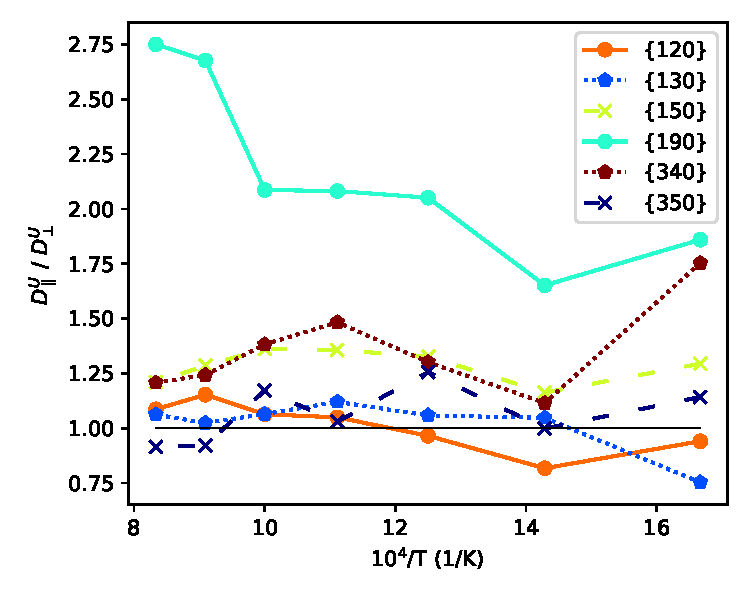
\includegraphics[width=\textwidth]{ratio_U.pdf}
    \DIFaddendFL \end{subfigure}
    \begin{subfigure}{0.49\textwidth}
        \centering
        \caption{}
        \DIFdelbeginFL %DIFDELCMD < 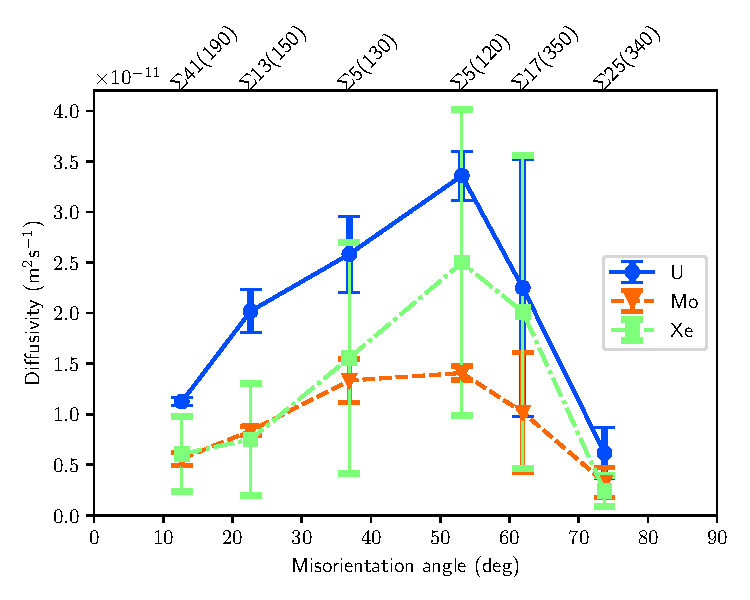
\includegraphics[width=\textwidth]{DvsTilt_10mo.pdf}
%DIFDELCMD <     %%%
\DIFdelendFL \DIFaddbeginFL 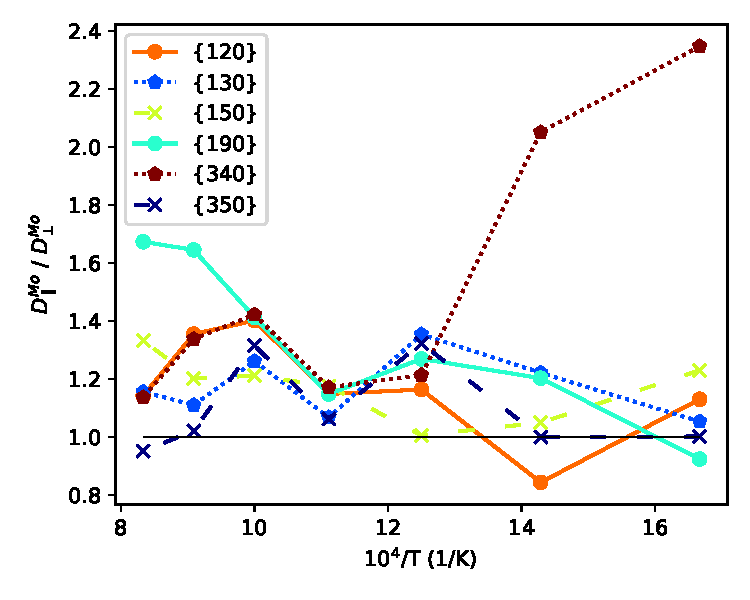
\includegraphics[width=\textwidth]{ratio_Mo.pdf}
    \DIFaddendFL \end{subfigure}
    \DIFdelbeginFL %DIFDELCMD < \caption{%
{%DIFAUXCMD
\DIFdelFL{Diffusivities for U, Mo, and Xe with respect to misorientation angles for $\gamma$U-10Mo at (a) 800 K, and (b) 1200 K.}}
%DIFAUXCMD
%DIFDELCMD < \label{fig:dvstilt}
%DIFDELCMD < %%%
\DIFdelendFL \DIFaddbeginFL \begin{subfigure}{0.49\textwidth}
        \centering
        \caption{}
        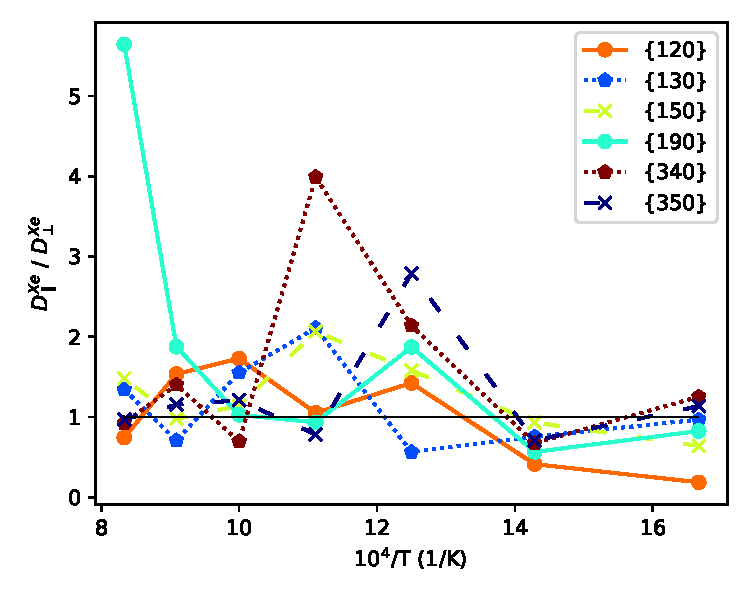
\includegraphics[width=\textwidth]{ratio_Xe.pdf}
    \end{subfigure}
\caption{\DIFaddFL{Ratios of the diffusion coefficients parallel to the tilt axis to the diffusion coefficients perpendicular to the tilt axis of (a) U, (b) Mo, and (c) Xe in the symmetric tilt grain boundaries in $\gamma$U-10Mo.}}
\label{fig:ratio}
\DIFaddendFL \end{figure}

\DIFdelbegin \DIFdel{There do not appear to be any species-specific trends from the misorientation angle, as all species generally diffuse faster at higher temperatures, and tend to diffuse slightly faster with misorientation angles between 30$^{\circ}$ and 65$^{\circ}$.
For all examined misorientation angles at low temperatures, the following trend seems to be true in general:
}%DIFDELCMD < \begin{align}
%DIFDELCMD < 	D_{gb}^U > D_{gb}^{Mo} > D_{gb}^{Xe}
%DIFDELCMD < \end{align}
%DIFDELCMD < %%%
\DIFdel{However, this trend tends to break down at high temperatures where D$_{gb}^{Xe}$ becomes comparable to that for U and Mo. It can also be seen that the Xe diffusion coefficients have a larger relative variance compared to the other two species. This is expected since we only compute properties from the diffusion of 2 Xe atoms per simulation.
In contrast, we have thousands of U and Mo atoms per simulation.
}%DIFDELCMD < 

%DIFDELCMD < \FloatBarrier
%DIFDELCMD < %%%
\section{\DIFdel{Discussion}}
%DIFAUXCMD
\addtocounter{section}{-1}%DIFAUXCMD
%DIFDELCMD < 

%DIFDELCMD < %%%
\subsection{\DIFdel{Nature of diffusion}}
%DIFAUXCMD
\addtocounter{subsection}{-1}%DIFAUXCMD
%DIFDELCMD < 

%DIFDELCMD < %%%
\DIFdel{GBs can be interpreted as collections of dislocations and a pure tilt GB }\DIFdelend \DIFaddbegin \DIFadd{A symmetric tilt LAGB }\DIFaddend is essentially an array of parallel edge dislocations. Analysis of the atomistic simulations performed in this work reveals dislocation pipe diffusion \DIFdelbegin \DIFdel{in symmetric tilt LAGBs, and this diffusion }\DIFdelend \DIFaddbegin \DIFadd{parallel to the tilt axis in the symmetric tilt \{190\} GB, and diffusion in this GB }\DIFaddend is mostly one-dimensional\DIFdelbegin \DIFdel{where the diffusion pipes are parallel to the tilt axis}\DIFdelend . The atomic trajectories in a cross-sectional GB view and the directional MSDs of the symmetric tilt \{190\} \DIFaddbegin \DIFadd{GB system }\DIFaddend are provided in Figure \ref{fig:190}. Subfigures \ref{fig:190}(a) and \ref{fig:190}(b) are at 700 K, and \ref{fig:190}(c) and \ref{fig:190}(d) are at 1100 K. The cross-sections reveal the diffusion pipes. Diffusion outside these pipes is not prominent even if the atoms are within the GB plane. \DIFdelbegin \DIFdel{This explains why the effective GB width as defined in section \ref{sec:res1} can sometimes be less than the lattice parameter, as not all atoms at the GB are participating in the diffusion. }\DIFdelend The MSDs in the direction perpendicular to the GB plane (y-axis), and in the direction perpendicular to the tilt axis but parallel to the GB plane (x-axis) are similar in magnitude. Thus, it can be stated that the diffusion in the symmetric tilt \{190\} GB is primarily happening in the direction of the tilt axis.

\begin{figure}[!ht]
\centering
	\begin{subfigure}{0.49\textwidth}
		\centering
		\caption{}
		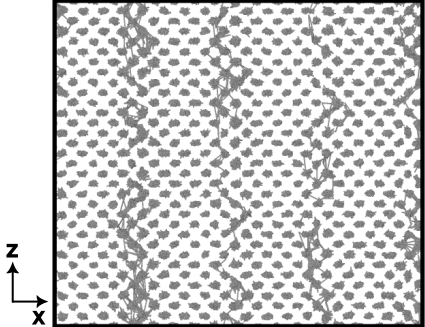
\includegraphics[height=5cm]{190at700cs.png}
	\end{subfigure}
	\begin{subfigure}{0.49\textwidth}
		\centering
		\caption{}
		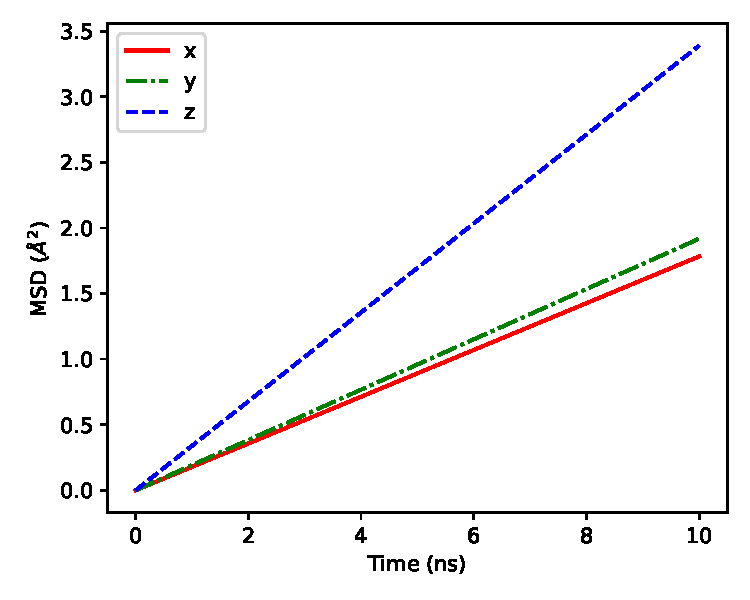
\includegraphics[height=5cm]{190at700xyz.pdf}
	\end{subfigure}
    \par\medskip
	\begin{subfigure}{0.49\textwidth}
		\centering
		\caption{}
		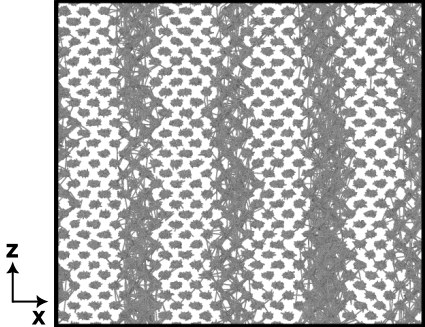
\includegraphics[height=5cm]{190at1100cs.png}
	\end{subfigure}
	\begin{subfigure}{0.49\textwidth}
		\centering
		\caption{}
		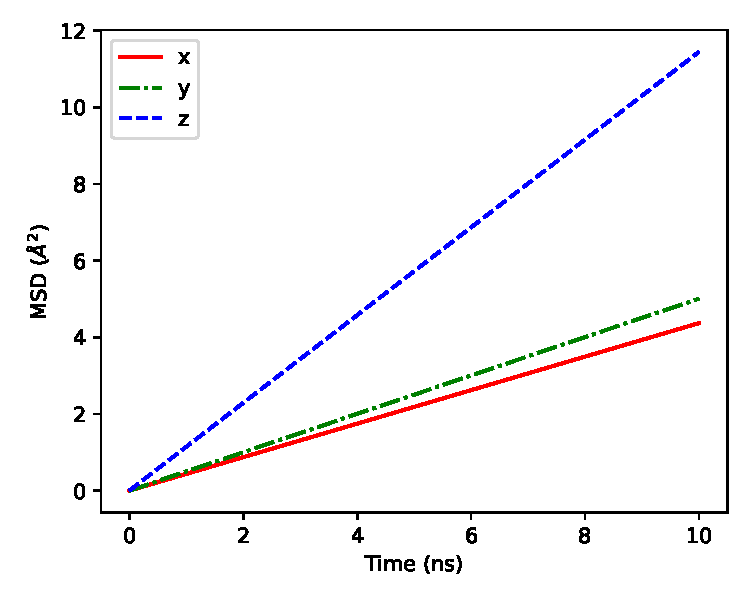
\includegraphics[height=5cm]{190at1100xyz.pdf}
	\end{subfigure}
\caption{\DIFdelbeginFL \DIFdelFL{Atomic trajectory lines in }\DIFdelendFL \DIFaddbeginFL \DIFaddFL{Cross-sectional view of }\DIFaddendFL the \DIFdelbeginFL \DIFdelFL{GB cross sections }\DIFdelendFL \DIFaddbeginFL \DIFaddFL{atomic trajectories }\DIFaddendFL at (a) 700 K and (c) 1100 K, and the \DIFdelbeginFL \DIFdelFL{MSD }\DIFdelendFL \DIFaddbeginFL \DIFaddFL{MSDs }\DIFaddendFL at (b) 700 K and (d) 1100 K for the symmetric tilt \{190\} grain boundary.}
\label{fig:190}
\end{figure}

Figure \ref{fig:130} displays the atomic trajectories and the directional MSDs for the symmetric tilt \{130\} \DIFdelbegin \DIFdel{GB}\DIFdelend \DIFaddbegin \DIFadd{HAGB}\DIFaddend . Contrary to the \{190\} system, the diffusion in \{130\} is two-dimensional \DIFdelbegin \DIFdel{. The }\DIFdelend \DIFaddbegin \DIFadd{and the }\DIFaddend diffusion on the GB plane does not have any directional preference\DIFdelbegin \DIFdel{in this case}\DIFdelend . This is true for \DIFdelbegin \DIFdel{most }\DIFdelend \DIFaddbegin \DIFadd{all }\DIFaddend HAGBs. For some configurations, such as the \{340\} \DIFdelbegin \DIFdel{system }\DIFdelend \DIFaddbegin \DIFadd{LAGB }\DIFaddend (misorientation angle of 16.3\DIFdelbegin \DIFdel{degrees}\DIFdelend \DIFaddbegin \DIFadd{$^{\circ}$}\DIFaddend ), the diffusion behavior can be somewhere in between. In \DIFdelbegin \DIFdel{those cases}\DIFdelend \DIFaddbegin \DIFadd{this case}\DIFaddend , the diffusion parallel to the tilt axis is significantly stronger than the diffusion perpendicular to the tilt axis (and parallel to the GB plane), which in turn is significantly stronger than the diffusion perpendicular to the GB plane. Thus, \DIFdelbegin \DIFdel{while the magnitude of diffusion is only marginally dependent upon the orientation of the GBs, the }\DIFdelend \DIFaddbegin \DIFadd{the }\DIFaddend underlying nature of diffusion \DIFdelbegin \DIFdel{on }\DIFdelend \DIFaddbegin \DIFadd{in }\DIFaddend symmetric tilt GBs can be substantially different, including 1-D or anisotropic effects, and such behaviors become more prevalent for \DIFdelbegin \DIFdel{LAGBs}\DIFdelend \DIFaddbegin \DIFadd{low-angle GBs}\DIFaddend .

\begin{figure}[!ht]
\centering
	\begin{subfigure}{0.49\textwidth}
		\centering
		\caption{}
		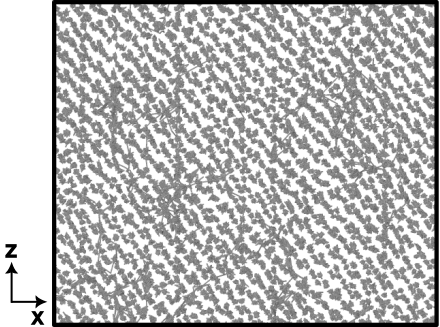
\includegraphics[height=5cm]{130at700cs.png}
	\end{subfigure}
	\begin{subfigure}{0.49\textwidth}
		\centering
		\caption{}
		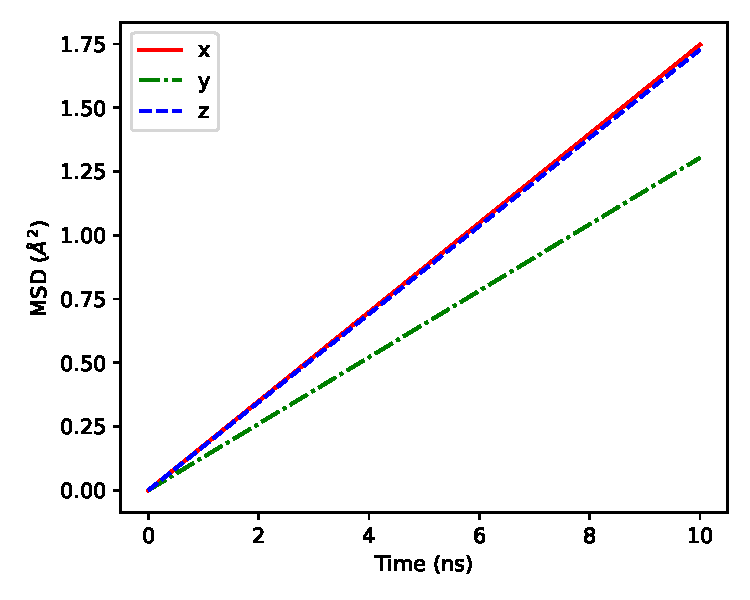
\includegraphics[height=5cm]{130at700xyz.pdf}
	\end{subfigure}
    \par\medskip
	\begin{subfigure}{0.49\textwidth}
		\centering
		\caption{}
		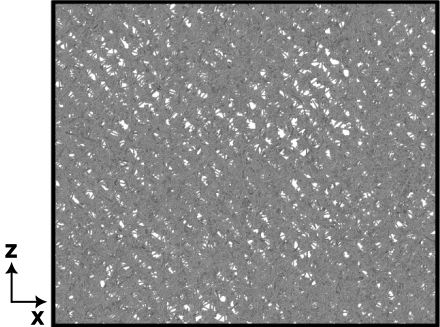
\includegraphics[height=5cm]{130at1100cs.png}
	\end{subfigure}
	\begin{subfigure}{0.49\textwidth}
		\centering
		\caption{}
		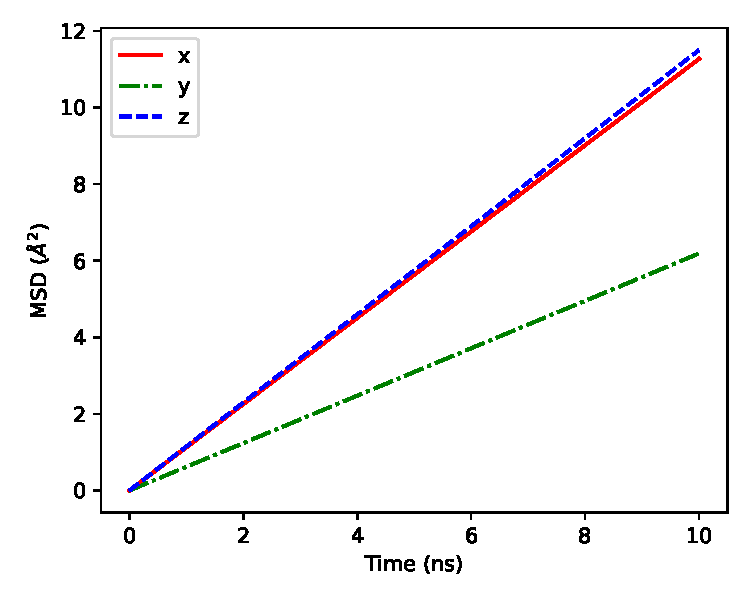
\includegraphics[height=5cm]{130at1100xyz.pdf}
	\end{subfigure}
\caption{\DIFdelbeginFL \DIFdelFL{Atomic trajectory lines in }\DIFdelendFL \DIFaddbeginFL \DIFaddFL{Cross-sectional view of }\DIFaddendFL the \DIFdelbeginFL \DIFdelFL{GB cross sections }\DIFdelendFL \DIFaddbeginFL \DIFaddFL{atomic trajectories }\DIFaddendFL at (a) 700 K and (c) 1100 K, and the \DIFdelbeginFL \DIFdelFL{MSD }\DIFdelendFL \DIFaddbeginFL \DIFaddFL{MSDs }\DIFaddendFL at (b) 700 K and (d) 1100 K for the symmetric tilt \{130\} grain boundary.}
\label{fig:130}
\end{figure}


\FloatBarrier
\subsection{Two diffusion regimes based on temperature}

The \DIFdelbegin \DIFdel{diffusion coefficients of }\DIFdelend \DIFaddbegin \DIFadd{GB diffusion coefficients in }\DIFaddend $\gamma$U-Mo roughly follow the Arrhenius equation, but not exactly. The Arrhenius plot displays concavity for all configurations, indicating the possibility of sub-Arrhenius behavior. Similar behavior has been observed in U$_3$Si$_2$ fuel by Cooper et al. \cite{cooper2021} \DIFdelbegin \DIFdel{, }\DIFdelend but was neglected. Figure \ref{fig:2reg} shows the same data as in Figure \ref{fig:comp}, but separated into two different regimes: a high-temperature regime from 900 K to 1200 K and a low-temperature regime from 600 K to 800 K. A GB diffusion study by Suzuki et al. \cite{suzuki2005} describes this as heterophase fluctuations. The Arrhenius plots for Cu GB diffusion from Suzuki also show concavity, and they theorized this as a local melting event, where small embryos of liquid are supposed to exist for a short time before crystallizing into an ordered GB structure.

\begin{figure}[!ht]
\DIFaddbeginFL \begin{subfigure}{0.49\textwidth}
	\DIFaddendFL \centering
	\DIFdelbeginFL %DIFDELCMD < 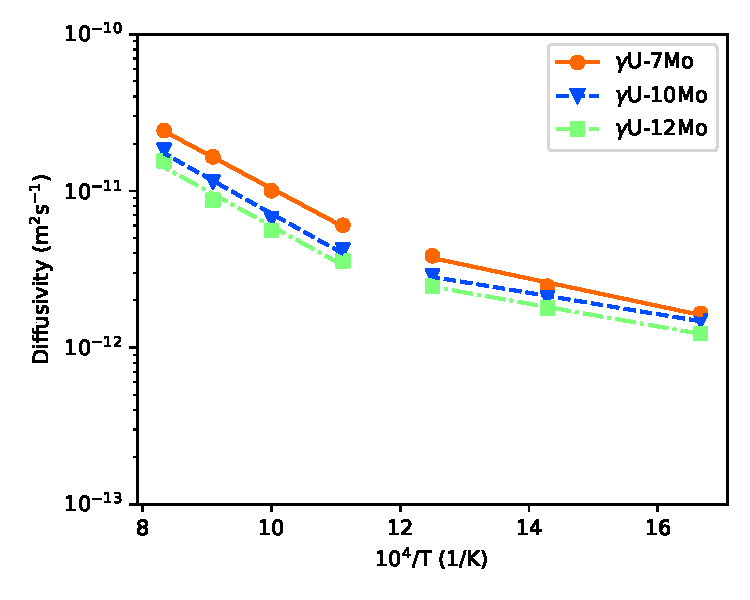
\includegraphics[width=0.60\textwidth]{2reg.pdf}
%DIFDELCMD < %%%
\DIFdelendFL \caption{\DIFdelbeginFL \DIFdelFL{Arrehenius fits to two diffusion regimes.}\DIFdelendFL }
	\DIFaddbeginFL 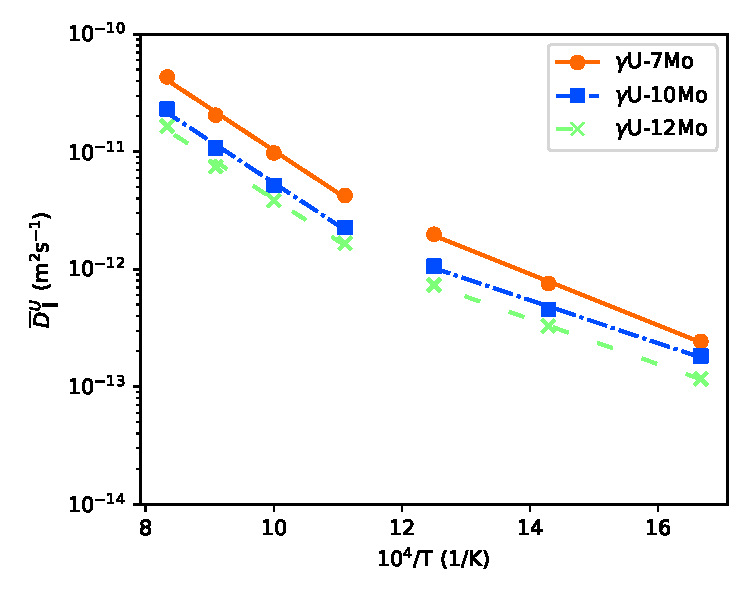
\includegraphics[width=\textwidth]{2reg_U_Dz.pdf}
\end{subfigure}
\begin{subfigure}{0.49\textwidth}
	\centering
	\caption{}
	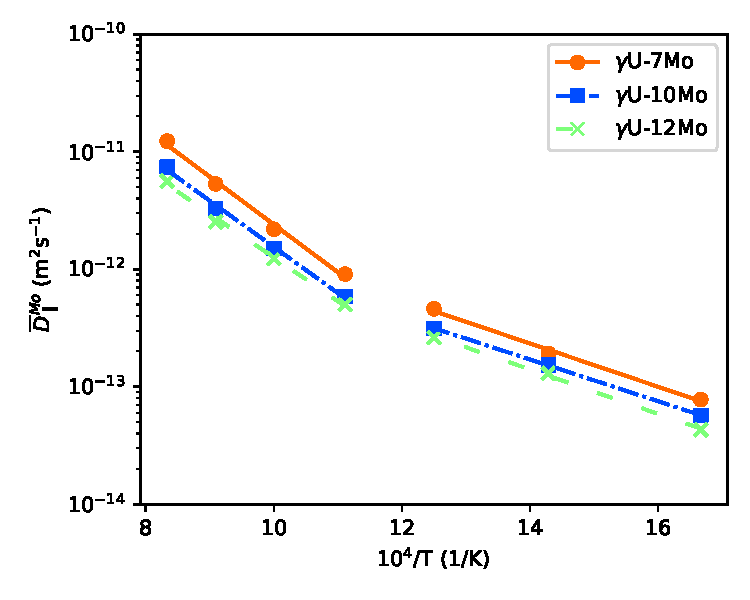
\includegraphics[width=\textwidth]{2reg_Mo_Dz.pdf}
\end{subfigure}
\caption{\DIFaddFL{Orientation-averaged grain boundary diffusion coefficients of (a) U and (b) Mo parallel to the tilt axis for $\gamma$U-7Mo, $\gamma$U-10Mo, and $\gamma$U-12Mo with Arrhenius fits to the two diffusion regimes.}}
\DIFaddendFL \label{fig:2reg}
\end{figure}

Arrhenius fits are thus applied separately for these two temperature regimes observed in Figure \ref{fig:2reg}, and prefactors and activation energies for these two regimes are provided in \DIFdelbegin \DIFdel{Tables \ref{tab:compArrHigh} and \ref{tab:compArrLow}}\DIFdelend \DIFaddbegin \DIFadd{Table \ref{tab:2reg}}\DIFaddend . The activation energy for \DIFdelbegin \DIFdel{total GB diffusion is 0.457 eV for U-10Mo at high temperatures}\DIFdelend \DIFaddbegin \DIFadd{U GB diffusion in $\gamma$U-10Mo is 0.36 eV in the low-temperature regime and 0.71 in the high-temperature regime}\DIFaddend , which is \DIFdelbegin \DIFdel{3.4 times higher than the activation energy at low temperatures(0.135 eV). }\DIFdelend \DIFaddbegin \DIFadd{almost double the value at low temperatures. Although the activation energy for Mo GB diffusion is a little higher than that of U GB diffusion at high temperatures, the overall trend is similar. The effect of composition on the activation energies is minimal. }\DIFaddend We suggest the use of Arrhenius fits that are based on the two temperature regimes, e.g., to calculate the diffusion coefficient at 300 K, the low-temperature fit should be used. \DIFaddbegin \DIFadd{Linear interpolation can be used for the temperature range 800 K - 900 K.
}\DIFaddend 

\begin{table}[!ht]
\centering
\caption{Prefactors and activation energies for the \DIFdelbeginFL \DIFdelFL{Arrhrenius }\DIFdelendFL \DIFaddbeginFL \DIFaddFL{Arrhenius }\DIFaddendFL equation fits \DIFdelbeginFL \DIFdelFL{for various compositions }\DIFdelendFL \DIFaddbeginFL \DIFaddFL{to $\overline{D}^{i}_{\parallel}$ ($i=$ U or Mo) }\DIFaddendFL in \DIFaddbeginFL \DIFaddFL{$\gamma$U-7Mo, $\gamma$U-10Mo, and $\gamma$U-12Mo for }\DIFaddendFL the \DIFdelbeginFL \DIFdelFL{high-temperature regime}\DIFdelendFL \DIFaddbeginFL \DIFaddFL{two different temperature regimes}\DIFaddendFL . \DIFaddbeginFL \DIFaddFL{$D_0$ is in m$^2$s$^{-1}$ and $E_a$ is in eV.}\DIFaddendFL }
\DIFdelbeginFL %DIFDELCMD < \label{tab:compArrHigh}
%DIFDELCMD < \begin{tabular}{lllllll}
%DIFDELCMD < %%%
\DIFdelendFL 
\DIFaddbeginFL \label{tab:2reg}
\begin{tabular}{ccllll}
\DIFaddendFL 
\toprule
Composition & \DIFdelbeginFL \DIFdelFL{$D_{0,gb}^U$      }\DIFdelendFL \DIFaddbeginFL \DIFaddFL{Temp.
	}\DIFaddendFL & \DIFdelbeginFL \DIFdelFL{$E_{a,gb}^U$
	    }\DIFdelendFL \DIFaddbeginFL \DIFaddFL{$D_{0}^U$      }\DIFaddendFL & \DIFdelbeginFL \DIFdelFL{$D_{0,gb}^{Mo}$   }\DIFdelendFL \DIFaddbeginFL \DIFaddFL{$E_{a}^U$
	}\DIFaddendFL & \DIFdelbeginFL \DIFdelFL{$E_{a,gb}^{Mo}$
	    }\DIFdelendFL \DIFaddbeginFL \DIFaddFL{$D_{0}^{Mo}$   }\DIFaddendFL & \DIFdelbeginFL \DIFdelFL{$D_{0,gb}^{Tot}$  }%DIFDELCMD < & %%%
\DIFdelFL{$E_{a,gb}^{Tot}$ }\DIFdelendFL \DIFaddbeginFL \DIFaddFL{$E_{a}^{Mo}$ }\DIFaddendFL \\
\midrule
\DIFdelbeginFL \DIFdelFL{$\gamma$U-7Mo  }\DIFdelendFL \DIFaddbeginFL \multirow{2}{*}{ $\gamma$U-7Mo }
	\DIFaddendFL & \DIFdelbeginFL \DIFdelFL{1.76 $\times 10^{-9}$ }\DIFdelendFL \DIFaddbeginFL \DIFaddFL{600 K - 800 K
	}\DIFaddendFL & \DIFdelbeginFL \DIFdelFL{0.438 }\DIFdelendFL \DIFaddbeginFL \DIFaddFL{1.03 $\times 10^{-09}$ }\DIFaddendFL & \DIFdelbeginFL \DIFdelFL{9.04 $\times 10^{-10}$
	       }\DIFdelendFL \DIFaddbeginFL \DIFaddFL{0.433
	}\DIFaddendFL & \DIFdelbeginFL \DIFdelFL{0.455 }\DIFdelendFL \DIFaddbeginFL \DIFaddFL{8.87 $\times 10^{-11}$ }\DIFaddendFL & \DIFdelbeginFL \DIFdelFL{1.61 $\times 10^{-9}$ }%DIFDELCMD < & %%%
\DIFdelFL{0.435  }\DIFdelendFL \DIFaddbeginFL \DIFaddFL{0.366 }\DIFaddendFL \\
	\DIFdelbeginFL \DIFdelFL{$\gamma$U-10Mo }\DIFdelendFL & \DIFdelbeginFL \DIFdelFL{1.76 $\times 10^{-9}$ }\DIFdelendFL \DIFaddbeginFL \DIFaddFL{900 K - 1200 K
	}\DIFaddendFL & \DIFdelbeginFL \DIFdelFL{0.468 }\DIFdelendFL \DIFaddbeginFL \DIFaddFL{4.10 $\times 10^{-08}$ }\DIFaddendFL & \DIFdelbeginFL \DIFdelFL{4.47 $\times 10^{-10}$
	       }\DIFdelendFL \DIFaddbeginFL \DIFaddFL{0.715
	}\DIFaddendFL & \DIFdelbeginFL \DIFdelFL{0.412 }\DIFdelendFL \DIFaddbeginFL \DIFaddFL{2.77 $\times 10^{-08}$ }\DIFaddendFL & \DIFdelbeginFL \DIFdelFL{1.45 $\times 10^{-9}$ }%DIFDELCMD < & %%%
\DIFdelFL{0.457  }\DIFdelendFL \DIFaddbeginFL \DIFaddFL{0.806 }\vspace{0.2cm } \DIFaddendFL \\
\DIFdelbeginFL \DIFdelFL{$\gamma$U-12Mo }\DIFdelendFL \DIFaddbeginFL \multirow{2}{*}{ $\gamma$U-10Mo }
	\DIFaddendFL & \DIFdelbeginFL \DIFdelFL{1.35 $\times 10^{-9}$ }\DIFdelendFL \DIFaddbeginFL \DIFaddFL{600 K - 800 K
	}\DIFaddendFL & \DIFdelbeginFL \DIFdelFL{0.460 }%DIFDELCMD < & %%%
\DIFdelFL{3.13 }\DIFdelendFL \DIFaddbeginFL \DIFaddFL{1.96 }\DIFaddendFL $\times 10^{-10}$ & \DIFdelbeginFL \DIFdelFL{0.390 }\DIFdelendFL \DIFaddbeginFL \DIFaddFL{0.362
	}\DIFaddendFL & \DIFdelbeginFL \DIFdelFL{1.06 $\times 10^{-9}$ }\DIFdelendFL \DIFaddbeginFL \DIFaddFL{5.26 $\times 10^{-11}$ }\DIFaddendFL & \DIFdelbeginFL \DIFdelFL{0.447  }\DIFdelendFL \DIFaddbeginFL \DIFaddFL{0.353 }\DIFaddendFL \\
	\DIFdelbeginFL %DIFDELCMD < \bottomrule
%DIFDELCMD < \end{tabular}
%DIFDELCMD < \end{table}
%DIFDELCMD < 

%DIFDELCMD < \begin{table}[!ht]
%DIFDELCMD < \centering
%DIFDELCMD < %%%
%DIFDELCMD < \caption%
{%DIFAUXCMD
\DIFdelFL{Prefactors and activation energies for the Arrhrenius equation fits for various compositions in the low-temperature regime.}}
%DIFAUXCMD
%DIFDELCMD < \label{tab:compArrLow}
%DIFDELCMD < \begin{tabular}{lllllll}
%DIFDELCMD < \toprule
%DIFDELCMD < %%%
\DIFdelFL{Composition }\DIFdelendFL & \DIFdelbeginFL \DIFdelFL{$D_{0,gb}^U$      }\DIFdelendFL \DIFaddbeginFL \DIFaddFL{900 K - 1200 K
	}\DIFaddendFL & \DIFdelbeginFL \DIFdelFL{$E_{a,gb}^U$
	    }\DIFdelendFL \DIFaddbeginFL \DIFaddFL{2.10 $\times 10^{-08}$ }\DIFaddendFL & \DIFdelbeginFL \DIFdelFL{$D_{0,gb}^{Mo}$   }\DIFdelendFL \DIFaddbeginFL \DIFaddFL{0.712
	}\DIFaddendFL & \DIFdelbeginFL \DIFdelFL{$E_{a,gb}^{Mo}$
	    }\DIFdelendFL \DIFaddbeginFL \DIFaddFL{1.31 $\times 10^{-08}$ }\DIFaddendFL & \DIFdelbeginFL \DIFdelFL{$D_{0,gb}^{Tot}$  }%DIFDELCMD < & %%%
\DIFdelFL{$E_{a,gb}^{Tot}$ }\DIFdelendFL \DIFaddbeginFL \DIFaddFL{0.779 }\vspace{0.2cm } \DIFaddendFL \\
\DIFdelbeginFL %DIFDELCMD < \midrule
%DIFDELCMD < %%%
\DIFdelFL{$\gamma$U-7Mo  }\DIFdelendFL \DIFaddbeginFL \multirow{2}{*}{ $\gamma$U-12Mo }
	\DIFaddendFL & \DIFdelbeginFL \DIFdelFL{5.08 $\times 10^{-11}$ }\DIFdelendFL \DIFaddbeginFL \DIFaddFL{600 K - 800 K
	}\DIFaddendFL & \DIFdelbeginFL \DIFdelFL{0.177 }\DIFdelendFL \DIFaddbeginFL \DIFaddFL{1.81 $\times 10^{-10}$ }\DIFaddendFL & \DIFdelbeginFL \DIFdelFL{1.12 $\times 10^{-11}$
	       }\DIFdelendFL \DIFaddbeginFL \DIFaddFL{0.380
	}\DIFaddendFL & \DIFdelbeginFL \DIFdelFL{0.119 }%DIFDELCMD < & %%%
\DIFdelFL{4.61 }\DIFdelendFL \DIFaddbeginFL \DIFaddFL{6.17 }\DIFaddendFL $\times 10^{-11}$ & \DIFdelbeginFL \DIFdelFL{0.173  }\DIFdelendFL \DIFaddbeginFL \DIFaddFL{0.375 }\DIFaddendFL \\
	\DIFdelbeginFL \DIFdelFL{$\gamma$U-10Mo }\DIFdelendFL & \DIFdelbeginFL \DIFdelFL{2.16 $\times 10^{-11}$ }\DIFdelendFL \DIFaddbeginFL \DIFaddFL{900 K - 1200 K}\DIFaddendFL & \DIFdelbeginFL \DIFdelFL{0.137 }\DIFdelendFL \DIFaddbeginFL \DIFaddFL{1.33 $\times 10^{-08}$ }\DIFaddendFL & \DIFdelbeginFL \DIFdelFL{1.03 $\times 10^{-11}$    }\DIFdelendFL \DIFaddbeginFL \DIFaddFL{0.700}\DIFaddendFL & \DIFdelbeginFL \DIFdelFL{0.120 }\DIFdelendFL \DIFaddbeginFL \DIFaddFL{6.62 $\times 10^{-09}$ }\DIFaddendFL & \DIFdelbeginFL \DIFdelFL{2.01 $\times 10^{-11}$ }%DIFDELCMD < & %%%
\DIFdelFL{0.135  }\DIFdelendFL \DIFaddbeginFL \DIFaddFL{0.738 }\DIFaddendFL \\
\bottomrule
\DIFdelbeginFL \DIFdelFL{$\gamma$U-12Mo }%DIFDELCMD < & %%%
\DIFdelFL{2.12 $\times 10^{-11}$ }%DIFDELCMD < & %%%
\DIFdelFL{0.145 }%DIFDELCMD < & %%%
\DIFdelFL{1.11 $\times 10^{-11}$ 	       }%DIFDELCMD < & %%%
\DIFdelFL{0.129 }%DIFDELCMD < & %%%
\DIFdelFL{1.96 $\times 10^{-11}$ }%DIFDELCMD < & %%%
\DIFdelFL{0.143  }%DIFDELCMD < \\

%DIFDELCMD < %%%
\DIFdelendFL

\end{tabular}
\end{table}

These regimes \DIFdelbegin \DIFdel{may be due to }\DIFdelend \DIFaddbegin \DIFadd{might exist due to the }\DIFaddend different modes of diffusion that only get enabled at high temperatures, with the transition between the two \DIFdelbegin \DIFdel{diffusion }\DIFdelend regimes occurring at \DIFdelbegin \DIFdel{800-900 K }\DIFdelend \DIFaddbegin \DIFadd{800 K - 900 K }\DIFaddend for this system. With additional thermal energy, given a fixed migration barrier, higher temperatures are more likely to overcome the energy barrier and induce diffusion. Given that 1) more atoms are participating in the diffusional process as temperature increases (Figure \DIFdelbegin \DIFdel{\ref{fig:atomVsT}}\DIFdelend \DIFaddbegin \DIFadd{\ref{fig:delta}}\DIFaddend ), 2) diffusional pathways appear to become more varied at increasing temperature (Figure \ref{fig:130}), and 3) that the high-temperature diffusion regime exhibits a higher activation energy (Figure \ref{fig:2reg}), the assumption that increased temperature opens higher energy diffusional pathways seems reasonable. This may be an alternate way of viewing the same phenomena identified in Suzuki \cite{suzuki2005} and denoted as heterophase fluctuations. 


\FloatBarrier
\section{Conclusions}

In the present work, MD simulations are performed using an ADP potential to compute \DIFaddbegin \DIFadd{the }\DIFaddend GB diffusion coefficients \DIFaddbegin \DIFadd{of U, Mo, and Xe }\DIFaddend in $\gamma$U-Mo alloys \cite{starikov2018}. First, \DIFdelbegin \DIFdel{a way to distinguish the GB atoms is developed by individually identifying atoms that are participating in the GB diffusion process}\DIFdelend \DIFaddbegin \DIFadd{the GB region is identified by locating the lattice point jumps of atoms using the atomic trajectories}\DIFaddend . It is observed that the \DIFdelbegin \DIFdel{number of GB atoms increases almost exponentially }\DIFdelend \DIFaddbegin \DIFadd{GB width increases almost linearly from around 6 \r{A} to around 12 \r{A} }\DIFaddend with temperature in the range \DIFdelbegin \DIFdel{of }\DIFdelend 600 K - 1200 K. The \DIFdelbegin \DIFdel{MSD of the GB atoms is }\DIFdelend \DIFaddbegin \DIFadd{MSDs of the U, Mo, and Xe atoms are }\DIFaddend then used to calculate the GB diffusivities of \DIFaddbegin \DIFadd{the species in }\DIFaddend several $\gamma$U-Mo alloys ($\gamma$U-7Mo, $\gamma$U-10Mo, and $\gamma$U-12Mo) as a function of temperature and misorientation angle. \DIFdelbegin \DIFdel{GB diffusivities of U, Mo, and Xe are computed along with total GB diffusivity. The total GB diffusion is }\DIFdelend \DIFaddbegin \DIFadd{The GB diffusion coefficients are }\DIFaddend typically on the order of \DIFdelbegin \DIFdel{$10^{-12}$ }\DIFdelend \DIFaddbegin \DIFadd{$10^{-14}$ }\DIFaddend to $10^{-11}$ m$^2$s$^{-1}$. The \DIFdelbegin \DIFdel{diffusivity is relatively insensitive to the misorientation angle, whereas there is a statistically }\DIFdelend \DIFaddbegin \DIFadd{U GB diffusivity is always higher than the Mo GB diffusivity for a specific GB at a given temperature. The Xe GB diffusivity is closer to the Mo GB diffusivity around 600 K and it steadily approaches the U GB diffusivity with increasing temperature. The GB diffusion coefficients parallel to the tilt axis of the GB plane are generally larger than the coefficients perpendicular to the tilt axis, with some specific GBs showing significant anisotropy. The orientation-averaged GB diffusion coefficients parallel to the tilt axis are used to evaluate the effect of composition. There is a }\DIFaddend significant negative correlation between the \DIFdelbegin \DIFdel{diffusivity }\DIFdelend \DIFaddbegin \DIFadd{GB diffusivities }\DIFaddend and the concentration of Mo \DIFdelbegin \DIFdel{. Furthermore, the GB diffusion of U is generally faster than that of Mo, which is faster than that of Xe. The GB diffusion }\DIFdelend \DIFaddbegin \DIFadd{in the alloy. The orientation-averaged diffusion coefficients }\DIFaddend of U, Mo, and Xe are between three to fifteen orders of magnitude faster than the intrinsic/self-diffusion coefficients \DIFdelbegin \DIFdel{from literature, where GB diffusion becomes more dominant }\DIFdelend \DIFaddbegin \DIFadd{of the species in the bulk, and GB diffusion dominates the effective diffusion of the material }\DIFaddend at lower temperatures. The \DIFdelbegin \DIFdel{GB diffusional acceleration is }\DIFdelend \DIFaddbegin \DIFadd{diffusional acceleration by GBs is the }\DIFaddend most prominent for Xe, \DIFdelbegin \DIFdel{which may dramatically impact }\DIFdelend \DIFaddbegin \DIFadd{and a quantitative account of this will improve }\DIFaddend the understanding of \DIFaddbegin \DIFadd{the }\DIFaddend fission gas swelling \DIFdelbegin \DIFdel{behaviors. }%DIFDELCMD < 

%DIFDELCMD < %%%
\DIFdel{The diffusion coefficients obtained from this work can be used to model the mesoscale behavior of $\gamma$U-Mo fuels. The diffusivity values can }\DIFdelend \DIFaddbegin \DIFadd{behavior. The calculated diffusion coefficients will }\DIFaddend also inform models of \DIFdelbegin \DIFdel{various creep mechanisms, such as Coble creep. Also, these values can be utilized to understand }\DIFdelend \DIFaddbegin \DIFadd{creep mechanisms. Overall, the results obtained from this work will provide insight into the various }\DIFaddend phenomena related to \DIFdelbegin \DIFdel{fuel performance, such as intergranular fission gas swelling}\DIFdelend \DIFaddbegin \DIFadd{the fuel performance of the $\gamma$U-Mo fuels}\DIFaddend .


\clearpage
\begin{appendices}

\setcounter{table}{0}
\renewcommand{\thetable}{A\arabic{table}}
\DIFaddbegin \setcounter{figure}{0}
\renewcommand{\thefigure}{A\arabic{figure}}
\DIFaddend 

\section{\DIFdelbegin \DIFdel{Diffusion }\DIFdelend \DIFaddbegin \DIFadd{Additional diffusion }\DIFaddend coefficient tables}

\begin{table}[!ht]
\centering
\caption{Prefactors and activation energies for the Arrhenius equation fits \DIFdelbeginFL \DIFdelFL{for symmetric }\DIFdelendFL \DIFaddbeginFL \DIFaddFL{to the diffusion coefficients of various asymmetric }\DIFaddendFL tilt \DIFaddbeginFL \DIFaddFL{and twist }\DIFaddendFL grain boundaries in $\gamma$\DIFdelbeginFL \DIFdelFL{U-7Mo}\DIFdelendFL \DIFaddbeginFL \DIFaddFL{U-10Mo}\DIFaddendFL . \DIFaddbeginFL \DIFaddFL{$D_0$ is in m$^2$s$^{-1}$ and $E_a$ is in eV.}\DIFaddendFL }
\DIFdelbeginFL %DIFDELCMD < \label{tab:u7mo}
%DIFDELCMD < \begin{tabular}{lllllll}
%DIFDELCMD < %%%
\DIFdelendFL \DIFaddbeginFL \label{tab:asym}
\begin{tabular}{ccllll}
\DIFaddendFL \toprule
GB plane & \DIFdelbeginFL \DIFdelFL{$D_{0,gb}^U$      }\DIFdelendFL \DIFaddbeginFL \DIFaddFL{Dir.
	}\DIFaddendFL & \DIFdelbeginFL \DIFdelFL{$E_{a,gb}^U$
	 }\DIFdelendFL \DIFaddbeginFL \DIFaddFL{$D_{0}^U$      }\DIFaddendFL & \DIFdelbeginFL \DIFdelFL{$D_{0,gb}^{Mo}$   }\DIFdelendFL \DIFaddbeginFL \DIFaddFL{$E_{a}^U$
	}\DIFaddendFL & \DIFdelbeginFL \DIFdelFL{$E_{a,gb}^{Mo}$
	 }\DIFdelendFL \DIFaddbeginFL \DIFaddFL{$D_{0}^{Mo}$   }\DIFaddendFL & \DIFdelbeginFL \DIFdelFL{$D_{0,gb}^{Tot}$  }%DIFDELCMD < & %%%
\DIFdelFL{$E_{a,gb}^{Tot}$ }\DIFdelendFL \DIFaddbeginFL \DIFaddFL{$E_{a}^{Mo}$ }\DIFaddendFL \\
\midrule
\DIFdelbeginFL \DIFdelFL{\{120\}
	 }\DIFdelendFL \DIFaddbeginFL \multirow{2}{*}{ asym \{110\} }
	\DIFaddendFL & \DIFdelbeginFL \DIFdelFL{9.43e-10 }\DIFdelendFL \DIFaddbeginFL \DIFaddFL{$\perp$
	}\DIFaddendFL & \DIFdelbeginFL \DIFdelFL{0.341
	 }\DIFdelendFL \DIFaddbeginFL \DIFaddFL{6.71 $\times 10^{-09}$ }\DIFaddendFL & \DIFdelbeginFL \DIFdelFL{1.98e-10 }\DIFdelendFL \DIFaddbeginFL \DIFaddFL{0.543
	}\DIFaddendFL & \DIFdelbeginFL \DIFdelFL{0.284
	 }\DIFdelendFL \DIFaddbeginFL \DIFaddFL{2.40 $\times 10^{-09}$ }\DIFaddendFL & \DIFdelbeginFL \DIFdelFL{8.32e-10 }\DIFdelendFL \DIFaddbeginFL \DIFaddFL{0.545 }\\
	\DIFaddendFL & \DIFdelbeginFL \DIFdelFL{0.336 }\DIFdelendFL \DIFaddbeginFL \DIFaddFL{$\parallel$
	}& \DIFaddFL{6.49 $\times 10^{-09}$ }& \DIFaddFL{0.551
	}& \DIFaddFL{2.10 $\times 10^{-09}$ }& \DIFaddFL{0.550 }\vspace{0.2cm } \DIFaddendFL \\
\DIFdelbeginFL \DIFdelFL{\{130\}
	 }\DIFdelendFL \DIFaddbeginFL \multirow{2}{*}{ asym \{130\} }
	\DIFaddendFL & \DIFdelbeginFL \DIFdelFL{5.28e-10 }\DIFdelendFL \DIFaddbeginFL \DIFaddFL{$\perp$
	}\DIFaddendFL & \DIFdelbeginFL \DIFdelFL{0.338
	 }\DIFdelendFL \DIFaddbeginFL \DIFaddFL{1.00 $\times 10^{-09}$ }\DIFaddendFL & \DIFdelbeginFL \DIFdelFL{1.05e-10 }\DIFdelendFL \DIFaddbeginFL \DIFaddFL{0.473
	}\DIFaddendFL & \DIFdelbeginFL \DIFdelFL{0.245
	 }\DIFdelendFL \DIFaddbeginFL \DIFaddFL{3.42 $\times 10^{-10}$ }\DIFaddendFL & \DIFdelbeginFL \DIFdelFL{4.51e-10 }\DIFdelendFL \DIFaddbeginFL \DIFaddFL{0.475 }\\
	\DIFaddendFL & \DIFdelbeginFL \DIFdelFL{0.328 }\DIFdelendFL \DIFaddbeginFL \DIFaddFL{$\parallel$
	}& \DIFaddFL{1.78 $\times 10^{-09}$ }& \DIFaddFL{0.491
	}& \DIFaddFL{3.85 $\times 10^{-10}$ }& \DIFaddFL{0.471 }\vspace{0.2cm } \DIFaddendFL \\
\DIFdelbeginFL \DIFdelFL{\{150\}
	 }\DIFdelendFL \DIFaddbeginFL \multirow{2}{*}{ asym \{190\} }
	\DIFaddendFL & \DIFdelbeginFL \DIFdelFL{3.02e-10 }\DIFdelendFL \DIFaddbeginFL \DIFaddFL{$\perp$
	}\DIFaddendFL & \DIFdelbeginFL \DIFdelFL{0.274
	 }\DIFdelendFL \DIFaddbeginFL \DIFaddFL{1.40 $\times 10^{-10}$ }\DIFaddendFL & \DIFdelbeginFL \DIFdelFL{5.07e-11 }\DIFdelendFL \DIFaddbeginFL \DIFaddFL{0.411
	}\DIFaddendFL & \DIFdelbeginFL \DIFdelFL{0.198
	 }\DIFdelendFL \DIFaddbeginFL \DIFaddFL{5.95 $\times 10^{-11}$ }\DIFaddendFL & \DIFdelbeginFL \DIFdelFL{2.67e-10 }\DIFdelendFL \DIFaddbeginFL \DIFaddFL{0.417 }\\
	\DIFaddendFL & \DIFdelbeginFL \DIFdelFL{0.268 }\DIFdelendFL \DIFaddbeginFL \DIFaddFL{$\parallel$
	}& \DIFaddFL{4.95 $\times 10^{-10}$ }& \DIFaddFL{0.451
	}& \DIFaddFL{1.50 $\times 10^{-10}$ }& \DIFaddFL{0.464 }\vspace{0.2cm } \DIFaddendFL \\
\DIFdelbeginFL \DIFdelFL{\{190\}
	 }\DIFdelendFL \DIFaddbeginFL \multirow{2}{*}{ asym \{350\} }
	\DIFaddendFL & \DIFdelbeginFL \DIFdelFL{6.36e-11 }\DIFdelendFL \DIFaddbeginFL \DIFaddFL{$\perp$
	}\DIFaddendFL & \DIFdelbeginFL \DIFdelFL{0.177
	 }\DIFdelendFL \DIFaddbeginFL \DIFaddFL{5.95 $\times 10^{-09}$ }\DIFaddendFL & \DIFdelbeginFL \DIFdelFL{3.24e-11 }\DIFdelendFL \DIFaddbeginFL \DIFaddFL{0.531
	}\DIFaddendFL & \DIFdelbeginFL \DIFdelFL{0.182
	 }\DIFdelendFL \DIFaddbeginFL \DIFaddFL{2.18 $\times 10^{-09}$ }\DIFaddendFL & \DIFdelbeginFL \DIFdelFL{6.05e-11 }\DIFdelendFL \DIFaddbeginFL \DIFaddFL{0.535 }\\
	\DIFaddendFL & \DIFdelbeginFL \DIFdelFL{0.177 }\DIFdelendFL \DIFaddbeginFL \DIFaddFL{$\parallel$
	}& \DIFaddFL{5.77 $\times 10^{-09}$ }& \DIFaddFL{0.529
	}& \DIFaddFL{2.00 $\times 10^{-09}$ }& \DIFaddFL{0.536 }\vspace{0.2cm } \DIFaddendFL \\
\DIFdelbeginFL \DIFdelFL{\{340\}
	 }\DIFdelendFL \DIFaddbeginFL \multirow{2}{*}{ twist \{110\} }
	\DIFaddendFL & \DIFdelbeginFL \DIFdelFL{5.55e-11 }\DIFdelendFL \DIFaddbeginFL \DIFaddFL{$\perp$
	}\DIFaddendFL & \DIFdelbeginFL \DIFdelFL{0.215
	 }\DIFdelendFL \DIFaddbeginFL \DIFaddFL{5.08 $\times 10^{-09}$ }\DIFaddendFL & \DIFdelbeginFL \DIFdelFL{1.95e-11 }\DIFdelendFL \DIFaddbeginFL \DIFaddFL{0.521
	}\DIFaddendFL & \DIFdelbeginFL \DIFdelFL{0.190
	 }\DIFdelendFL \DIFaddbeginFL \DIFaddFL{2.16 $\times 10^{-09}$ }\DIFaddendFL & \DIFdelbeginFL \DIFdelFL{5.20e-11 }\DIFdelendFL \DIFaddbeginFL \DIFaddFL{0.554 }\\
	\DIFaddendFL & \DIFdelbeginFL \DIFdelFL{0.213 }\DIFdelendFL \DIFaddbeginFL \DIFaddFL{$\parallel$
	}& \DIFaddFL{5.13 $\times 10^{-09}$ }& \DIFaddFL{0.521
	}& \DIFaddFL{2.21 $\times 10^{-09}$ }& \DIFaddFL{0.556 }\vspace{0.2cm } \DIFaddendFL \\
\DIFdelbeginFL \DIFdelFL{\{350\}
	 }\DIFdelendFL \DIFaddbeginFL \multirow{2}{*}{ twist \{230\} }
	\DIFaddendFL & \DIFdelbeginFL \DIFdelFL{4.15e-10 }\DIFdelendFL \DIFaddbeginFL \DIFaddFL{$\perp$
	}\DIFaddendFL & \DIFdelbeginFL \DIFdelFL{0.291
	 }\DIFdelendFL \DIFaddbeginFL \DIFaddFL{4.57 $\times 10^{-09}$ }\DIFaddendFL & \DIFdelbeginFL \DIFdelFL{9.35e-11 }\DIFdelendFL \DIFaddbeginFL \DIFaddFL{0.500
	}\DIFaddendFL & \DIFdelbeginFL \DIFdelFL{0.242
	 }\DIFdelendFL \DIFaddbeginFL \DIFaddFL{1.12 $\times 10^{-09}$ }\DIFaddendFL & \DIFdelbeginFL \DIFdelFL{3.70e-10 }\DIFdelendFL \DIFaddbeginFL \DIFaddFL{0.500 }\\
	\DIFaddendFL & \DIFdelbeginFL \DIFdelFL{0.287 }\DIFdelendFL \DIFaddbeginFL \DIFaddFL{$\parallel$
	}& \DIFaddFL{4.29 $\times 10^{-09}$ }& \DIFaddFL{0.497
	}& \DIFaddFL{1.02 $\times 10^{-09}$ }& \DIFaddFL{0.493 }\DIFaddendFL \\
\bottomrule
\end{tabular}
\end{table}

\begin{table}[!ht]
\centering
\caption{Prefactors and activation energies for the Arrhenius equation fits \DIFdelbeginFL \DIFdelFL{for asymmetric }\DIFdelendFL \DIFaddbeginFL \DIFaddFL{to the diffusion coefficients of various symmetric }\DIFaddendFL tilt \DIFdelbeginFL \DIFdelFL{and twist }\DIFdelendFL grain boundaries in $\gamma$\DIFdelbeginFL \DIFdelFL{U-10Mo}\DIFdelendFL \DIFaddbeginFL \DIFaddFL{U-7Mo}\DIFaddendFL . \DIFaddbeginFL \DIFaddFL{$D_0$ is in m$^2$s$^{-1}$ and $E_a$ is in eV.}\DIFaddendFL }
\DIFdelbeginFL %DIFDELCMD < \label{tab:asym}
%DIFDELCMD < \begin{tabular}{lllllll}
%DIFDELCMD < %%%
\DIFdelendFL \DIFaddbeginFL \label{tab:u7mo}
\begin{tabular}{ccllll}
\DIFaddendFL \toprule
GB plane & \DIFdelbeginFL \DIFdelFL{$D_{0,gb}^U$      }\DIFdelendFL \DIFaddbeginFL \DIFaddFL{Dir.
	}\DIFaddendFL & \DIFdelbeginFL \DIFdelFL{$E_{a,gb}^U$
	 }\DIFdelendFL \DIFaddbeginFL \DIFaddFL{$D_{0}^U$      }\DIFaddendFL & \DIFdelbeginFL \DIFdelFL{$D_{0,gb}^{Mo}$   }\DIFdelendFL \DIFaddbeginFL \DIFaddFL{$E_{a}^U$
	}\DIFaddendFL & \DIFdelbeginFL \DIFdelFL{$E_{a,gb}^{Mo}$
	 }\DIFdelendFL \DIFaddbeginFL \DIFaddFL{$D_{0}^{Mo}$   }\DIFaddendFL & \DIFdelbeginFL \DIFdelFL{$D_{0,gb}^{Tot}$  }%DIFDELCMD < & %%%
\DIFdelFL{$E_{a,gb}^{Tot}$ }\DIFdelendFL \DIFaddbeginFL \DIFaddFL{$E_{a}^{Mo}$ }\DIFaddendFL \\
\midrule
\DIFdelbeginFL \DIFdelFL{asym \{110\}
	}\DIFdelendFL \DIFaddbeginFL \multirow{2}{*}{ \{120\} }
	\DIFaddendFL & \DIFdelbeginFL \DIFdelFL{1.00e-09 }\DIFdelendFL \DIFaddbeginFL \DIFaddFL{$\perp$
	}\DIFaddendFL & \DIFdelbeginFL \DIFdelFL{0.366
	}\DIFdelendFL \DIFaddbeginFL \DIFaddFL{7.54 $\times 10^{-09}$ }\DIFaddendFL & \DIFdelbeginFL \DIFdelFL{2.76e-10 }\DIFdelendFL \DIFaddbeginFL \DIFaddFL{0.536
	}\DIFaddendFL & \DIFdelbeginFL \DIFdelFL{0.318
	}\DIFdelendFL \DIFaddbeginFL \DIFaddFL{2.26 $\times 10^{-09}$ }\DIFaddendFL & \DIFdelbeginFL \DIFdelFL{8.41e-10 }\DIFdelendFL \DIFaddbeginFL \DIFaddFL{0.554 }\\
	\DIFaddendFL & \DIFdelbeginFL \DIFdelFL{0.358 }\DIFdelendFL \DIFaddbeginFL \DIFaddFL{$\parallel$
	}& \DIFaddFL{1.10 $\times 10^{-08}$ }& \DIFaddFL{0.563
	}& \DIFaddFL{2.36 $\times 10^{-09}$ }& \DIFaddFL{0.548 }\vspace{0.2cm } \DIFaddendFL \\
\DIFdelbeginFL \DIFdelFL{asym \{130\}
	}\DIFdelendFL \DIFaddbeginFL \multirow{2}{*}{ \{130\} }
	\DIFaddendFL & \DIFdelbeginFL \DIFdelFL{1.51e-10 }\DIFdelendFL \DIFaddbeginFL \DIFaddFL{$\perp$
	}\DIFaddendFL & \DIFdelbeginFL \DIFdelFL{0.250
	}\DIFdelendFL \DIFaddbeginFL \DIFaddFL{2.44 $\times 10^{-08}$ }\DIFaddendFL & \DIFdelbeginFL \DIFdelFL{4.33e-11 }\DIFdelendFL \DIFaddbeginFL \DIFaddFL{0.691
	}\DIFaddendFL & \DIFdelbeginFL \DIFdelFL{0.204
	}\DIFdelendFL \DIFaddbeginFL \DIFaddFL{3.45 $\times 10^{-09}$ }\DIFaddendFL & \DIFdelbeginFL \DIFdelFL{1.32e-10 }\DIFdelendFL \DIFaddbeginFL \DIFaddFL{0.620 }\\
	\DIFaddendFL & \DIFdelbeginFL \DIFdelFL{0.244 }\DIFdelendFL \DIFaddbeginFL \DIFaddFL{$\parallel$
	}& \DIFaddFL{2.65 $\times 10^{-08}$ }& \DIFaddFL{0.690
	}& \DIFaddFL{3.53 $\times 10^{-09}$ }& \DIFaddFL{0.606 }\vspace{0.2cm } \DIFaddendFL \\
\DIFdelbeginFL \DIFdelFL{asym \{190\}
	}\DIFdelendFL \DIFaddbeginFL \multirow{2}{*}{ \{150\} }
	\DIFaddendFL & \DIFdelbeginFL \DIFdelFL{9.32e-11 }\DIFdelendFL \DIFaddbeginFL \DIFaddFL{$\perp$
	}\DIFaddendFL & \DIFdelbeginFL \DIFdelFL{0.221
	}\DIFdelendFL \DIFaddbeginFL \DIFaddFL{5.71 $\times 10^{-09}$ }\DIFaddendFL & \DIFdelbeginFL \DIFdelFL{3.99e-11 }\DIFdelendFL \DIFaddbeginFL \DIFaddFL{0.534
	}\DIFaddendFL & \DIFdelbeginFL \DIFdelFL{0.202
	}\DIFdelendFL \DIFaddbeginFL \DIFaddFL{9.48 $\times 10^{-10}$ }\DIFaddendFL & \DIFdelbeginFL \DIFdelFL{8.53e-11 }\DIFdelendFL \DIFaddbeginFL \DIFaddFL{0.504 }\\
	\DIFaddendFL & \DIFdelbeginFL \DIFdelFL{0.219 }\DIFdelendFL \DIFaddbeginFL \DIFaddFL{$\parallel$
	}& \DIFaddFL{7.73 $\times 10^{-09}$ }& \DIFaddFL{0.540
	}& \DIFaddFL{1.16 $\times 10^{-09}$ }& \DIFaddFL{0.506 }\vspace{0.2cm } \DIFaddendFL \\
\DIFdelbeginFL \DIFdelFL{asym \{350\}
	}\DIFdelendFL \DIFaddbeginFL \multirow{2}{*}{ \{190\} }
	\DIFaddendFL & \DIFdelbeginFL \DIFdelFL{6.37e-10 }\DIFdelendFL \DIFaddbeginFL \DIFaddFL{$\perp$
	}\DIFaddendFL & \DIFdelbeginFL \DIFdelFL{0.330
	}\DIFdelendFL \DIFaddbeginFL \DIFaddFL{3.85 $\times 10^{-10}$ }\DIFaddendFL & \DIFdelbeginFL \DIFdelFL{2.35e-10 }\DIFdelendFL \DIFaddbeginFL \DIFaddFL{0.407
	}\DIFaddendFL & \DIFdelbeginFL \DIFdelFL{0.308
	}\DIFdelendFL \DIFaddbeginFL \DIFaddFL{1.55 $\times 10^{-10}$ }\DIFaddendFL & \DIFdelbeginFL \DIFdelFL{5.53e-10 }\DIFdelendFL \DIFaddbeginFL \DIFaddFL{0.426 }\\
	\DIFaddendFL & \DIFdelbeginFL \DIFdelFL{0.326 }\DIFdelendFL \DIFaddbeginFL \DIFaddFL{$\parallel$
	}& \DIFaddFL{1.55 $\times 10^{-10}$ }& \DIFaddFL{0.459
	}& \DIFaddFL{3.40 $\times 10^{-10}$ }& \DIFaddFL{0.467 }\vspace{0.2cm } \DIFaddendFL \\
\DIFdelbeginFL \DIFdelFL{twist \{110\}
	}\DIFdelendFL \DIFaddbeginFL \multirow{2}{*}{ \{340\} }
	\DIFaddendFL & \DIFdelbeginFL \DIFdelFL{6.24e-10 }\DIFdelendFL \DIFaddbeginFL \DIFaddFL{$\perp$
	}\DIFaddendFL & \DIFdelbeginFL \DIFdelFL{0.329
	}\DIFdelendFL \DIFaddbeginFL \DIFaddFL{1.49 $\times 10^{-09}$ }\DIFaddendFL & \DIFdelbeginFL \DIFdelFL{1.60e-10 }\DIFdelendFL \DIFaddbeginFL \DIFaddFL{0.560
	}\DIFaddendFL & \DIFdelbeginFL \DIFdelFL{0.289
	}\DIFdelendFL \DIFaddbeginFL \DIFaddFL{4.38 $\times 10^{-10}$ }\DIFaddendFL & \DIFdelbeginFL \DIFdelFL{5.16e-10 }\DIFdelendFL \DIFaddbeginFL \DIFaddFL{0.586 }\\
	\DIFaddendFL & \DIFdelbeginFL \DIFdelFL{0.321 }\DIFdelendFL \DIFaddbeginFL \DIFaddFL{$\parallel$
	}& \DIFaddFL{1.76 $\times 10^{-09}$ }& \DIFaddFL{0.548
	}& \DIFaddFL{2.58 $\times 10^{-10}$ }& \DIFaddFL{0.518 }\vspace{0.2cm } \DIFaddendFL \\
\DIFdelbeginFL \DIFdelFL{twist \{230\}
	}\DIFdelendFL \DIFaddbeginFL \multirow{2}{*}{ \{350\} }
	\DIFaddendFL & \DIFdelbeginFL \DIFdelFL{9.88e-10 }\DIFdelendFL \DIFaddbeginFL \DIFaddFL{$\perp$
	}\DIFaddendFL & \DIFdelbeginFL \DIFdelFL{0.351
	}\DIFdelendFL \DIFaddbeginFL \DIFaddFL{2.67 $\times 10^{-09}$ }\DIFaddendFL & \DIFdelbeginFL \DIFdelFL{1.58e-10 }\DIFdelendFL \DIFaddbeginFL \DIFaddFL{0.450
	}\DIFaddendFL & \DIFdelbeginFL \DIFdelFL{0.278
	}\DIFdelendFL \DIFaddbeginFL \DIFaddFL{7.64 $\times 10^{-10}$ }\DIFaddendFL & \DIFdelbeginFL \DIFdelFL{7.97e-10 }\DIFdelendFL \DIFaddbeginFL \DIFaddFL{0.463 }\\
	\DIFaddendFL & \DIFdelbeginFL \DIFdelFL{0.341 }\DIFdelendFL \DIFaddbeginFL \DIFaddFL{$\parallel$
	}& \DIFaddFL{2.85 $\times 10^{-09}$ }& \DIFaddFL{0.458
	}& \DIFaddFL{6.50 $\times 10^{-10}$ }& \DIFaddFL{0.449 }\DIFaddendFL \\
\bottomrule
\end{tabular}
\end{table}

\begin{table}[!ht]
\centering
\caption{Prefactors and activation energies for the Arrhenius equation fits \DIFdelbeginFL \DIFdelFL{for }\DIFdelendFL \DIFaddbeginFL \DIFaddFL{to the diffusion coefficients of various }\DIFaddendFL symmetric tilt grain boundaries in $\gamma$U-12Mo. \DIFaddbeginFL \DIFaddFL{$D_0$ is in m$^2$s$^{-1}$ and $E_a$ is in eV.}\DIFaddendFL }
\label{tab:u12mo}
\DIFdelbeginFL %DIFDELCMD < \begin{tabular}{lllllll}
%DIFDELCMD < %%%
\DIFdelendFL \DIFaddbeginFL \begin{tabular}{ccllll}
\DIFaddendFL \toprule
GB plane & \DIFdelbeginFL \DIFdelFL{$D_{0,gb}^U$      }\DIFdelendFL \DIFaddbeginFL \DIFaddFL{Dir.
	}\DIFaddendFL & \DIFdelbeginFL \DIFdelFL{$E_{a,gb}^U$
	 }\DIFdelendFL \DIFaddbeginFL \DIFaddFL{$D_{0}^U$      }\DIFaddendFL & \DIFdelbeginFL \DIFdelFL{$D_{0,gb}^{Mo}$   }\DIFdelendFL \DIFaddbeginFL \DIFaddFL{$E_{a}^U$
	}\DIFaddendFL & \DIFdelbeginFL \DIFdelFL{$E_{a,gb}^{Mo}$
	 }\DIFdelendFL \DIFaddbeginFL \DIFaddFL{$D_{0}^{Mo}$   }\DIFaddendFL & \DIFdelbeginFL \DIFdelFL{$D_{0,gb}^{Tot}$  }%DIFDELCMD < & %%%
\DIFdelFL{$E_{a,gb}^{Tot}$ }\DIFdelendFL \DIFaddbeginFL \DIFaddFL{$E_{a}^{Mo}$ }\DIFaddendFL \\
\midrule
\DIFdelbeginFL \DIFdelFL{\{120\}
	 }\DIFdelendFL \DIFaddbeginFL \multirow{2}{*}{ \{120\} }
	\DIFaddendFL & \DIFdelbeginFL \DIFdelFL{3.87e-10 }\DIFdelendFL \DIFaddbeginFL \DIFaddFL{$\perp$
	}\DIFaddendFL & \DIFdelbeginFL \DIFdelFL{0.312
	 }\DIFdelendFL \DIFaddbeginFL \DIFaddFL{2.16 $\times 10^{-09}$ }\DIFaddendFL & \DIFdelbeginFL \DIFdelFL{8.97e-11 }\DIFdelendFL \DIFaddbeginFL \DIFaddFL{0.507
	}\DIFaddendFL & \DIFdelbeginFL \DIFdelFL{0.248
	 }\DIFdelendFL \DIFaddbeginFL \DIFaddFL{3.81 $\times 10^{-10}$ }\DIFaddendFL & \DIFdelbeginFL \DIFdelFL{3.18e-10 }%DIFDELCMD < & %%%
\DIFdelFL{0.303 }\DIFdelendFL \DIFaddbeginFL \DIFaddFL{0.465 }\DIFaddendFL \\
	\DIFdelbeginFL \DIFdelFL{\{130\}
	 }\DIFdelendFL & \DIFdelbeginFL \DIFdelFL{4.94e-10 }\DIFdelendFL \DIFaddbeginFL \DIFaddFL{$\parallel$
	}\DIFaddendFL & \DIFdelbeginFL \DIFdelFL{0.363
	 }\DIFdelendFL \DIFaddbeginFL \DIFaddFL{3.48 $\times 10^{-09}$ }\DIFaddendFL & \DIFdelbeginFL \DIFdelFL{1.92e-10 }\DIFdelendFL \DIFaddbeginFL \DIFaddFL{0.541
	}\DIFaddendFL & \DIFdelbeginFL \DIFdelFL{0.323
	 }\DIFdelendFL \DIFaddbeginFL \DIFaddFL{9.60 $\times 10^{-10}$ }\DIFaddendFL & \DIFdelbeginFL \DIFdelFL{4.29e-10 }%DIFDELCMD < & %%%
\DIFdelFL{0.357 }\DIFdelendFL \DIFaddbeginFL \DIFaddFL{0.526 }\vspace{0.2cm } \DIFaddendFL \\
\DIFdelbeginFL \DIFdelFL{\{150\}
	 }\DIFdelendFL \DIFaddbeginFL \multirow{2}{*}{ \{130\} }
	\DIFaddendFL & \DIFdelbeginFL \DIFdelFL{1.02e-10 }\DIFdelendFL \DIFaddbeginFL \DIFaddFL{$\perp$
	}\DIFaddendFL & \DIFdelbeginFL \DIFdelFL{0.229
	 }\DIFdelendFL \DIFaddbeginFL \DIFaddFL{1.22 $\times 10^{-08}$ }\DIFaddendFL & \DIFdelbeginFL \DIFdelFL{2.60e-11 }\DIFdelendFL \DIFaddbeginFL \DIFaddFL{0.698
	}\DIFaddendFL & \DIFdelbeginFL \DIFdelFL{0.169
	 }\DIFdelendFL \DIFaddbeginFL \DIFaddFL{3.05 $\times 10^{-09}$ }\DIFaddendFL & \DIFdelbeginFL \DIFdelFL{8.48e-11 }%DIFDELCMD < & %%%
\DIFdelFL{0.221 }\DIFdelendFL \DIFaddbeginFL \DIFaddFL{0.659 }\DIFaddendFL \\
	\DIFdelbeginFL \DIFdelFL{\{190\}
	 }\DIFdelendFL & \DIFdelbeginFL \DIFdelFL{5.92e-11 }\DIFdelendFL \DIFaddbeginFL \DIFaddFL{$\parallel$
	}\DIFaddendFL & \DIFdelbeginFL \DIFdelFL{0.199
	 }\DIFdelendFL \DIFaddbeginFL \DIFaddFL{1.46 $\times 10^{-08}$ }\DIFaddendFL & \DIFdelbeginFL \DIFdelFL{2.37e-11 }\DIFdelendFL \DIFaddbeginFL \DIFaddFL{0.707
	}\DIFaddendFL & \DIFdelbeginFL \DIFdelFL{0.177
	 }\DIFdelendFL \DIFaddbeginFL \DIFaddFL{4.27 $\times 10^{-09}$ }\DIFaddendFL & \DIFdelbeginFL \DIFdelFL{5.26e-11 }%DIFDELCMD < & %%%
\DIFdelFL{0.196 }\DIFdelendFL \DIFaddbeginFL \DIFaddFL{0.680 }\vspace{0.2cm } \DIFaddendFL \\
\DIFdelbeginFL \DIFdelFL{\{340\}
	 }\DIFdelendFL \DIFaddbeginFL \multirow{2}{*}{ \{150\} }
	\DIFaddendFL & \DIFdelbeginFL \DIFdelFL{1.50e-11 }\DIFdelendFL \DIFaddbeginFL \DIFaddFL{$\perp$
	}\DIFaddendFL & \DIFdelbeginFL \DIFdelFL{0.143
	 }\DIFdelendFL \DIFaddbeginFL \DIFaddFL{1.26 $\times 10^{-09}$ }\DIFaddendFL & \DIFdelbeginFL \DIFdelFL{5.18e-12 }\DIFdelendFL \DIFaddbeginFL \DIFaddFL{0.498
	}\DIFaddendFL & \DIFdelbeginFL \DIFdelFL{0.098
	 }\DIFdelendFL \DIFaddbeginFL \DIFaddFL{2.74 $\times 10^{-10}$ }\DIFaddendFL & \DIFdelbeginFL \DIFdelFL{1.31e-11 }%DIFDELCMD < & %%%
\DIFdelFL{0.137 }\DIFdelendFL \DIFaddbeginFL \DIFaddFL{0.460 }\DIFaddendFL \\
	\DIFdelbeginFL \DIFdelFL{\{350\}
	 }\DIFdelendFL & \DIFdelbeginFL \DIFdelFL{1.35e-10 }\DIFdelendFL \DIFaddbeginFL \DIFaddFL{$\parallel$
	}\DIFaddendFL & \DIFdelbeginFL \DIFdelFL{0.242
	 }\DIFdelendFL \DIFaddbeginFL \DIFaddFL{1.87 $\times 10^{-09}$ }\DIFaddendFL & \DIFdelbeginFL \DIFdelFL{3.51e-11 }\DIFdelendFL \DIFaddbeginFL \DIFaddFL{0.512
	}\DIFaddendFL & \DIFdelbeginFL \DIFdelFL{0.186
	 }\DIFdelendFL \DIFaddbeginFL \DIFaddFL{3.73 $\times 10^{-10}$ }\DIFaddendFL & \DIFdelbeginFL \DIFdelFL{1.11e-10 }%DIFDELCMD < & %%%
\DIFdelFL{0.233 }\DIFdelendFL \DIFaddbeginFL \DIFaddFL{0.468 }\vspace{0.2cm } \DIFaddendFL \\
\DIFdelbeginFL %DIFDELCMD < \bottomrule
%DIFDELCMD < \end{tabular}
%DIFDELCMD < \end{table}
%DIFDELCMD < 

%DIFDELCMD < \begin{table}[!ht]
%DIFDELCMD < \centering
%DIFDELCMD < %%%
%DIFDELCMD < \caption{%
{%DIFAUXCMD
\DIFdelFL{Xe diffusivities in $\gamma$U-10Mo symmetric tilt grain boundaries. Units are m$^2$/s.}}
%DIFAUXCMD
%DIFDELCMD < \label{tab:xe}
%DIFDELCMD < \begin{tabular}{ccccccc}
%DIFDELCMD < \toprule
%DIFDELCMD < %%%
\DIFdelFL{GB plane }\DIFdelendFL \DIFaddbeginFL \multirow{2}{*}{ \{190\} }
	\DIFaddendFL & \DIFdelbeginFL \DIFdelFL{$D_{0,gb}^{Xe}$      }\DIFdelendFL \DIFaddbeginFL \DIFaddFL{$\perp$
	}\DIFaddendFL & \DIFdelbeginFL \DIFdelFL{$E_{a,gb}^{Xe}$ }%DIFDELCMD < \\
%DIFDELCMD < \midrule
%DIFDELCMD < %%%
\DIFdelFL{\{120\} }\DIFdelendFL \DIFaddbeginFL \DIFaddFL{1.27 $\times 10^{-10}$ }\DIFaddendFL & \DIFdelbeginFL \DIFdelFL{1.11e-08 }\DIFdelendFL \DIFaddbeginFL \DIFaddFL{0.399
	}\DIFaddendFL & \DIFdelbeginFL \DIFdelFL{0.677 }\DIFdelendFL \DIFaddbeginFL \DIFaddFL{3.88 $\times 10^{-11}$ }& \DIFaddFL{0.371 }\DIFaddendFL \\
	\DIFdelbeginFL \DIFdelFL{\{130\} }\DIFdelendFL & \DIFdelbeginFL \DIFdelFL{1.46e-08 }\DIFdelendFL \DIFaddbeginFL \DIFaddFL{$\parallel$
	}\DIFaddendFL & \DIFdelbeginFL \DIFdelFL{0.757 }\DIFdelendFL \DIFaddbeginFL \DIFaddFL{5.61 $\times 10^{-10}$ }& \DIFaddFL{0.455
	}& \DIFaddFL{1.09 $\times 10^{-10}$ }& \DIFaddFL{0.434 }\vspace{0.2cm } \DIFaddendFL \\
\DIFdelbeginFL \DIFdelFL{\{150\} }\DIFdelendFL \DIFaddbeginFL \multirow{2}{*}{ \{340\} }
	\DIFaddendFL & \DIFdelbeginFL \DIFdelFL{7.69e-10 }\DIFdelendFL \DIFaddbeginFL \DIFaddFL{$\perp$
	}\DIFaddendFL & \DIFdelbeginFL \DIFdelFL{0.532 }\DIFdelendFL \DIFaddbeginFL \DIFaddFL{1.15 $\times 10^{-10}$ }& \DIFaddFL{0.431
	}& \DIFaddFL{3.22 $\times 10^{-11}$ }& \DIFaddFL{0.414 }\DIFaddendFL \\
	\DIFdelbeginFL \DIFdelFL{\{190\} }\DIFdelendFL & \DIFdelbeginFL \DIFdelFL{4.78e-10 }\DIFdelendFL \DIFaddbeginFL \DIFaddFL{$\parallel$
	}\DIFaddendFL & \DIFdelbeginFL \DIFdelFL{0.567 }\DIFdelendFL \DIFaddbeginFL \DIFaddFL{1.78 $\times 10^{-10}$ }& \DIFaddFL{0.442
	}& \DIFaddFL{3.24 $\times 10^{-11}$ }& \DIFaddFL{0.394 }\vspace{0.2cm } \DIFaddendFL \\
\DIFdelbeginFL \DIFdelFL{\{340\} }\DIFdelendFL \DIFaddbeginFL \multirow{2}{*}{ \{350\} }
	\DIFaddendFL & \DIFdelbeginFL \DIFdelFL{7.25e-11 }\DIFdelendFL \DIFaddbeginFL \DIFaddFL{$\perp$
	}\DIFaddendFL & \DIFdelbeginFL \DIFdelFL{0.425 }\DIFdelendFL \DIFaddbeginFL \DIFaddFL{6.17 $\times 10^{-10}$ }& \DIFaddFL{0.413
	}& \DIFaddFL{2.19 $\times 10^{-10}$ }& \DIFaddFL{0.421 }\DIFaddendFL \\
	\DIFdelbeginFL \DIFdelFL{\{350\} }\DIFdelendFL & \DIFdelbeginFL \DIFdelFL{4.42e-09 }\DIFdelendFL \DIFaddbeginFL \DIFaddFL{$\parallel$
	}\DIFaddendFL & \DIFdelbeginFL \DIFdelFL{0.647 }\DIFdelendFL \DIFaddbeginFL \DIFaddFL{5.95 $\times 10^{-10}$ }& \DIFaddFL{0.408
	}& \DIFaddFL{2.22 $\times 10^{-10}$ }& \DIFaddFL{0.414 }\DIFaddendFL \\
\bottomrule
\end{tabular}
\end{table}
\DIFaddbegin 

\FloatBarrier
\section{\DIFadd{Grain boundary diffusion coefficients vs grain boundary energies}}

\begin{figure}[!ht]
    \centering
    \begin{subfigure}{0.49\textwidth}
        \centering
        \caption{}
        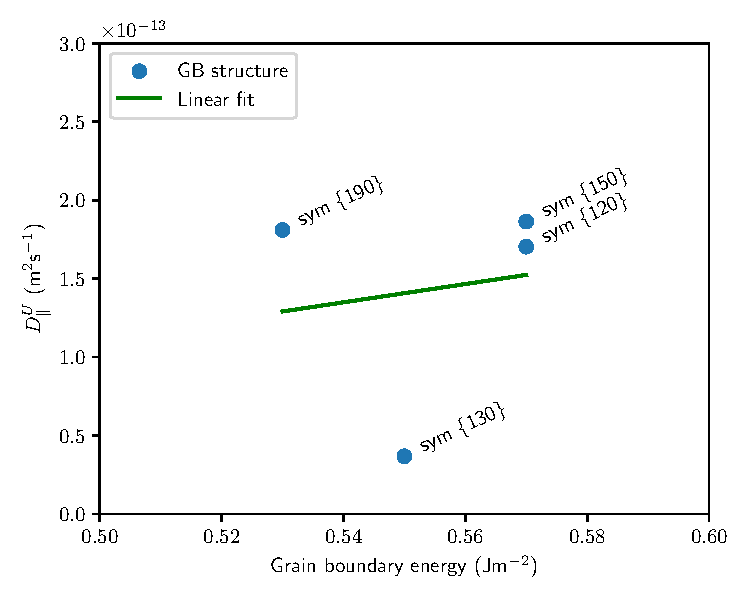
\includegraphics[width=\textwidth]{DvsGBE_600K.pdf}
    \end{subfigure}
    \begin{subfigure}{0.49\textwidth}
        \centering
        \caption{}
        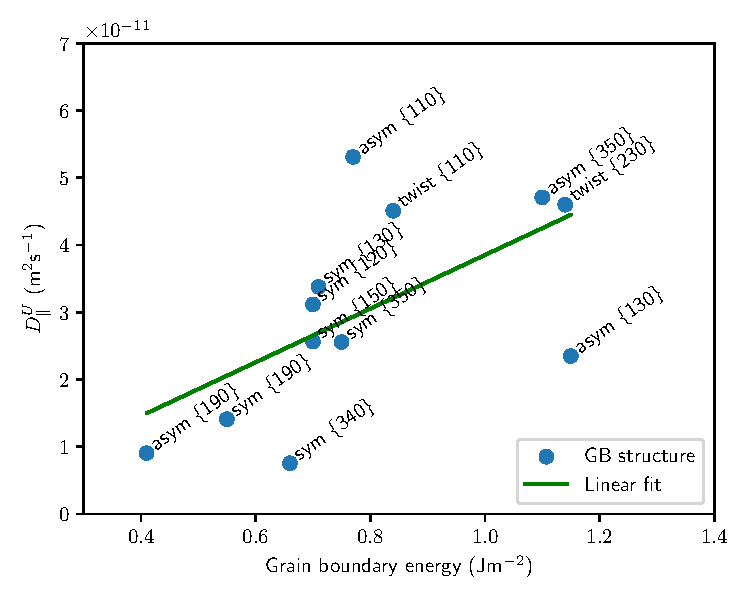
\includegraphics[width=\textwidth]{DvsGBE_1200K.pdf}
    \end{subfigure}
\caption{\DIFaddFL{Diffusion coefficient of U parallel to the tilt axis against grain boundary energy for various grain boundary structures at (a) 600 K and (b) 1200 K. The green lines are linear fits. $R^2$ scores are 0.02 and 0.36 for 600 K and 1200 K, respectively.}}
\label{fig:DvsGBE}
\end{figure}
\DIFaddend 

\end{appendices}


\FloatBarrier
\bibliographystyle{unsrt}
\bibliography{ref.bib}

\end{document}
